\documentclass{book}
\usepackage[a4paper,top=2.5cm,bottom=2.5cm,left=2.5cm,right=2.5cm]{geometry}
\usepackage{makeidx}
\usepackage{natbib}
\usepackage{graphicx}
\usepackage{multicol}
\usepackage{float}
\usepackage{listings}
\usepackage{color}
\usepackage{ifthen}
\usepackage[table]{xcolor}
\usepackage{textcomp}
\usepackage{alltt}
\usepackage{ifpdf}
\ifpdf
\usepackage[pdftex,
            pagebackref=true,
            colorlinks=true,
            linkcolor=blue,
            unicode
           ]{hyperref}
\else
\usepackage[ps2pdf,
            pagebackref=true,
            colorlinks=true,
            linkcolor=blue,
            unicode
           ]{hyperref}
\usepackage{pspicture}
\fi
\usepackage[utf8]{inputenc}
\usepackage{mathptmx}
\usepackage[scaled=.90]{helvet}
\usepackage{courier}
\usepackage{sectsty}
\usepackage{amssymb}
\usepackage[titles]{tocloft}
\usepackage{doxygen}
\lstset{language=C++,inputencoding=utf8,basicstyle=\footnotesize,breaklines=true,breakatwhitespace=true,tabsize=4,numbers=left }
\makeindex
\setcounter{tocdepth}{3}
\renewcommand{\footrulewidth}{0.4pt}
\renewcommand{\familydefault}{\sfdefault}
\hfuzz=15pt
\setlength{\emergencystretch}{15pt}
\hbadness=750
\tolerance=750
\begin{document}
\hypersetup{pageanchor=false,citecolor=blue}
\begin{titlepage}
\vspace*{7cm}
\begin{center}
{\Large short Path \\[1ex]\large 1.\-0 }\\
\vspace*{1cm}
{\large Generated by Doxygen 1.8.3.1}\\
\vspace*{0.5cm}
{\small Mon Aug 5 2013 00:16:25}\\
\end{center}
\end{titlepage}
\clearemptydoublepage
\pagenumbering{roman}
\tableofcontents
\clearemptydoublepage
\pagenumbering{arabic}
\hypersetup{pageanchor=true,citecolor=blue}
\chapter{The mainpage documentation}
\label{index}\hypertarget{index}{}Das Programm wurde von Julian Vollmer (s0525904) und Philip Stewart (s0525xxx) im Rahmen des Faches M31.\-2 Distributed Systems and Parallel Processing erstellt. Es Demonstriert die Suche des kürzesten Weges mit Hilfe des \hyperlink{class_dijkstra}{Dijkstra} Algorithmus. Zum einen Wurde die Berechnung mit Hilfe eines Threads durchgeführt, weiterhin es möglich die Berechnung auf mehrere Threads zu verteilen. Das Hauptmerkmal wurde auf den Speedup gelegt welche im direkten Vergleich bei Wahl des Menüpunktes {\ttfamily Zeige Vergleichstest} ausgeführt wird. 
\chapter{Class Index}
\section{Class List}
Here are the classes, structs, unions and interfaces with brief descriptions\-:\begin{DoxyCompactList}
\item\contentsline{section}{\hyperlink{class_dijkstra}{Dijkstra} }{\pageref{class_dijkstra}}{}
\item\contentsline{section}{\hyperlink{class_short_path}{Short\-Path} }{\pageref{class_short_path}}{}
\end{DoxyCompactList}

\chapter{File Index}
\section{File List}
Here is a list of all files with brief descriptions\-:\begin{DoxyCompactList}
\item\contentsline{section}{\hyperlink{main_8cpp}{main.\-cpp} }{\pageref{main_8cpp}}{}
\item\contentsline{section}{\hyperlink{main_8h}{main.\-h} }{\pageref{main_8h}}{}
\item\contentsline{section}{helper/\hyperlink{ausgabe_8cpp}{ausgabe.\-cpp} }{\pageref{ausgabe_8cpp}}{}
\item\contentsline{section}{helper/\hyperlink{ausgabe_8h}{ausgabe.\-h} }{\pageref{ausgabe_8h}}{}
\item\contentsline{section}{helper/\hyperlink{eingabe_8cpp}{eingabe.\-cpp} }{\pageref{eingabe_8cpp}}{}
\item\contentsline{section}{helper/\hyperlink{eingabe_8h}{eingabe.\-h} }{\pageref{eingabe_8h}}{}
\item\contentsline{section}{helper/\hyperlink{helpers_8cpp}{helpers.\-cpp} }{\pageref{helpers_8cpp}}{}
\item\contentsline{section}{helper/\hyperlink{helpers_8h}{helpers.\-h} }{\pageref{helpers_8h}}{}
\item\contentsline{section}{helper/\hyperlink{load__file_8cpp}{load\-\_\-file.\-cpp} }{\pageref{load__file_8cpp}}{}
\item\contentsline{section}{helper/\hyperlink{load__file_8h}{load\-\_\-file.\-h} }{\pageref{load__file_8h}}{}
\item\contentsline{section}{helper/\hyperlink{random_8cpp}{random.\-cpp} }{\pageref{random_8cpp}}{}
\item\contentsline{section}{helper/\hyperlink{random_8h}{random.\-h} }{\pageref{random_8h}}{}
\item\contentsline{section}{lib/\hyperlink{_dijkstra_8cpp}{Dijkstra.\-cpp} }{\pageref{_dijkstra_8cpp}}{}
\item\contentsline{section}{lib/\hyperlink{_dijkstra_8h}{Dijkstra.\-h} }{\pageref{_dijkstra_8h}}{}
\item\contentsline{section}{lib/\hyperlink{_path_element_8cpp}{Path\-Element.\-cpp} }{\pageref{_path_element_8cpp}}{}
\item\contentsline{section}{lib/\hyperlink{_path_element_8h}{Path\-Element.\-h} }{\pageref{_path_element_8h}}{}
\item\contentsline{section}{lib/\hyperlink{_path_vector_8cpp}{Path\-Vector.\-cpp} }{\pageref{_path_vector_8cpp}}{}
\item\contentsline{section}{lib/\hyperlink{_path_vector_8h}{Path\-Vector.\-h} }{\pageref{_path_vector_8h}}{}
\end{DoxyCompactList}

\chapter{Class Documentation}
\hypertarget{class_dijkstra}{\section{Dijkstra Class Reference}
\label{class_dijkstra}\index{Dijkstra@{Dijkstra}}
}


{\ttfamily \#include $<$Dijkstra.\-h$>$}

\subsection*{Public Member Functions}
\begin{DoxyCompactItemize}
\item 
void \hyperlink{class_dijkstra_a17070869ad646e4ac13a656b6f9adea4}{read} ()
\item 
void \hyperlink{class_dijkstra_a0f7f7f26abbe38dc975d1b73da1fd352}{initialize} ()
\item 
int \hyperlink{class_dijkstra_aa9df7dd7756870a4bb5ed14abfa93124}{get\-Closest\-Unmarked\-Node} ()
\item 
void \hyperlink{class_dijkstra_a110ea0c1486bf76fecec005f1eea56d0}{calculate\-Distance} ()
\item 
void \hyperlink{class_dijkstra_a267c5426563ba083712d16115bdf363b}{output} ()
\item 
void \hyperlink{class_dijkstra_a45305244759e1634249dc04438c3e207}{print\-Path} (int)
\item 
\hyperlink{class_dijkstra_ad7c7bb035ef96e4dbd652fe2bd11a2be}{Dijkstra} ()
\item 
string \hyperlink{class_dijkstra_a2673be1aaa7fbae0656239e66a855134}{get\-\_\-name} ()
\item 
int \hyperlink{class_dijkstra_af1d9287898152d9581fae471af19cf78}{get\-\_\-distance} ()
\item 
vector$<$ int $>$ \hyperlink{class_dijkstra_acd3b982f95ee25ed09184bb0da75f0b7}{get\-\_\-distances\-\_\-to\-\_\-other} ()
\item 
int \hyperlink{class_dijkstra_ad05e5384c101f91eded657061d1d9c30}{get\-\_\-predecessor} ()
\item 
bool \hyperlink{class_dijkstra_a1351e93ccbbfef5f0ce6dab8d4df2ac0}{get\-\_\-mark} ()
\item 
int \hyperlink{class_dijkstra_ab067a351a7c993cb900f64495e49aa4c}{get\-\_\-position} ()
\item 
int \hyperlink{class_dijkstra_af9bcc9baee081c08a7e192781788284f}{get\-\_\-distance\-\_\-from\-\_\-specific} (int position)
\item 
int \hyperlink{class_dijkstra_ac015491614e395f46f0c63171aef3be1}{get\-\_\-shortest\-\_\-distance} ()
\item 
void \hyperlink{class_dijkstra_a4e31f6a7349c13b57c9a41d4a6e5a7c7}{set\-\_\-name} (string name)
\item 
void \hyperlink{class_dijkstra_a0d5649f1baa5ce2d2c65b276141d6f40}{set\-\_\-predecessor} (int predecessor)
\item 
void \hyperlink{class_dijkstra_a75fcba38eab85c0fa15840a3d932156d}{set\-\_\-mark} (bool mark)
\item 
void \hyperlink{class_dijkstra_a8f857a9ebf93c48e0a6296e85b0d2524}{set\-\_\-position} (int position)
\item 
void \hyperlink{class_dijkstra_abed971366356f3ffcfbedaf1391c8d7e}{set\-\_\-distance\-\_\-vector} (vector$<$ int $>$ v)
\item 
void \hyperlink{class_dijkstra_a869289b1b15b665abf20bb04d6cc85c5}{set\-\_\-distance\-\_\-to\-\_\-specific} (int position, int value)
\item 
void \hyperlink{class_dijkstra_a85da246a755eebaf166f88af8e325107}{add\-\_\-distances\-\_\-to\-\_\-other} (int distance)
\item 
void \hyperlink{class_dijkstra_af69ad1ca6722e8c37eff60719506c330}{print\-\_\-distances} ()
\item 
void \hyperlink{class_dijkstra_aa6f64ceb0d55bf0c41af82534b5d0335}{init\-\_\-distances} ()
\end{DoxyCompactItemize}


\subsection{Detailed Description}


Definition at line 6 of file dk\-\_\-cpl.\-cpp.



\subsection{Constructor \& Destructor Documentation}
\hypertarget{class_dijkstra_ad7c7bb035ef96e4dbd652fe2bd11a2be}{\index{Dijkstra@{Dijkstra}!Dijkstra@{Dijkstra}}
\index{Dijkstra@{Dijkstra}!Dijkstra@{Dijkstra}}
\subsubsection[{Dijkstra}]{\setlength{\rightskip}{0pt plus 5cm}Dijkstra\-::\-Dijkstra (
\begin{DoxyParamCaption}
{}
\end{DoxyParamCaption}
)}}\label{class_dijkstra_ad7c7bb035ef96e4dbd652fe2bd11a2be}
Construktor 

Definition at line 8 of file Dijkstra.\-cpp.



Here is the call graph for this function\-:
\nopagebreak
\begin{figure}[H]
\begin{center}
\leavevmode
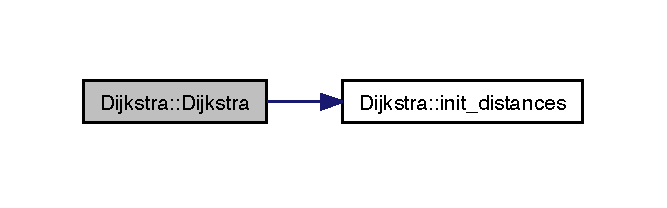
\includegraphics[width=320pt]{class_dijkstra_ad7c7bb035ef96e4dbd652fe2bd11a2be_cgraph}
\end{center}
\end{figure}




\subsection{Member Function Documentation}
\hypertarget{class_dijkstra_a85da246a755eebaf166f88af8e325107}{\index{Dijkstra@{Dijkstra}!add\-\_\-distances\-\_\-to\-\_\-other@{add\-\_\-distances\-\_\-to\-\_\-other}}
\index{add\-\_\-distances\-\_\-to\-\_\-other@{add\-\_\-distances\-\_\-to\-\_\-other}!Dijkstra@{Dijkstra}}
\subsubsection[{add\-\_\-distances\-\_\-to\-\_\-other}]{\setlength{\rightskip}{0pt plus 5cm}void Dijkstra\-::add\-\_\-distances\-\_\-to\-\_\-other (
\begin{DoxyParamCaption}
\item[{int}]{distance}
\end{DoxyParamCaption}
)}}\label{class_dijkstra_a85da246a755eebaf166f88af8e325107}
Adds a distance to the edge 
\begin{DoxyParams}{Parameters}
{\em distance} & distance to add \\
\hline
\end{DoxyParams}


Definition at line 143 of file Dijkstra.\-cpp.

\hypertarget{class_dijkstra_a110ea0c1486bf76fecec005f1eea56d0}{\index{Dijkstra@{Dijkstra}!calculate\-Distance@{calculate\-Distance}}
\index{calculate\-Distance@{calculate\-Distance}!Dijkstra@{Dijkstra}}
\subsubsection[{calculate\-Distance}]{\setlength{\rightskip}{0pt plus 5cm}void Dijkstra\-::calculate\-Distance (
\begin{DoxyParamCaption}
{}
\end{DoxyParamCaption}
)}}\label{class_dijkstra_a110ea0c1486bf76fecec005f1eea56d0}


Definition at line 107 of file dk\-\_\-cpl.\-cpp.



Here is the caller graph for this function\-:
\nopagebreak
\begin{figure}[H]
\begin{center}
\leavevmode
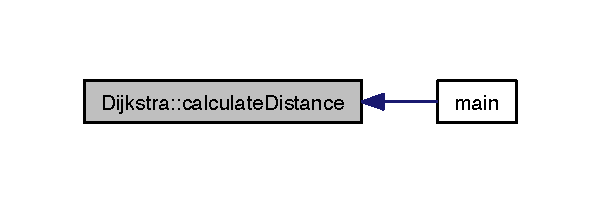
\includegraphics[width=288pt]{class_dijkstra_a110ea0c1486bf76fecec005f1eea56d0_icgraph}
\end{center}
\end{figure}


\hypertarget{class_dijkstra_af1d9287898152d9581fae471af19cf78}{\index{Dijkstra@{Dijkstra}!get\-\_\-distance@{get\-\_\-distance}}
\index{get\-\_\-distance@{get\-\_\-distance}!Dijkstra@{Dijkstra}}
\subsubsection[{get\-\_\-distance}]{\setlength{\rightskip}{0pt plus 5cm}int Dijkstra\-::get\-\_\-distance (
\begin{DoxyParamCaption}
{}
\end{DoxyParamCaption}
)}}\label{class_dijkstra_af1d9287898152d9581fae471af19cf78}
Returns the distance to the target edge \begin{DoxyReturn}{Returns}
Returns the distance to the target edge 
\end{DoxyReturn}


Definition at line 64 of file Dijkstra.\-cpp.

\hypertarget{class_dijkstra_af9bcc9baee081c08a7e192781788284f}{\index{Dijkstra@{Dijkstra}!get\-\_\-distance\-\_\-from\-\_\-specific@{get\-\_\-distance\-\_\-from\-\_\-specific}}
\index{get\-\_\-distance\-\_\-from\-\_\-specific@{get\-\_\-distance\-\_\-from\-\_\-specific}!Dijkstra@{Dijkstra}}
\subsubsection[{get\-\_\-distance\-\_\-from\-\_\-specific}]{\setlength{\rightskip}{0pt plus 5cm}int Dijkstra\-::get\-\_\-distance\-\_\-from\-\_\-specific (
\begin{DoxyParamCaption}
\item[{int}]{position}
\end{DoxyParamCaption}
)}}\label{class_dijkstra_af9bcc9baee081c08a7e192781788284f}
Returns the distance to a specific edge 
\begin{DoxyParams}{Parameters}
{\em position} & position of the edge \\
\hline
\end{DoxyParams}
\begin{DoxyReturn}{Returns}
distance 
\end{DoxyReturn}


Definition at line 36 of file Dijkstra.\-cpp.

\hypertarget{class_dijkstra_acd3b982f95ee25ed09184bb0da75f0b7}{\index{Dijkstra@{Dijkstra}!get\-\_\-distances\-\_\-to\-\_\-other@{get\-\_\-distances\-\_\-to\-\_\-other}}
\index{get\-\_\-distances\-\_\-to\-\_\-other@{get\-\_\-distances\-\_\-to\-\_\-other}!Dijkstra@{Dijkstra}}
\subsubsection[{get\-\_\-distances\-\_\-to\-\_\-other}]{\setlength{\rightskip}{0pt plus 5cm}vector$<$ int $>$ Dijkstra\-::get\-\_\-distances\-\_\-to\-\_\-other (
\begin{DoxyParamCaption}
{}
\end{DoxyParamCaption}
)}}\label{class_dijkstra_acd3b982f95ee25ed09184bb0da75f0b7}
Returns all distances to the other edges in a vector \begin{DoxyReturn}{Returns}

\end{DoxyReturn}


Definition at line 17 of file Dijkstra.\-cpp.

\hypertarget{class_dijkstra_a1351e93ccbbfef5f0ce6dab8d4df2ac0}{\index{Dijkstra@{Dijkstra}!get\-\_\-mark@{get\-\_\-mark}}
\index{get\-\_\-mark@{get\-\_\-mark}!Dijkstra@{Dijkstra}}
\subsubsection[{get\-\_\-mark}]{\setlength{\rightskip}{0pt plus 5cm}bool Dijkstra\-::get\-\_\-mark (
\begin{DoxyParamCaption}
{}
\end{DoxyParamCaption}
)}}\label{class_dijkstra_a1351e93ccbbfef5f0ce6dab8d4df2ac0}
Returns if a edge is visited or not \begin{DoxyReturn}{Returns}
Returns if a edge is visited or not 
\end{DoxyReturn}


Definition at line 80 of file Dijkstra.\-cpp.

\hypertarget{class_dijkstra_a2673be1aaa7fbae0656239e66a855134}{\index{Dijkstra@{Dijkstra}!get\-\_\-name@{get\-\_\-name}}
\index{get\-\_\-name@{get\-\_\-name}!Dijkstra@{Dijkstra}}
\subsubsection[{get\-\_\-name}]{\setlength{\rightskip}{0pt plus 5cm}string Dijkstra\-::get\-\_\-name (
\begin{DoxyParamCaption}
{}
\end{DoxyParamCaption}
)}}\label{class_dijkstra_a2673be1aaa7fbae0656239e66a855134}
Returns the name of the edge \begin{DoxyReturn}{Returns}
Returns the name of the edge 
\end{DoxyReturn}


Definition at line 56 of file Dijkstra.\-cpp.

\hypertarget{class_dijkstra_ab067a351a7c993cb900f64495e49aa4c}{\index{Dijkstra@{Dijkstra}!get\-\_\-position@{get\-\_\-position}}
\index{get\-\_\-position@{get\-\_\-position}!Dijkstra@{Dijkstra}}
\subsubsection[{get\-\_\-position}]{\setlength{\rightskip}{0pt plus 5cm}int Dijkstra\-::get\-\_\-position (
\begin{DoxyParamCaption}
{}
\end{DoxyParamCaption}
)}}\label{class_dijkstra_ab067a351a7c993cb900f64495e49aa4c}
Returns the position \begin{DoxyReturn}{Returns}
\mbox{[}description\mbox{]} 
\end{DoxyReturn}


Definition at line 88 of file Dijkstra.\-cpp.

\hypertarget{class_dijkstra_ad05e5384c101f91eded657061d1d9c30}{\index{Dijkstra@{Dijkstra}!get\-\_\-predecessor@{get\-\_\-predecessor}}
\index{get\-\_\-predecessor@{get\-\_\-predecessor}!Dijkstra@{Dijkstra}}
\subsubsection[{get\-\_\-predecessor}]{\setlength{\rightskip}{0pt plus 5cm}int Dijkstra\-::get\-\_\-predecessor (
\begin{DoxyParamCaption}
{}
\end{DoxyParamCaption}
)}}\label{class_dijkstra_ad05e5384c101f91eded657061d1d9c30}
Returns the predecessor \begin{DoxyReturn}{Returns}
Returns the predecessor 
\end{DoxyReturn}


Definition at line 72 of file Dijkstra.\-cpp.

\hypertarget{class_dijkstra_ac015491614e395f46f0c63171aef3be1}{\index{Dijkstra@{Dijkstra}!get\-\_\-shortest\-\_\-distance@{get\-\_\-shortest\-\_\-distance}}
\index{get\-\_\-shortest\-\_\-distance@{get\-\_\-shortest\-\_\-distance}!Dijkstra@{Dijkstra}}
\subsubsection[{get\-\_\-shortest\-\_\-distance}]{\setlength{\rightskip}{0pt plus 5cm}int Dijkstra\-::get\-\_\-shortest\-\_\-distance (
\begin{DoxyParamCaption}
{}
\end{DoxyParamCaption}
)}}\label{class_dijkstra_ac015491614e395f46f0c63171aef3be1}
Return the distance to the closest point \begin{DoxyReturn}{Returns}
distance 
\end{DoxyReturn}


Definition at line 95 of file Dijkstra.\-cpp.

\hypertarget{class_dijkstra_aa9df7dd7756870a4bb5ed14abfa93124}{\index{Dijkstra@{Dijkstra}!get\-Closest\-Unmarked\-Node@{get\-Closest\-Unmarked\-Node}}
\index{get\-Closest\-Unmarked\-Node@{get\-Closest\-Unmarked\-Node}!Dijkstra@{Dijkstra}}
\subsubsection[{get\-Closest\-Unmarked\-Node}]{\setlength{\rightskip}{0pt plus 5cm}int Dijkstra\-::get\-Closest\-Unmarked\-Node (
\begin{DoxyParamCaption}
{}
\end{DoxyParamCaption}
)}}\label{class_dijkstra_aa9df7dd7756870a4bb5ed14abfa93124}


Definition at line 94 of file dk\-\_\-cpl.\-cpp.

\hypertarget{class_dijkstra_aa6f64ceb0d55bf0c41af82534b5d0335}{\index{Dijkstra@{Dijkstra}!init\-\_\-distances@{init\-\_\-distances}}
\index{init\-\_\-distances@{init\-\_\-distances}!Dijkstra@{Dijkstra}}
\subsubsection[{init\-\_\-distances}]{\setlength{\rightskip}{0pt plus 5cm}void Dijkstra\-::init\-\_\-distances (
\begin{DoxyParamCaption}
{}
\end{DoxyParamCaption}
)}}\label{class_dijkstra_aa6f64ceb0d55bf0c41af82534b5d0335}
All distance has to be I\-N\-T\-\_\-\-M\-A\-X at the begining 

Definition at line 25 of file Dijkstra.\-cpp.



Here is the caller graph for this function\-:
\nopagebreak
\begin{figure}[H]
\begin{center}
\leavevmode
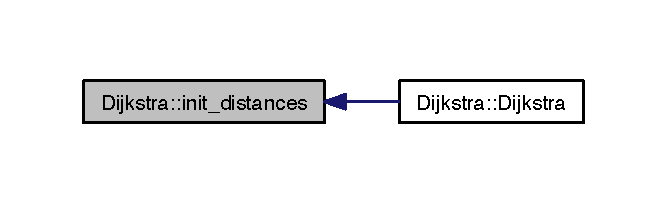
\includegraphics[width=320pt]{class_dijkstra_aa6f64ceb0d55bf0c41af82534b5d0335_icgraph}
\end{center}
\end{figure}


\hypertarget{class_dijkstra_a0f7f7f26abbe38dc975d1b73da1fd352}{\index{Dijkstra@{Dijkstra}!initialize@{initialize}}
\index{initialize@{initialize}!Dijkstra@{Dijkstra}}
\subsubsection[{initialize}]{\setlength{\rightskip}{0pt plus 5cm}void Dijkstra\-::initialize (
\begin{DoxyParamCaption}
{}
\end{DoxyParamCaption}
)}}\label{class_dijkstra_a0f7f7f26abbe38dc975d1b73da1fd352}


Definition at line 84 of file dk\-\_\-cpl.\-cpp.

\hypertarget{class_dijkstra_a267c5426563ba083712d16115bdf363b}{\index{Dijkstra@{Dijkstra}!output@{output}}
\index{output@{output}!Dijkstra@{Dijkstra}}
\subsubsection[{output}]{\setlength{\rightskip}{0pt plus 5cm}void Dijkstra\-::output (
\begin{DoxyParamCaption}
{}
\end{DoxyParamCaption}
)}}\label{class_dijkstra_a267c5426563ba083712d16115bdf363b}


Definition at line 140 of file dk\-\_\-cpl.\-cpp.



Here is the caller graph for this function\-:
\nopagebreak
\begin{figure}[H]
\begin{center}
\leavevmode
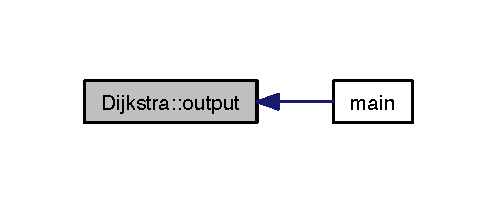
\includegraphics[width=238pt]{class_dijkstra_a267c5426563ba083712d16115bdf363b_icgraph}
\end{center}
\end{figure}


\hypertarget{class_dijkstra_af69ad1ca6722e8c37eff60719506c330}{\index{Dijkstra@{Dijkstra}!print\-\_\-distances@{print\-\_\-distances}}
\index{print\-\_\-distances@{print\-\_\-distances}!Dijkstra@{Dijkstra}}
\subsubsection[{print\-\_\-distances}]{\setlength{\rightskip}{0pt plus 5cm}void Dijkstra\-::print\-\_\-distances (
\begin{DoxyParamCaption}
{}
\end{DoxyParamCaption}
)}}\label{class_dijkstra_af69ad1ca6722e8c37eff60719506c330}
Prints the distance to the root edge 

Definition at line 159 of file Dijkstra.\-cpp.

\hypertarget{class_dijkstra_a45305244759e1634249dc04438c3e207}{\index{Dijkstra@{Dijkstra}!print\-Path@{print\-Path}}
\index{print\-Path@{print\-Path}!Dijkstra@{Dijkstra}}
\subsubsection[{print\-Path}]{\setlength{\rightskip}{0pt plus 5cm}void Dijkstra\-::print\-Path (
\begin{DoxyParamCaption}
\item[{int}]{node}
\end{DoxyParamCaption}
)}}\label{class_dijkstra_a45305244759e1634249dc04438c3e207}


Definition at line 128 of file dk\-\_\-cpl.\-cpp.

\hypertarget{class_dijkstra_a17070869ad646e4ac13a656b6f9adea4}{\index{Dijkstra@{Dijkstra}!read@{read}}
\index{read@{read}!Dijkstra@{Dijkstra}}
\subsubsection[{read}]{\setlength{\rightskip}{0pt plus 5cm}void Dijkstra\-::read (
\begin{DoxyParamCaption}
{}
\end{DoxyParamCaption}
)}}\label{class_dijkstra_a17070869ad646e4ac13a656b6f9adea4}


Definition at line 55 of file dk\-\_\-cpl.\-cpp.



Here is the caller graph for this function\-:
\nopagebreak
\begin{figure}[H]
\begin{center}
\leavevmode
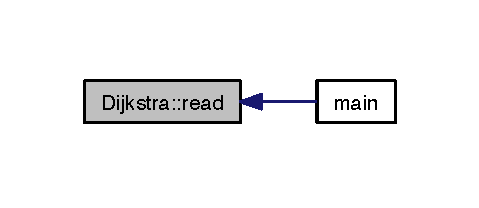
\includegraphics[width=230pt]{class_dijkstra_a17070869ad646e4ac13a656b6f9adea4_icgraph}
\end{center}
\end{figure}


\hypertarget{class_dijkstra_a869289b1b15b665abf20bb04d6cc85c5}{\index{Dijkstra@{Dijkstra}!set\-\_\-distance\-\_\-to\-\_\-specific@{set\-\_\-distance\-\_\-to\-\_\-specific}}
\index{set\-\_\-distance\-\_\-to\-\_\-specific@{set\-\_\-distance\-\_\-to\-\_\-specific}!Dijkstra@{Dijkstra}}
\subsubsection[{set\-\_\-distance\-\_\-to\-\_\-specific}]{\setlength{\rightskip}{0pt plus 5cm}void Dijkstra\-::set\-\_\-distance\-\_\-to\-\_\-specific (
\begin{DoxyParamCaption}
\item[{int}]{position, }
\item[{int}]{value}
\end{DoxyParamCaption}
)}}\label{class_dijkstra_a869289b1b15b665abf20bb04d6cc85c5}
Sets the distance to a specific edge 
\begin{DoxyParams}{Parameters}
{\em position} & target \\
\hline
{\em value} & distance \\
\hline
\end{DoxyParams}


Definition at line 48 of file Dijkstra.\-cpp.

\hypertarget{class_dijkstra_abed971366356f3ffcfbedaf1391c8d7e}{\index{Dijkstra@{Dijkstra}!set\-\_\-distance\-\_\-vector@{set\-\_\-distance\-\_\-vector}}
\index{set\-\_\-distance\-\_\-vector@{set\-\_\-distance\-\_\-vector}!Dijkstra@{Dijkstra}}
\subsubsection[{set\-\_\-distance\-\_\-vector}]{\setlength{\rightskip}{0pt plus 5cm}void Dijkstra\-::set\-\_\-distance\-\_\-vector (
\begin{DoxyParamCaption}
\item[{vector$<$ int $>$}]{v}
\end{DoxyParamCaption}
)}}\label{class_dijkstra_abed971366356f3ffcfbedaf1391c8d7e}
Sets a vector as distances 
\begin{DoxyParams}{Parameters}
{\em v} & vector with distances \\
\hline
\end{DoxyParams}


Definition at line 135 of file Dijkstra.\-cpp.



Here is the caller graph for this function\-:
\nopagebreak
\begin{figure}[H]
\begin{center}
\leavevmode
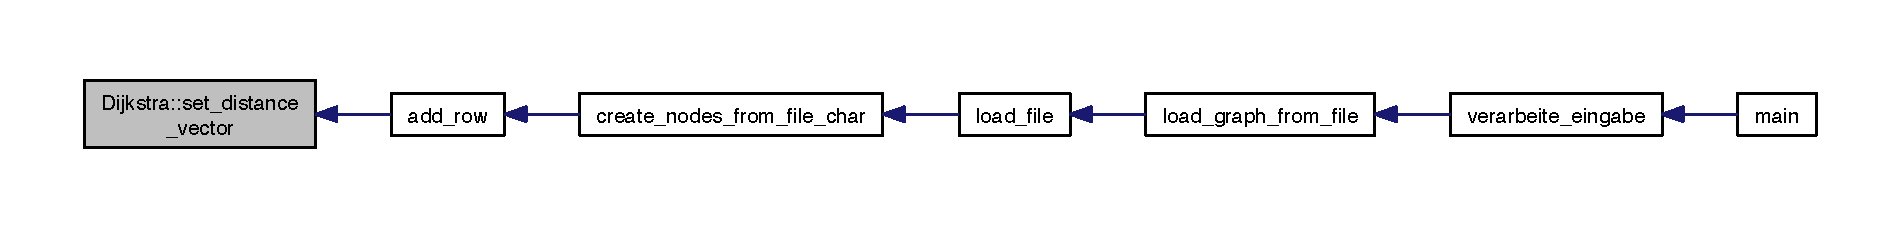
\includegraphics[width=350pt]{class_dijkstra_abed971366356f3ffcfbedaf1391c8d7e_icgraph}
\end{center}
\end{figure}


\hypertarget{class_dijkstra_a75fcba38eab85c0fa15840a3d932156d}{\index{Dijkstra@{Dijkstra}!set\-\_\-mark@{set\-\_\-mark}}
\index{set\-\_\-mark@{set\-\_\-mark}!Dijkstra@{Dijkstra}}
\subsubsection[{set\-\_\-mark}]{\setlength{\rightskip}{0pt plus 5cm}void Dijkstra\-::set\-\_\-mark (
\begin{DoxyParamCaption}
\item[{bool}]{mark}
\end{DoxyParamCaption}
)}}\label{class_dijkstra_a75fcba38eab85c0fa15840a3d932156d}
Return true if the egde was visited 
\begin{DoxyParams}{Parameters}
{\em mark} & true if visited \\
\hline
\end{DoxyParams}


Definition at line 127 of file Dijkstra.\-cpp.



Here is the caller graph for this function\-:
\nopagebreak
\begin{figure}[H]
\begin{center}
\leavevmode
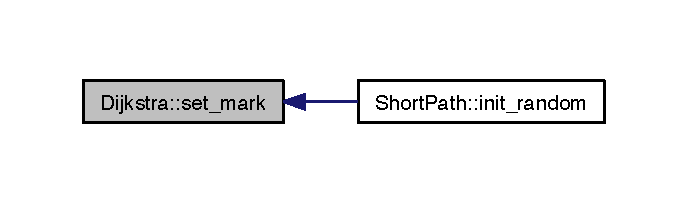
\includegraphics[width=330pt]{class_dijkstra_a75fcba38eab85c0fa15840a3d932156d_icgraph}
\end{center}
\end{figure}


\hypertarget{class_dijkstra_a4e31f6a7349c13b57c9a41d4a6e5a7c7}{\index{Dijkstra@{Dijkstra}!set\-\_\-name@{set\-\_\-name}}
\index{set\-\_\-name@{set\-\_\-name}!Dijkstra@{Dijkstra}}
\subsubsection[{set\-\_\-name}]{\setlength{\rightskip}{0pt plus 5cm}void Dijkstra\-::set\-\_\-name (
\begin{DoxyParamCaption}
\item[{string}]{name}
\end{DoxyParamCaption}
)}}\label{class_dijkstra_a4e31f6a7349c13b57c9a41d4a6e5a7c7}
Sets a name to the edge 
\begin{DoxyParams}{Parameters}
{\em name} & name to set \\
\hline
\end{DoxyParams}


Definition at line 111 of file Dijkstra.\-cpp.



Here is the caller graph for this function\-:
\nopagebreak
\begin{figure}[H]
\begin{center}
\leavevmode
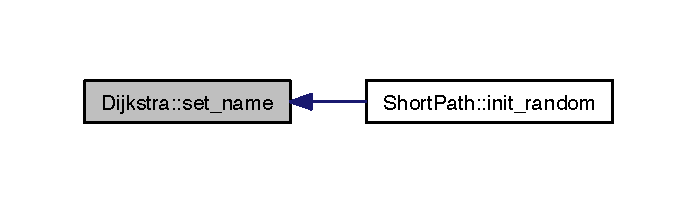
\includegraphics[width=334pt]{class_dijkstra_a4e31f6a7349c13b57c9a41d4a6e5a7c7_icgraph}
\end{center}
\end{figure}


\hypertarget{class_dijkstra_a8f857a9ebf93c48e0a6296e85b0d2524}{\index{Dijkstra@{Dijkstra}!set\-\_\-position@{set\-\_\-position}}
\index{set\-\_\-position@{set\-\_\-position}!Dijkstra@{Dijkstra}}
\subsubsection[{set\-\_\-position}]{\setlength{\rightskip}{0pt plus 5cm}void Dijkstra\-::set\-\_\-position (
\begin{DoxyParamCaption}
\item[{int}]{position}
\end{DoxyParamCaption}
)}}\label{class_dijkstra_a8f857a9ebf93c48e0a6296e85b0d2524}
Sets the position of a edge 
\begin{DoxyParams}{Parameters}
{\em position} & position as integer \\
\hline
\end{DoxyParams}


Definition at line 152 of file Dijkstra.\-cpp.



Here is the caller graph for this function\-:
\nopagebreak
\begin{figure}[H]
\begin{center}
\leavevmode
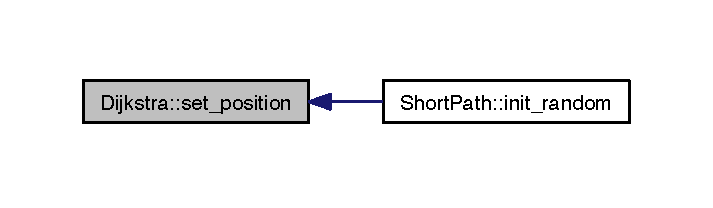
\includegraphics[width=342pt]{class_dijkstra_a8f857a9ebf93c48e0a6296e85b0d2524_icgraph}
\end{center}
\end{figure}


\hypertarget{class_dijkstra_a0d5649f1baa5ce2d2c65b276141d6f40}{\index{Dijkstra@{Dijkstra}!set\-\_\-predecessor@{set\-\_\-predecessor}}
\index{set\-\_\-predecessor@{set\-\_\-predecessor}!Dijkstra@{Dijkstra}}
\subsubsection[{set\-\_\-predecessor}]{\setlength{\rightskip}{0pt plus 5cm}void Dijkstra\-::set\-\_\-predecessor (
\begin{DoxyParamCaption}
\item[{int}]{predecessor}
\end{DoxyParamCaption}
)}}\label{class_dijkstra_a0d5649f1baa5ce2d2c65b276141d6f40}
Sets the predecessor 
\begin{DoxyParams}{Parameters}
{\em predecessor} & predecessor to set \\
\hline
\end{DoxyParams}


Definition at line 119 of file Dijkstra.\-cpp.



Here is the caller graph for this function\-:
\nopagebreak
\begin{figure}[H]
\begin{center}
\leavevmode
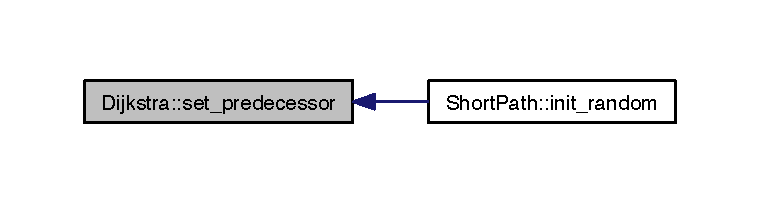
\includegraphics[width=350pt]{class_dijkstra_a0d5649f1baa5ce2d2c65b276141d6f40_icgraph}
\end{center}
\end{figure}




The documentation for this class was generated from the following files\-:\begin{DoxyCompactItemize}
\item 
\hyperlink{dk__cpl_8cpp}{dk\-\_\-cpl.\-cpp}\item 
lib/\hyperlink{_dijkstra_8h}{Dijkstra.\-h}\item 
lib/\hyperlink{_dijkstra_8cpp}{Dijkstra.\-cpp}\end{DoxyCompactItemize}

\hypertarget{class_short_path}{\section{Short\-Path Class Reference}
\label{class_short_path}\index{Short\-Path@{Short\-Path}}
}


{\ttfamily \#include $<$Short\-Path.\-h$>$}

\subsection*{Public Member Functions}
\begin{DoxyCompactItemize}
\item 
\hyperlink{class_short_path_aa1f54b3eb632252e0e4f34fed4110d54}{Short\-Path} ()
\item 
int \hyperlink{class_short_path_a04ad21508536061dc0f83aafa2fe25f3}{get\-\_\-num\-\_\-of\-\_\-vertices} ()
\item 
int \hyperlink{class_short_path_a82c56315bdb4245a028a060ab63dd866}{set\-\_\-source} (int src)
\item 
void \hyperlink{class_short_path_a113f044a61c1eacafb73df55e12f3803}{initialize} ()
\item 
int \hyperlink{class_short_path_ae218a65d8dd2620afc8c088679c5ab98}{get\-\_\-closest\-\_\-unmarked\-\_\-node} ()
\item 
void \hyperlink{class_short_path_af4ddb3c9a160c273bdc99b3fb43fd58d}{calculate\-\_\-distance} ()
\item 
void \hyperlink{class_short_path_a74f3fa59ffd3e061ef75a7962fbe3cfa}{calculate\-\_\-distance\-\_\-multiproc} ()
\item 
void \hyperlink{class_short_path_af65d23be9601ccf34becf9922c88c263}{add\-\_\-row} (\hyperlink{class_dijkstra}{Dijkstra} element)
\item 
void \hyperlink{class_short_path_aa4ede1b3713f60bef1f23193510199df}{output} ()
\item 
void \hyperlink{class_short_path_a24387db998bac1e88493dc4cf838a68b}{init\-\_\-random\-\_\-distances} ()
\item 
vector$<$ \hyperlink{class_dijkstra}{Dijkstra} $>$ \hyperlink{class_short_path_abf528c510136ea8014abfdd993949a02}{get\-\_\-elements} ()
\item 
void \hyperlink{class_short_path_a363cac67e1c10f524feab977073c35e9}{print\-Path} (int)
\item 
void \hyperlink{class_short_path_af3c6bd7d7b552ca6fa60b89a49db8566}{init\-\_\-random} ()
\item 
void \hyperlink{class_short_path_a1edee840fd8a1deec46d7c8ee4573bae}{init\-\_\-random} (int anz)
\item 
void \hyperlink{class_short_path_a388a3b66967f667a16b16f0f6fb044f3}{init\-\_\-source} ()
\item 
void \hyperlink{class_short_path_afa9098bdffcaaa0d77435dee10a2275f}{add\-\_\-random\-\_\-row} ()
\item 
void \hyperlink{class_short_path_a15edde62ae2c1a9f149815fb846c768e}{print} ()
\item 
void \hyperlink{class_short_path_a1c0cf18c306d022d72393979e37463c8}{clear} ()
\item 
int \hyperlink{class_short_path_a353d2a4cd4d25e57b4038f82ce3e1c79}{set\-\_\-number\-\_\-of\-\_\-threads} (int number)
\end{DoxyCompactItemize}


\subsection{Detailed Description}


Definition at line 23 of file Short\-Path.\-h.



\subsection{Constructor \& Destructor Documentation}
\hypertarget{class_short_path_aa1f54b3eb632252e0e4f34fed4110d54}{\index{Short\-Path@{Short\-Path}!Short\-Path@{Short\-Path}}
\index{Short\-Path@{Short\-Path}!ShortPath@{Short\-Path}}
\subsubsection[{Short\-Path}]{\setlength{\rightskip}{0pt plus 5cm}Short\-Path\-::\-Short\-Path (
\begin{DoxyParamCaption}
{}
\end{DoxyParamCaption}
)}}\label{class_short_path_aa1f54b3eb632252e0e4f34fed4110d54}
Constructor 

Definition at line 5 of file Short\-Path.\-cpp.



\subsection{Member Function Documentation}
\hypertarget{class_short_path_afa9098bdffcaaa0d77435dee10a2275f}{\index{Short\-Path@{Short\-Path}!add\-\_\-random\-\_\-row@{add\-\_\-random\-\_\-row}}
\index{add\-\_\-random\-\_\-row@{add\-\_\-random\-\_\-row}!ShortPath@{Short\-Path}}
\subsubsection[{add\-\_\-random\-\_\-row}]{\setlength{\rightskip}{0pt plus 5cm}void Short\-Path\-::add\-\_\-random\-\_\-row (
\begin{DoxyParamCaption}
{}
\end{DoxyParamCaption}
)}}\label{class_short_path_afa9098bdffcaaa0d77435dee10a2275f}
\hypertarget{class_short_path_af65d23be9601ccf34becf9922c88c263}{\index{Short\-Path@{Short\-Path}!add\-\_\-row@{add\-\_\-row}}
\index{add\-\_\-row@{add\-\_\-row}!ShortPath@{Short\-Path}}
\subsubsection[{add\-\_\-row}]{\setlength{\rightskip}{0pt plus 5cm}void Short\-Path\-::add\-\_\-row (
\begin{DoxyParamCaption}
\item[{{\bf Dijkstra}}]{element}
\end{DoxyParamCaption}
)}}\label{class_short_path_af65d23be9601ccf34becf9922c88c263}
Adds a row to the matrix 
\begin{DoxyParams}{Parameters}
{\em element} & \mbox{[}description\mbox{]} \\
\hline
\end{DoxyParams}


Definition at line 39 of file Short\-Path.\-cpp.



Here is the caller graph for this function\-:\nopagebreak
\begin{figure}[H]
\begin{center}
\leavevmode
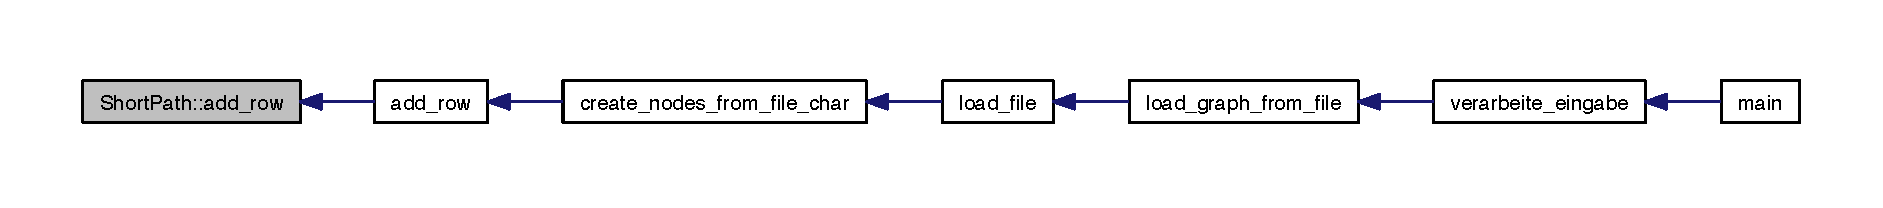
\includegraphics[width=350pt]{class_short_path_af65d23be9601ccf34becf9922c88c263_icgraph}
\end{center}
\end{figure}


\hypertarget{class_short_path_af4ddb3c9a160c273bdc99b3fb43fd58d}{\index{Short\-Path@{Short\-Path}!calculate\-\_\-distance@{calculate\-\_\-distance}}
\index{calculate\-\_\-distance@{calculate\-\_\-distance}!ShortPath@{Short\-Path}}
\subsubsection[{calculate\-\_\-distance}]{\setlength{\rightskip}{0pt plus 5cm}void Short\-Path\-::calculate\-\_\-distance (
\begin{DoxyParamCaption}
{}
\end{DoxyParamCaption}
)}}\label{class_short_path_af4ddb3c9a160c273bdc99b3fb43fd58d}
Function calculate\-\_\-distance calculates the minimum distances from the source node to other node. 

Definition at line 211 of file Short\-Path.\-cpp.



Here is the call graph for this function\-:\nopagebreak
\begin{figure}[H]
\begin{center}
\leavevmode
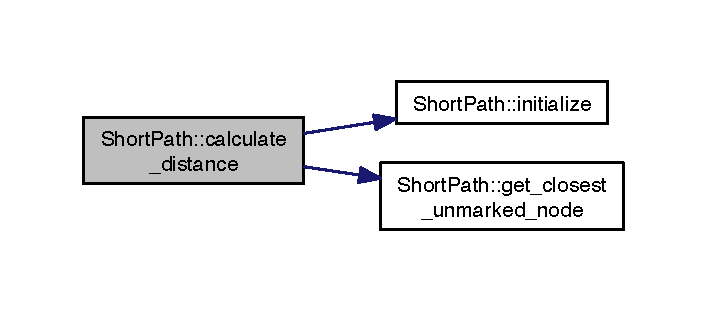
\includegraphics[width=340pt]{class_short_path_af4ddb3c9a160c273bdc99b3fb43fd58d_cgraph}
\end{center}
\end{figure}




Here is the caller graph for this function\-:
\nopagebreak
\begin{figure}[H]
\begin{center}
\leavevmode
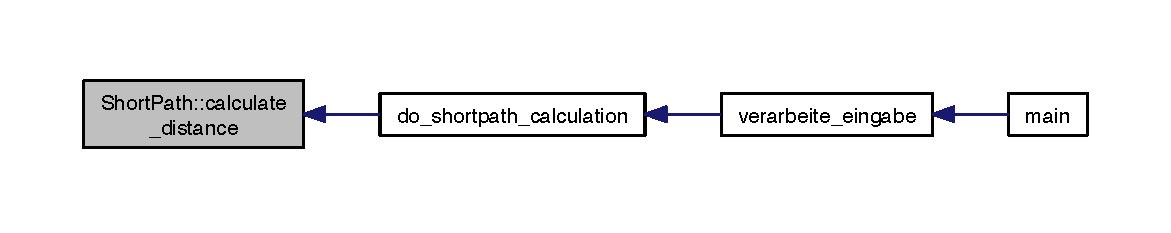
\includegraphics[width=350pt]{class_short_path_af4ddb3c9a160c273bdc99b3fb43fd58d_icgraph}
\end{center}
\end{figure}


\hypertarget{class_short_path_a74f3fa59ffd3e061ef75a7962fbe3cfa}{\index{Short\-Path@{Short\-Path}!calculate\-\_\-distance\-\_\-multiproc@{calculate\-\_\-distance\-\_\-multiproc}}
\index{calculate\-\_\-distance\-\_\-multiproc@{calculate\-\_\-distance\-\_\-multiproc}!ShortPath@{Short\-Path}}
\subsubsection[{calculate\-\_\-distance\-\_\-multiproc}]{\setlength{\rightskip}{0pt plus 5cm}void Short\-Path\-::calculate\-\_\-distance\-\_\-multiproc (
\begin{DoxyParamCaption}
{}
\end{DoxyParamCaption}
)}}\label{class_short_path_a74f3fa59ffd3e061ef75a7962fbe3cfa}
Function calculate\-\_\-distance calculates the minimum distances from the source node to other node. 

Definition at line 184 of file Short\-Path.\-cpp.



Here is the call graph for this function\-:\nopagebreak
\begin{figure}[H]
\begin{center}
\leavevmode
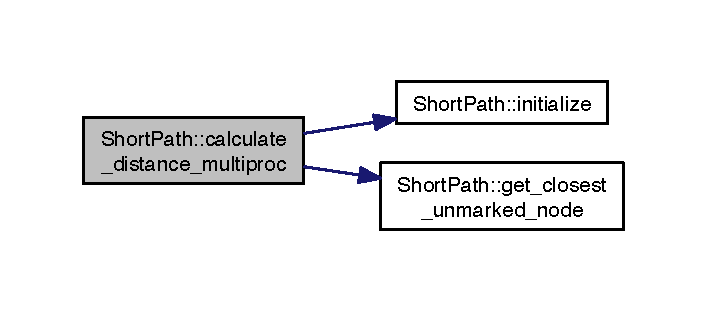
\includegraphics[width=340pt]{class_short_path_a74f3fa59ffd3e061ef75a7962fbe3cfa_cgraph}
\end{center}
\end{figure}




Here is the caller graph for this function\-:
\nopagebreak
\begin{figure}[H]
\begin{center}
\leavevmode
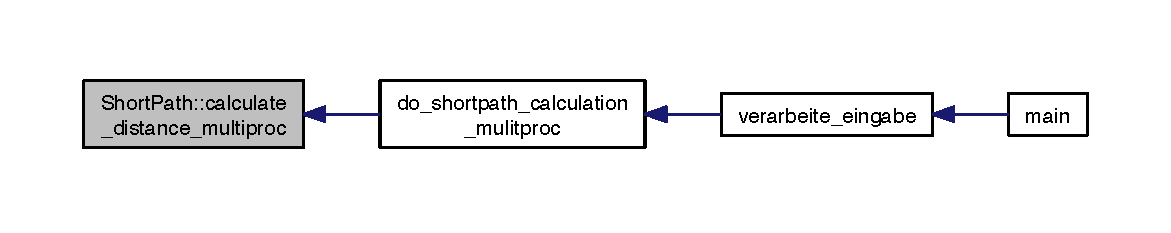
\includegraphics[width=350pt]{class_short_path_a74f3fa59ffd3e061ef75a7962fbe3cfa_icgraph}
\end{center}
\end{figure}


\hypertarget{class_short_path_a1c0cf18c306d022d72393979e37463c8}{\index{Short\-Path@{Short\-Path}!clear@{clear}}
\index{clear@{clear}!ShortPath@{Short\-Path}}
\subsubsection[{clear}]{\setlength{\rightskip}{0pt plus 5cm}void Short\-Path\-::clear (
\begin{DoxyParamCaption}
{}
\end{DoxyParamCaption}
)}}\label{class_short_path_a1c0cf18c306d022d72393979e37463c8}
Delete a elements 

Definition at line 19 of file Short\-Path.\-cpp.



Here is the caller graph for this function\-:\nopagebreak
\begin{figure}[H]
\begin{center}
\leavevmode
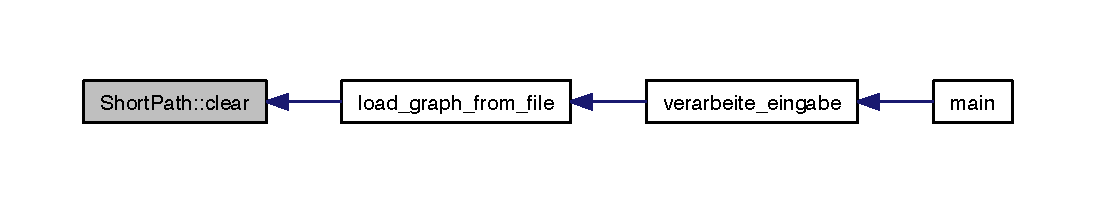
\includegraphics[width=350pt]{class_short_path_a1c0cf18c306d022d72393979e37463c8_icgraph}
\end{center}
\end{figure}


\hypertarget{class_short_path_ae218a65d8dd2620afc8c088679c5ab98}{\index{Short\-Path@{Short\-Path}!get\-\_\-closest\-\_\-unmarked\-\_\-node@{get\-\_\-closest\-\_\-unmarked\-\_\-node}}
\index{get\-\_\-closest\-\_\-unmarked\-\_\-node@{get\-\_\-closest\-\_\-unmarked\-\_\-node}!ShortPath@{Short\-Path}}
\subsubsection[{get\-\_\-closest\-\_\-unmarked\-\_\-node}]{\setlength{\rightskip}{0pt plus 5cm}int Short\-Path\-::get\-\_\-closest\-\_\-unmarked\-\_\-node (
\begin{DoxyParamCaption}
{}
\end{DoxyParamCaption}
)}}\label{class_short_path_ae218a65d8dd2620afc8c088679c5ab98}
Function get\-\_\-closed\-\_\-unmarked\-\_\-node returns the node which is nearest from the Predecessor marked node. If the node is already marked as visited, then it search for another node. \begin{DoxyReturn}{Returns}
closest\-\_\-unmarked\-\_\-node closest unmarked node 
\end{DoxyReturn}


Definition at line 168 of file Short\-Path.\-cpp.



Here is the caller graph for this function\-:
\nopagebreak
\begin{figure}[H]
\begin{center}
\leavevmode
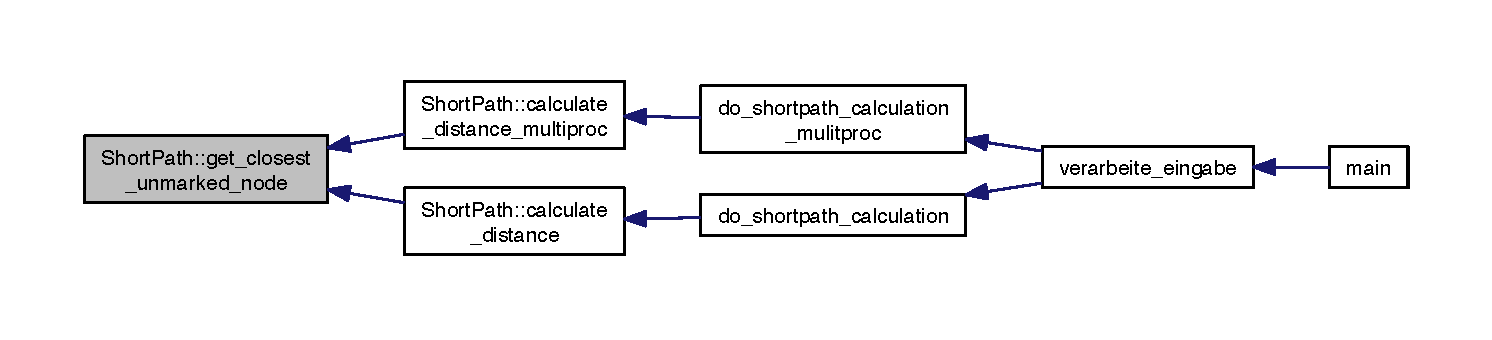
\includegraphics[width=350pt]{class_short_path_ae218a65d8dd2620afc8c088679c5ab98_icgraph}
\end{center}
\end{figure}


\hypertarget{class_short_path_abf528c510136ea8014abfdd993949a02}{\index{Short\-Path@{Short\-Path}!get\-\_\-elements@{get\-\_\-elements}}
\index{get\-\_\-elements@{get\-\_\-elements}!ShortPath@{Short\-Path}}
\subsubsection[{get\-\_\-elements}]{\setlength{\rightskip}{0pt plus 5cm}vector$<$ {\bf Dijkstra} $>$ Short\-Path\-::get\-\_\-elements (
\begin{DoxyParamCaption}
{}
\end{DoxyParamCaption}
)}}\label{class_short_path_abf528c510136ea8014abfdd993949a02}
\begin{DoxyReturn}{Returns}
Retuns all elements 
\end{DoxyReturn}


Definition at line 12 of file Short\-Path.\-cpp.



Here is the caller graph for this function\-:\nopagebreak
\begin{figure}[H]
\begin{center}
\leavevmode
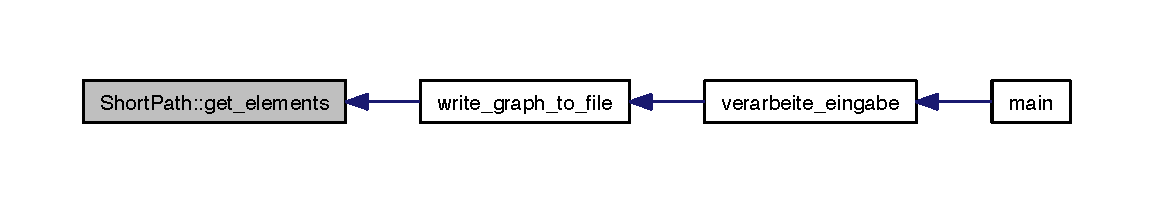
\includegraphics[width=350pt]{class_short_path_abf528c510136ea8014abfdd993949a02_icgraph}
\end{center}
\end{figure}


\hypertarget{class_short_path_a04ad21508536061dc0f83aafa2fe25f3}{\index{Short\-Path@{Short\-Path}!get\-\_\-num\-\_\-of\-\_\-vertices@{get\-\_\-num\-\_\-of\-\_\-vertices}}
\index{get\-\_\-num\-\_\-of\-\_\-vertices@{get\-\_\-num\-\_\-of\-\_\-vertices}!ShortPath@{Short\-Path}}
\subsubsection[{get\-\_\-num\-\_\-of\-\_\-vertices}]{\setlength{\rightskip}{0pt plus 5cm}int Short\-Path\-::get\-\_\-num\-\_\-of\-\_\-vertices (
\begin{DoxyParamCaption}
{}
\end{DoxyParamCaption}
)}}\label{class_short_path_a04ad21508536061dc0f83aafa2fe25f3}


Definition at line 23 of file Short\-Path.\-cpp.



Here is the caller graph for this function\-:
\nopagebreak
\begin{figure}[H]
\begin{center}
\leavevmode
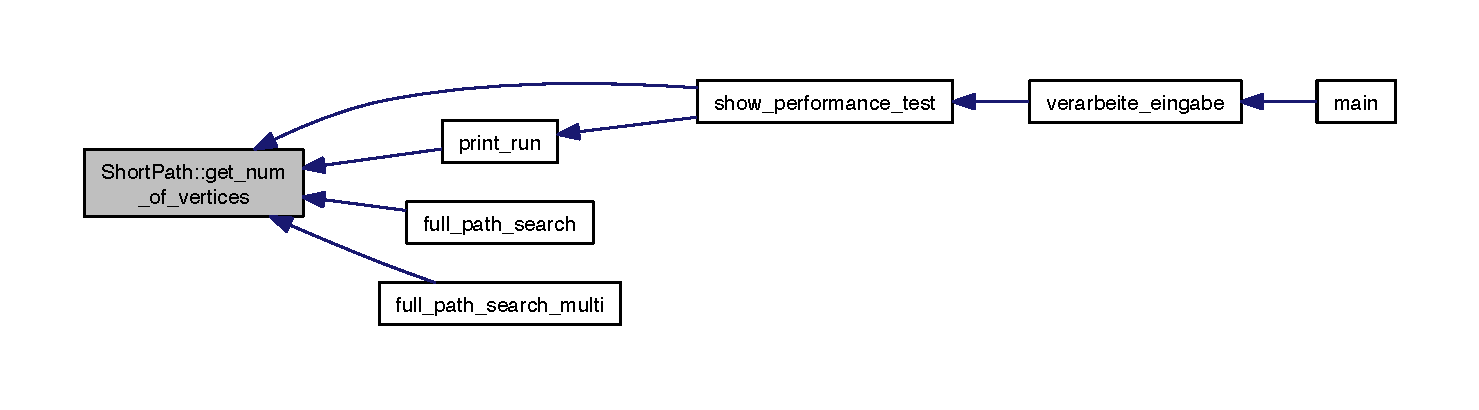
\includegraphics[width=350pt]{class_short_path_a04ad21508536061dc0f83aafa2fe25f3_icgraph}
\end{center}
\end{figure}


\hypertarget{class_short_path_af3c6bd7d7b552ca6fa60b89a49db8566}{\index{Short\-Path@{Short\-Path}!init\-\_\-random@{init\-\_\-random}}
\index{init\-\_\-random@{init\-\_\-random}!ShortPath@{Short\-Path}}
\subsubsection[{init\-\_\-random}]{\setlength{\rightskip}{0pt plus 5cm}void Short\-Path\-::init\-\_\-random (
\begin{DoxyParamCaption}
{}
\end{DoxyParamCaption}
)}}\label{class_short_path_af3c6bd7d7b552ca6fa60b89a49db8566}
initialize a Graph with a specific size 

Definition at line 132 of file Short\-Path.\-cpp.



Here is the call graph for this function\-:
\nopagebreak
\begin{figure}[H]
\begin{center}
\leavevmode
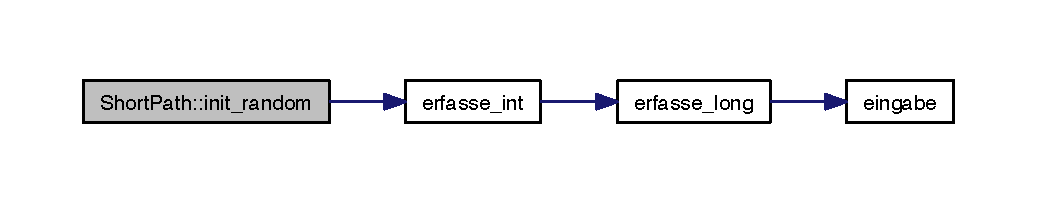
\includegraphics[width=350pt]{class_short_path_af3c6bd7d7b552ca6fa60b89a49db8566_cgraph}
\end{center}
\end{figure}




Here is the caller graph for this function\-:
\nopagebreak
\begin{figure}[H]
\begin{center}
\leavevmode
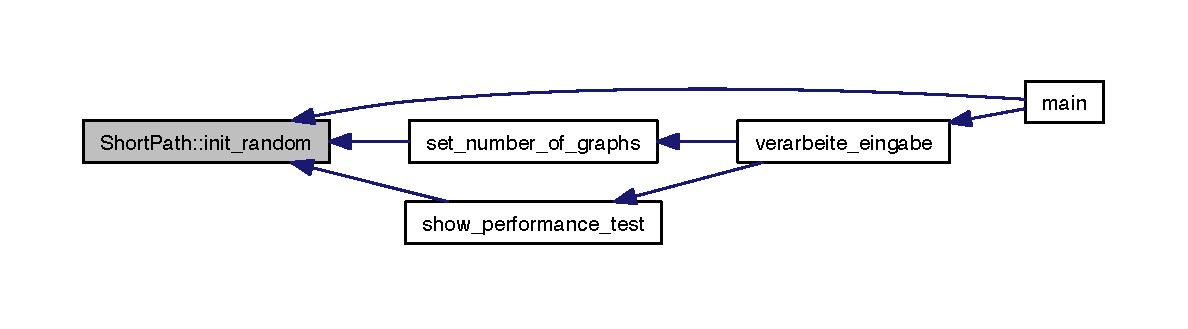
\includegraphics[width=350pt]{class_short_path_af3c6bd7d7b552ca6fa60b89a49db8566_icgraph}
\end{center}
\end{figure}


\hypertarget{class_short_path_a1edee840fd8a1deec46d7c8ee4573bae}{\index{Short\-Path@{Short\-Path}!init\-\_\-random@{init\-\_\-random}}
\index{init\-\_\-random@{init\-\_\-random}!ShortPath@{Short\-Path}}
\subsubsection[{init\-\_\-random}]{\setlength{\rightskip}{0pt plus 5cm}void Short\-Path\-::init\-\_\-random (
\begin{DoxyParamCaption}
\item[{int}]{anz}
\end{DoxyParamCaption}
)}}\label{class_short_path_a1edee840fd8a1deec46d7c8ee4573bae}
Initialize the random initialisation 
\begin{DoxyParams}{Parameters}
{\em anz} & \mbox{[}description\mbox{]} \\
\hline
\end{DoxyParams}


Definition at line 115 of file Short\-Path.\-cpp.



Here is the call graph for this function\-:\nopagebreak
\begin{figure}[H]
\begin{center}
\leavevmode
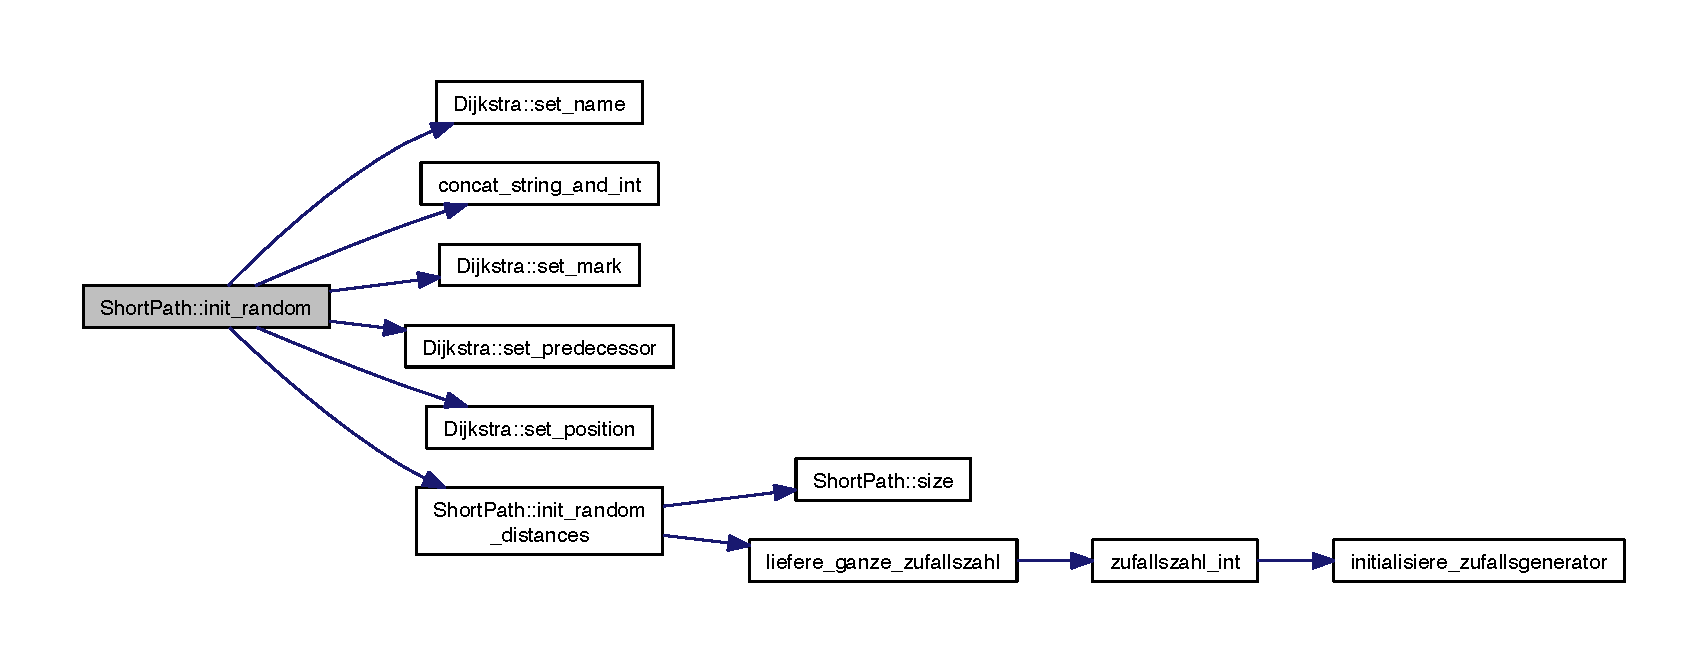
\includegraphics[width=350pt]{class_short_path_a1edee840fd8a1deec46d7c8ee4573bae_cgraph}
\end{center}
\end{figure}


\hypertarget{class_short_path_a24387db998bac1e88493dc4cf838a68b}{\index{Short\-Path@{Short\-Path}!init\-\_\-random\-\_\-distances@{init\-\_\-random\-\_\-distances}}
\index{init\-\_\-random\-\_\-distances@{init\-\_\-random\-\_\-distances}!ShortPath@{Short\-Path}}
\subsubsection[{init\-\_\-random\-\_\-distances}]{\setlength{\rightskip}{0pt plus 5cm}void Short\-Path\-::init\-\_\-random\-\_\-distances (
\begin{DoxyParamCaption}
{}
\end{DoxyParamCaption}
)}}\label{class_short_path_a24387db998bac1e88493dc4cf838a68b}
initialize the graph random 

Definition at line 45 of file Short\-Path.\-cpp.



Here is the call graph for this function\-:\nopagebreak
\begin{figure}[H]
\begin{center}
\leavevmode
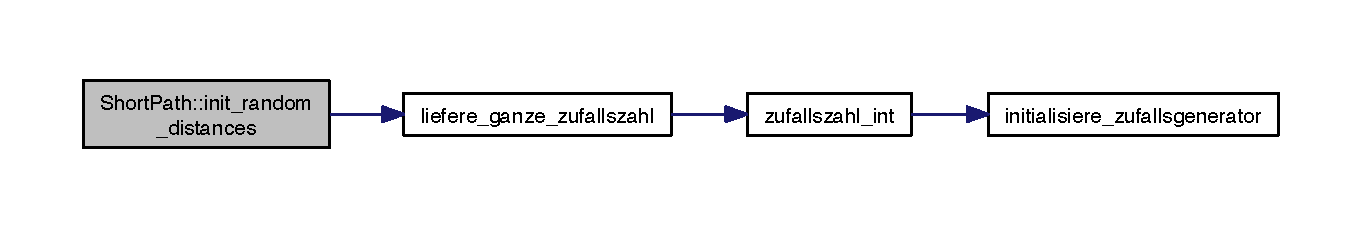
\includegraphics[width=350pt]{class_short_path_a24387db998bac1e88493dc4cf838a68b_cgraph}
\end{center}
\end{figure}




Here is the caller graph for this function\-:\nopagebreak
\begin{figure}[H]
\begin{center}
\leavevmode
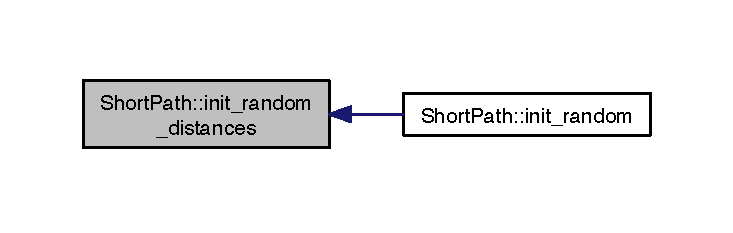
\includegraphics[width=350pt]{class_short_path_a24387db998bac1e88493dc4cf838a68b_icgraph}
\end{center}
\end{figure}


\hypertarget{class_short_path_a388a3b66967f667a16b16f0f6fb044f3}{\index{Short\-Path@{Short\-Path}!init\-\_\-source@{init\-\_\-source}}
\index{init\-\_\-source@{init\-\_\-source}!ShortPath@{Short\-Path}}
\subsubsection[{init\-\_\-source}]{\setlength{\rightskip}{0pt plus 5cm}void Short\-Path\-::init\-\_\-source (
\begin{DoxyParamCaption}
{}
\end{DoxyParamCaption}
)}}\label{class_short_path_a388a3b66967f667a16b16f0f6fb044f3}
\mbox{[}\hyperlink{class_short_path_a388a3b66967f667a16b16f0f6fb044f3}{Short\-Path\-::init\-\_\-source} description\mbox{]} 

Definition at line 140 of file Short\-Path.\-cpp.



Here is the call graph for this function\-:
\nopagebreak
\begin{figure}[H]
\begin{center}
\leavevmode
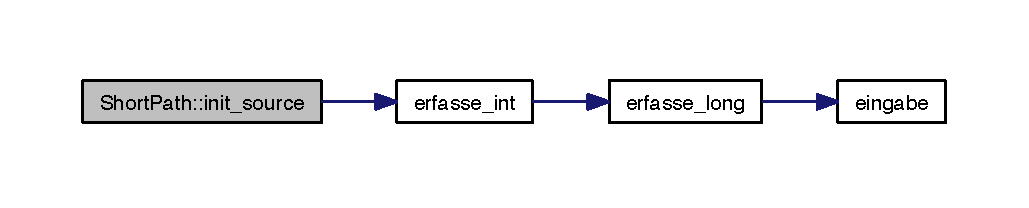
\includegraphics[width=350pt]{class_short_path_a388a3b66967f667a16b16f0f6fb044f3_cgraph}
\end{center}
\end{figure}


\hypertarget{class_short_path_a113f044a61c1eacafb73df55e12f3803}{\index{Short\-Path@{Short\-Path}!initialize@{initialize}}
\index{initialize@{initialize}!ShortPath@{Short\-Path}}
\subsubsection[{initialize}]{\setlength{\rightskip}{0pt plus 5cm}void Short\-Path\-::initialize (
\begin{DoxyParamCaption}
{}
\end{DoxyParamCaption}
)}}\label{class_short_path_a113f044a61c1eacafb73df55e12f3803}
Function initialize initializes all the data members at the begining of the execution. The distance between source to source is zero and all other distances between source and vertices are infinity. The mark is initialized to false and predecessor is initialized to -\/1 

Definition at line 151 of file Short\-Path.\-cpp.



Here is the caller graph for this function\-:
\nopagebreak
\begin{figure}[H]
\begin{center}
\leavevmode
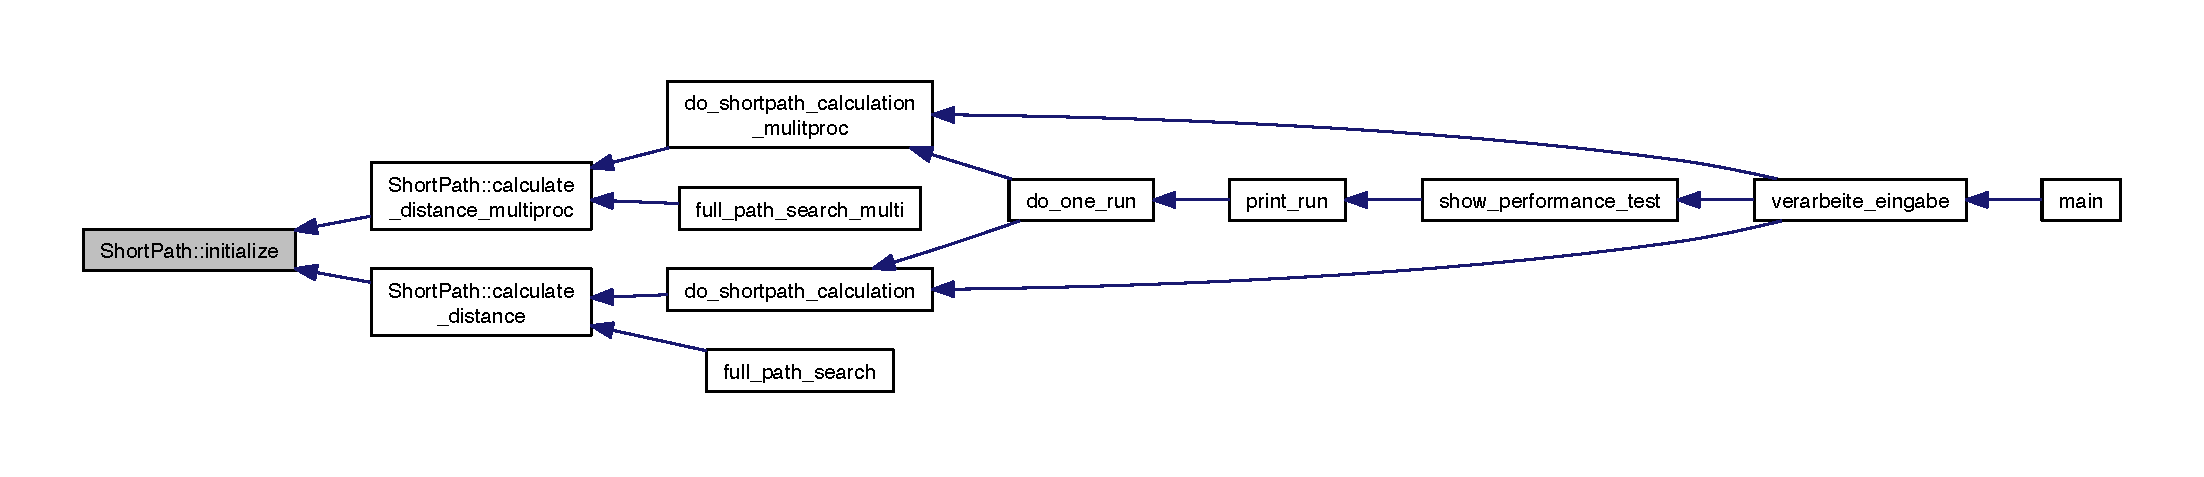
\includegraphics[width=350pt]{class_short_path_a113f044a61c1eacafb73df55e12f3803_icgraph}
\end{center}
\end{figure}


\hypertarget{class_short_path_aa4ede1b3713f60bef1f23193510199df}{\index{Short\-Path@{Short\-Path}!output@{output}}
\index{output@{output}!ShortPath@{Short\-Path}}
\subsubsection[{output}]{\setlength{\rightskip}{0pt plus 5cm}void Short\-Path\-::output (
\begin{DoxyParamCaption}
{}
\end{DoxyParamCaption}
)}}\label{class_short_path_aa4ede1b3713f60bef1f23193510199df}
print the output on the console 

Definition at line 253 of file Short\-Path.\-cpp.



Here is the call graph for this function\-:
\nopagebreak
\begin{figure}[H]
\begin{center}
\leavevmode
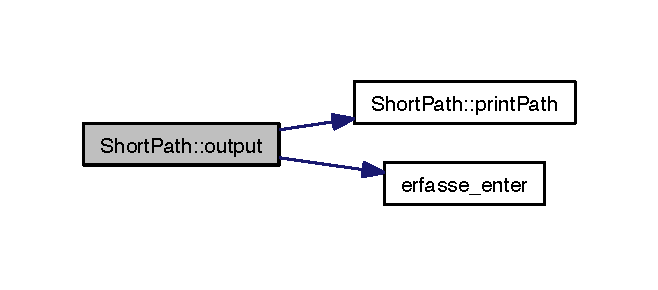
\includegraphics[width=316pt]{class_short_path_aa4ede1b3713f60bef1f23193510199df_cgraph}
\end{center}
\end{figure}




Here is the caller graph for this function\-:\nopagebreak
\begin{figure}[H]
\begin{center}
\leavevmode
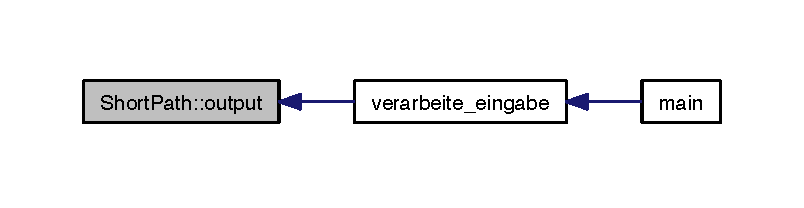
\includegraphics[width=350pt]{class_short_path_aa4ede1b3713f60bef1f23193510199df_icgraph}
\end{center}
\end{figure}


\hypertarget{class_short_path_a15edde62ae2c1a9f149815fb846c768e}{\index{Short\-Path@{Short\-Path}!print@{print}}
\index{print@{print}!ShortPath@{Short\-Path}}
\subsubsection[{print}]{\setlength{\rightskip}{0pt plus 5cm}void Short\-Path\-::print (
\begin{DoxyParamCaption}
{}
\end{DoxyParamCaption}
)}}\label{class_short_path_a15edde62ae2c1a9f149815fb846c768e}
prints the adjacency matrix. 

Definition at line 81 of file Short\-Path.\-cpp.



Here is the call graph for this function\-:
\nopagebreak
\begin{figure}[H]
\begin{center}
\leavevmode
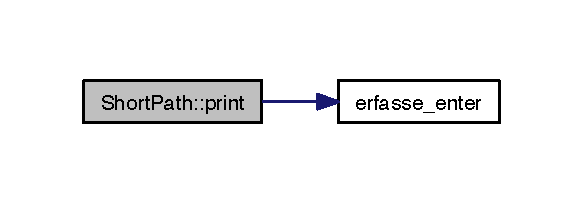
\includegraphics[width=280pt]{class_short_path_a15edde62ae2c1a9f149815fb846c768e_cgraph}
\end{center}
\end{figure}




Here is the caller graph for this function\-:\nopagebreak
\begin{figure}[H]
\begin{center}
\leavevmode
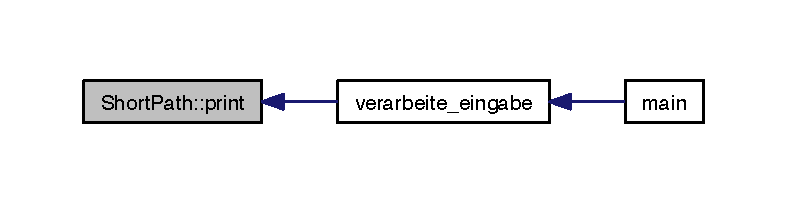
\includegraphics[width=350pt]{class_short_path_a15edde62ae2c1a9f149815fb846c768e_icgraph}
\end{center}
\end{figure}


\hypertarget{class_short_path_a363cac67e1c10f524feab977073c35e9}{\index{Short\-Path@{Short\-Path}!print\-Path@{print\-Path}}
\index{print\-Path@{print\-Path}!ShortPath@{Short\-Path}}
\subsubsection[{print\-Path}]{\setlength{\rightskip}{0pt plus 5cm}void Short\-Path\-::print\-Path (
\begin{DoxyParamCaption}
\item[{int}]{node}
\end{DoxyParamCaption}
)}}\label{class_short_path_a363cac67e1c10f524feab977073c35e9}
Prints the path to the node 
\begin{DoxyParams}{Parameters}
{\em node} & Node or target \\
\hline
\end{DoxyParams}


Definition at line 238 of file Short\-Path.\-cpp.



Here is the caller graph for this function\-:\nopagebreak
\begin{figure}[H]
\begin{center}
\leavevmode
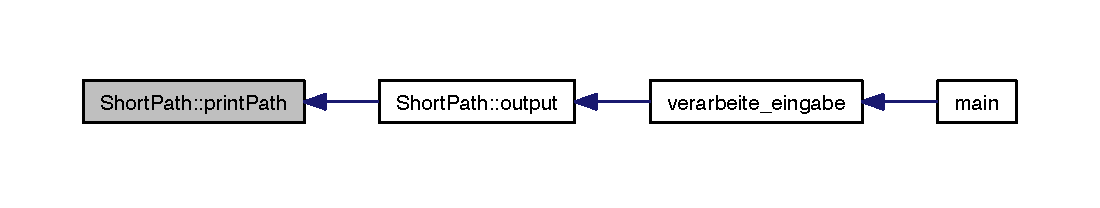
\includegraphics[width=350pt]{class_short_path_a363cac67e1c10f524feab977073c35e9_icgraph}
\end{center}
\end{figure}


\hypertarget{class_short_path_a353d2a4cd4d25e57b4038f82ce3e1c79}{\index{Short\-Path@{Short\-Path}!set\-\_\-number\-\_\-of\-\_\-threads@{set\-\_\-number\-\_\-of\-\_\-threads}}
\index{set\-\_\-number\-\_\-of\-\_\-threads@{set\-\_\-number\-\_\-of\-\_\-threads}!ShortPath@{Short\-Path}}
\subsubsection[{set\-\_\-number\-\_\-of\-\_\-threads}]{\setlength{\rightskip}{0pt plus 5cm}int Short\-Path\-::set\-\_\-number\-\_\-of\-\_\-threads (
\begin{DoxyParamCaption}
\item[{int}]{number}
\end{DoxyParamCaption}
)}}\label{class_short_path_a353d2a4cd4d25e57b4038f82ce3e1c79}


Definition at line 31 of file Short\-Path.\-cpp.



Here is the caller graph for this function\-:
\nopagebreak
\begin{figure}[H]
\begin{center}
\leavevmode
\includegraphics[width=350pt]{class_short_path_a353d2a4cd4d25e57b4038f82ce3e1c79_icgraph}
\end{center}
\end{figure}


\hypertarget{class_short_path_a82c56315bdb4245a028a060ab63dd866}{\index{Short\-Path@{Short\-Path}!set\-\_\-source@{set\-\_\-source}}
\index{set\-\_\-source@{set\-\_\-source}!ShortPath@{Short\-Path}}
\subsubsection[{set\-\_\-source}]{\setlength{\rightskip}{0pt plus 5cm}int Short\-Path\-::set\-\_\-source (
\begin{DoxyParamCaption}
\item[{int}]{src}
\end{DoxyParamCaption}
)}}\label{class_short_path_a82c56315bdb4245a028a060ab63dd866}


Definition at line 27 of file Short\-Path.\-cpp.



Here is the caller graph for this function\-:
\nopagebreak
\begin{figure}[H]
\begin{center}
\leavevmode
\includegraphics[width=348pt]{class_short_path_a82c56315bdb4245a028a060ab63dd866_icgraph}
\end{center}
\end{figure}




The documentation for this class was generated from the following files\-:\begin{DoxyCompactItemize}
\item 
lib/\hyperlink{_short_path_8h}{Short\-Path.\-h}\item 
lib/\hyperlink{_short_path_8cpp}{Short\-Path.\-cpp}\end{DoxyCompactItemize}

\chapter{File Documentation}
\hypertarget{dk__cpl_8cpp}{\section{dk\-\_\-cpl.\-cpp File Reference}
\label{dk__cpl_8cpp}\index{dk\-\_\-cpl.\-cpp@{dk\-\_\-cpl.\-cpp}}
}
{\ttfamily \#include $<$iostream$>$}\\*
Include dependency graph for dk\-\_\-cpl.\-cpp\-:\nopagebreak
\begin{figure}[H]
\begin{center}
\leavevmode
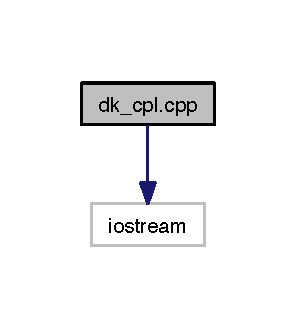
\includegraphics[width=142pt]{dk__cpl_8cpp__incl}
\end{center}
\end{figure}
\subsection*{Classes}
\begin{DoxyCompactItemize}
\item 
class \hyperlink{class_dijkstra}{Dijkstra}
\end{DoxyCompactItemize}
\subsection*{Macros}
\begin{DoxyCompactItemize}
\item 
\#define \hyperlink{dk__cpl_8cpp_a956e2723d559858d08644ac99146e910}{I\-N\-F\-I\-N\-I\-T\-Y}~999
\end{DoxyCompactItemize}
\subsection*{Functions}
\begin{DoxyCompactItemize}
\item 
int \hyperlink{dk__cpl_8cpp_ae66f6b31b5ad750f1fe042a706a4e3d4}{main} ()
\end{DoxyCompactItemize}


\subsection{Macro Definition Documentation}
\hypertarget{dk__cpl_8cpp_a956e2723d559858d08644ac99146e910}{\index{dk\-\_\-cpl.\-cpp@{dk\-\_\-cpl.\-cpp}!I\-N\-F\-I\-N\-I\-T\-Y@{I\-N\-F\-I\-N\-I\-T\-Y}}
\index{I\-N\-F\-I\-N\-I\-T\-Y@{I\-N\-F\-I\-N\-I\-T\-Y}!dk_cpl.cpp@{dk\-\_\-cpl.\-cpp}}
\subsubsection[{I\-N\-F\-I\-N\-I\-T\-Y}]{\setlength{\rightskip}{0pt plus 5cm}\#define I\-N\-F\-I\-N\-I\-T\-Y~999}}\label{dk__cpl_8cpp_a956e2723d559858d08644ac99146e910}


Definition at line 2 of file dk\-\_\-cpl.\-cpp.



\subsection{Function Documentation}
\hypertarget{dk__cpl_8cpp_ae66f6b31b5ad750f1fe042a706a4e3d4}{\index{dk\-\_\-cpl.\-cpp@{dk\-\_\-cpl.\-cpp}!main@{main}}
\index{main@{main}!dk_cpl.cpp@{dk\-\_\-cpl.\-cpp}}
\subsubsection[{main}]{\setlength{\rightskip}{0pt plus 5cm}int main (
\begin{DoxyParamCaption}
{}
\end{DoxyParamCaption}
)}}\label{dk__cpl_8cpp_ae66f6b31b5ad750f1fe042a706a4e3d4}


Definition at line 151 of file dk\-\_\-cpl.\-cpp.



Here is the call graph for this function\-:\nopagebreak
\begin{figure}[H]
\begin{center}
\leavevmode
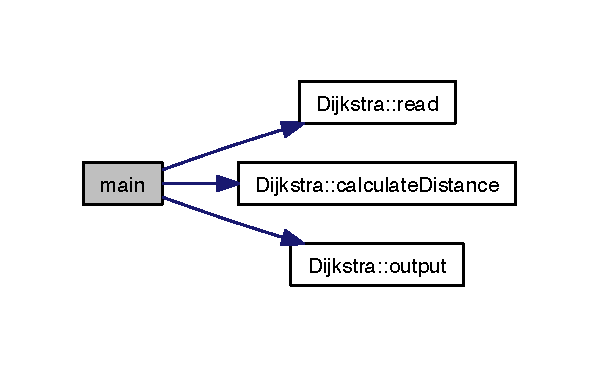
\includegraphics[width=288pt]{dk__cpl_8cpp_ae66f6b31b5ad750f1fe042a706a4e3d4_cgraph}
\end{center}
\end{figure}



\hypertarget{ausgabe_8cpp}{\section{helper/ausgabe.cpp File Reference}
\label{ausgabe_8cpp}\index{helper/ausgabe.\-cpp@{helper/ausgabe.\-cpp}}
}
{\ttfamily \#include \char`\"{}ausgabe.\-h\char`\"{}}\\*
Include dependency graph for ausgabe.\-cpp\-:
\nopagebreak
\begin{figure}[H]
\begin{center}
\leavevmode
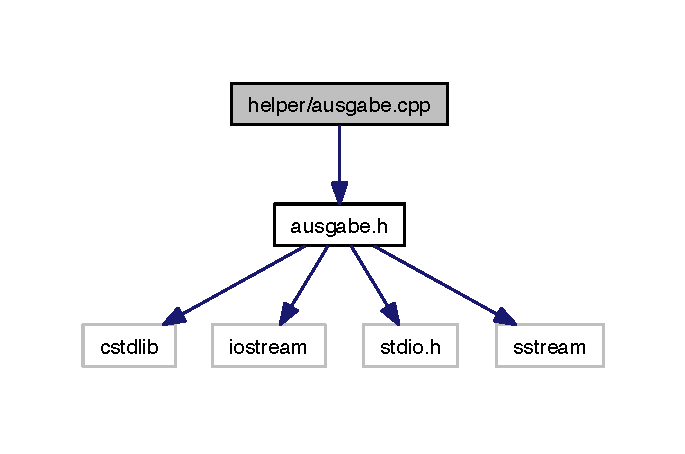
\includegraphics[width=329pt]{ausgabe_8cpp__incl}
\end{center}
\end{figure}
\subsection*{Functions}
\begin{DoxyCompactItemize}
\item 
void \hyperlink{ausgabe_8cpp_ae8c346aa92fc891022a940f2c5c75f95}{setze\-\_\-schalter} (ios\-\_\-base\-::fmtflags format)
\item 
void \hyperlink{ausgabe_8cpp_a3109f9f4c65293eb538b2697fda647c9}{schreibe\-\_\-zahl} (long zahl, ios\-\_\-base\-::fmtflags format\mbox{[}$\,$\mbox{]}, int anzahl\-\_\-formate)
\item 
void \hyperlink{ausgabe_8cpp_ad9369e6d8029bd00bba7b041ed0edfc8}{print\-\_\-number\-\_\-from\-\_\-matrix\-\_\-int} (int number)
\item 
void \hyperlink{ausgabe_8cpp_a4d7bb24e0d2df3eb7b8c30232f08e4cc}{print\-\_\-number\-\_\-from\-\_\-matrix\-\_\-double} (double number)
\item 
void \hyperlink{ausgabe_8cpp_af597975886c508e6ad4449837c23b61e}{schreibe\-\_\-zahl} (long zahl, ios\-\_\-base\-::fmtflags format)
\item 
void \hyperlink{ausgabe_8cpp_a9afeddc3a2e51a1d3c7e110fb16767cb}{schreibe\-\_\-zahl} (long zahl, streamsize feldbreite, ios\-\_\-base\-::fmtflags format\mbox{[}$\,$\mbox{]}, int anzahl\-\_\-formate)
\item 
void \hyperlink{ausgabe_8cpp_a0381140ca142dea69e5e466a45d8982c}{schreibe\-\_\-zahl} (long zahl, streamsize feldbreite, ios\-\_\-base\-::fmtflags format)
\item 
void \hyperlink{ausgabe_8cpp_ad67b1282696f63e5b34b1647d274077f}{schreibe\-\_\-zahl} (long zahl, streamsize feldbreite, char fuellzeichen, ios\-\_\-base\-::fmtflags format\mbox{[}$\,$\mbox{]}, int anzahl\-\_\-formate)
\item 
void \hyperlink{ausgabe_8cpp_a1665a46b00999bb8a0aca574ed0ed827}{schreibe\-\_\-zahl} (long zahl, streamsize feldbreite, char fuellzeichen, ios\-\_\-base\-::fmtflags format)
\item 
void \hyperlink{ausgabe_8cpp_ad428331d8837c1f886c98d996defa4c0}{schreibe\-\_\-zahl} (long double zahl, ios\-\_\-base\-::fmtflags format\mbox{[}$\,$\mbox{]}, int anzahl\-\_\-formate)
\item 
void \hyperlink{ausgabe_8cpp_af641fdccfc7fc8e61718fb3638e527e7}{schreibe\-\_\-zahl} (long double zahl, ios\-\_\-base\-::fmtflags format)
\item 
void \hyperlink{ausgabe_8cpp_a990c6f1274271b12da060a298a97412d}{schreibe\-\_\-zahl} (long double zahl, streamsize feldbreite, ios\-\_\-base\-::fmtflags format\mbox{[}$\,$\mbox{]}, int anzahl\-\_\-formate)
\item 
void \hyperlink{ausgabe_8cpp_a34b32ea150b542c42bd16e8d74832f43}{schreibe\-\_\-zahl} (long double zahl, streamsize feldbreite, ios\-\_\-base\-::fmtflags format)
\item 
void \hyperlink{ausgabe_8cpp_a7b6c3648ab9f0080c79ecb8aae689a0d}{schreibe\-\_\-zahl} (long double zahl, streamsize feldbreite, char fuellzeichen, ios\-\_\-base\-::fmtflags format\mbox{[}$\,$\mbox{]}, int anzahl\-\_\-formate)
\item 
void \hyperlink{ausgabe_8cpp_a7ee381ed414a7c21377514a823b3eb33}{schreibe\-\_\-zahl} (long double zahl, streamsize feldbreite, char fuellzeichen, ios\-\_\-base\-::fmtflags format\mbox{[}$\,$\mbox{]}, int anzahl\-\_\-formate, streamsize praezision)
\item 
void \hyperlink{ausgabe_8cpp_a9b4a59d38449fe87419fb125fc63ed93}{schreibe\-\_\-zahl} (double zahl, streamsize feldbreite, char fuellzeichen, ios\-\_\-base\-::fmtflags format\mbox{[}$\,$\mbox{]}, int anzahl\-\_\-formate)
\item 
void \hyperlink{ausgabe_8cpp_a5b12b6a0fe6cc5d43f63e6f72b1b2d45}{schreibe\-\_\-zahl} (int zahl, streamsize feldbreite, char fuellzeichen, ios\-\_\-base\-::fmtflags format\mbox{[}$\,$\mbox{]}, int anzahl\-\_\-formate)
\item 
void \hyperlink{ausgabe_8cpp_abf47c230eab9d30163dd908e4a1f65e7}{schreibe\-\_\-zahl} (long double zahl, streamsize feldbreite, char fuellzeichen, ios\-\_\-base\-::fmtflags format)
\item 
void \hyperlink{ausgabe_8cpp_aed6b39beca8a03fa3143258918f6253e}{schreibe\-\_\-zahl} (streamsize praezision, long double zahl, streamsize feldbreite, ios\-\_\-base\-::fmtflags format\mbox{[}$\,$\mbox{]}, int anzahl\-\_\-formate)
\item 
void \hyperlink{ausgabe_8cpp_ace96c319620ef24d874ccb41b42601f3}{zeige\-\_\-zahl\-\_\-von\-\_\-bis} (long double von, long double bis, long double abstand, streamsize praezision)
\item 
void \hyperlink{ausgabe_8cpp_a3737ce85b2d24f69b0960cebb26bea22}{zeige\-\_\-zahl} (double wert, streamsize praezision)
\item 
void \hyperlink{ausgabe_8cpp_abb46ef5c5d536396f1baa9c1a6ce1ccd}{spaltenvorschub} (streamsize feldbreite)
\item 
void \hyperlink{ausgabe_8cpp_a83c6a2f7b4a96e0c20b2119f3960022d}{loesche\-\_\-bildschirm} ()
\item 
void \hyperlink{ausgabe_8cpp_a5db6071f8d9d29f5e775bb27d50480a4}{loesche\-\_\-bildschirm\-\_\-mit\-\_\-header} ()
\item 
void \hyperlink{ausgabe_8cpp_a42662dc47ec6886db83f4fa886f87e32}{header} ()
\item 
void \hyperlink{ausgabe_8cpp_af8892c7dec59109baad426d539524dd6}{schreibe\-\_\-text} (string text, ios\-\_\-base\-::fmtflags format\mbox{[}$\,$\mbox{]}, int anzahl\-\_\-formate)
\item 
void \hyperlink{ausgabe_8cpp_a8124928a2d5ba8cb70d8368896ac6827}{schreibe\-\_\-text} (string text, streamsize feldbreite, char fuellzeichen, ios\-\_\-base\-::fmtflags format)
\item 
void \hyperlink{ausgabe_8cpp_a7b5a0354b89dacb17865e4735fea6a4f}{schreibe\-\_\-text} (string text, streamsize feldbreite)
\item 
void \hyperlink{ausgabe_8cpp_aeded53f62c8030087f76c69a5e974918}{schreibe\-\_\-text} (string text, streamsize feldbreite, char fuellzeichen)
\item 
void \hyperlink{ausgabe_8cpp_ab5931634ab2fd4e7863dd5be7d7f6b19}{schreibe\-\_\-text} (string text, streamsize feldbreite, ios\-\_\-base\-::fmtflags format\mbox{[}$\,$\mbox{]}, int anzahl\-\_\-formate)
\item 
void \hyperlink{ausgabe_8cpp_a2384f3389f4ad78d1c0f96058bef3024}{schreibe\-\_\-text} (string text, streamsize feldbreite, char fuellzeichen, ios\-\_\-base\-::fmtflags format\mbox{[}$\,$\mbox{]}, int anzahl\-\_\-formate)
\item 
void \hyperlink{ausgabe_8cpp_aa3b21853f890838c88d047d6c2786917}{wait} ()
\end{DoxyCompactItemize}


\subsection{Function Documentation}
\hypertarget{ausgabe_8cpp_a42662dc47ec6886db83f4fa886f87e32}{\index{ausgabe.\-cpp@{ausgabe.\-cpp}!header@{header}}
\index{header@{header}!ausgabe.cpp@{ausgabe.\-cpp}}
\subsubsection[{header}]{\setlength{\rightskip}{0pt plus 5cm}void header (
\begin{DoxyParamCaption}
{}
\end{DoxyParamCaption}
)}}\label{ausgabe_8cpp_a42662dc47ec6886db83f4fa886f87e32}
Schreibt einen Header fuer das Programm. 

Definition at line 309 of file ausgabe.\-cpp.



Here is the caller graph for this function\-:
\nopagebreak
\begin{figure}[H]
\begin{center}
\leavevmode
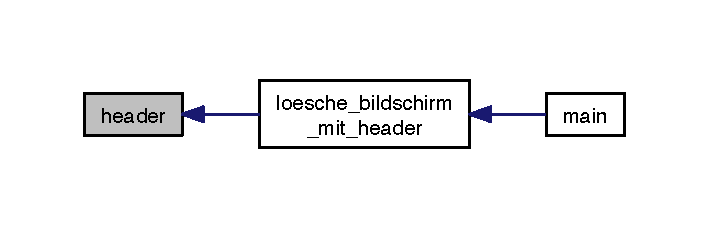
\includegraphics[width=340pt]{ausgabe_8cpp_a42662dc47ec6886db83f4fa886f87e32_icgraph}
\end{center}
\end{figure}


\hypertarget{ausgabe_8cpp_a83c6a2f7b4a96e0c20b2119f3960022d}{\index{ausgabe.\-cpp@{ausgabe.\-cpp}!loesche\-\_\-bildschirm@{loesche\-\_\-bildschirm}}
\index{loesche\-\_\-bildschirm@{loesche\-\_\-bildschirm}!ausgabe.cpp@{ausgabe.\-cpp}}
\subsubsection[{loesche\-\_\-bildschirm}]{\setlength{\rightskip}{0pt plus 5cm}void loesche\-\_\-bildschirm (
\begin{DoxyParamCaption}
{}
\end{DoxyParamCaption}
)}}\label{ausgabe_8cpp_a83c6a2f7b4a96e0c20b2119f3960022d}
Loescht den Bildschirminhalt der Konsole. 

Definition at line 296 of file ausgabe.\-cpp.



Here is the caller graph for this function\-:
\nopagebreak
\begin{figure}[H]
\begin{center}
\leavevmode
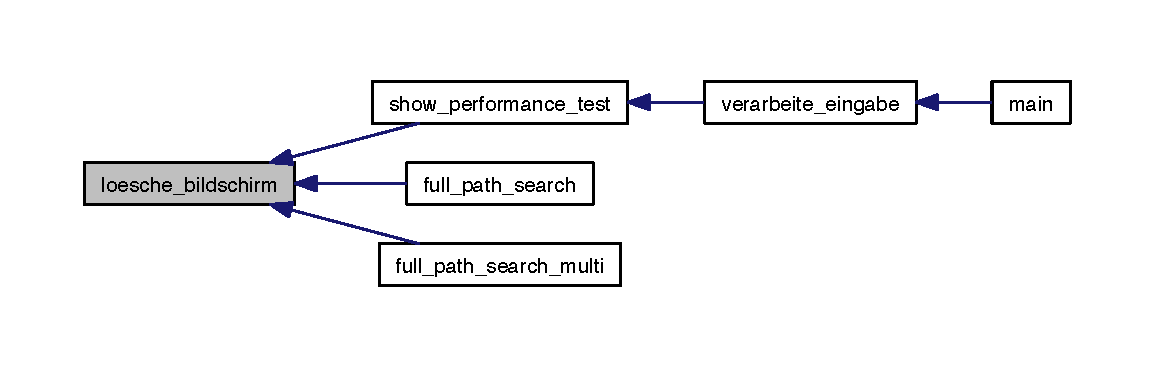
\includegraphics[width=350pt]{ausgabe_8cpp_a83c6a2f7b4a96e0c20b2119f3960022d_icgraph}
\end{center}
\end{figure}


\hypertarget{ausgabe_8cpp_a5db6071f8d9d29f5e775bb27d50480a4}{\index{ausgabe.\-cpp@{ausgabe.\-cpp}!loesche\-\_\-bildschirm\-\_\-mit\-\_\-header@{loesche\-\_\-bildschirm\-\_\-mit\-\_\-header}}
\index{loesche\-\_\-bildschirm\-\_\-mit\-\_\-header@{loesche\-\_\-bildschirm\-\_\-mit\-\_\-header}!ausgabe.cpp@{ausgabe.\-cpp}}
\subsubsection[{loesche\-\_\-bildschirm\-\_\-mit\-\_\-header}]{\setlength{\rightskip}{0pt plus 5cm}void loesche\-\_\-bildschirm\-\_\-mit\-\_\-header (
\begin{DoxyParamCaption}
{}
\end{DoxyParamCaption}
)}}\label{ausgabe_8cpp_a5db6071f8d9d29f5e775bb27d50480a4}
Loescht den Bildschirm der Konsole und schreibt den Header des Programmes. 

Definition at line 302 of file ausgabe.\-cpp.



Here is the call graph for this function\-:
\nopagebreak
\begin{figure}[H]
\begin{center}
\leavevmode
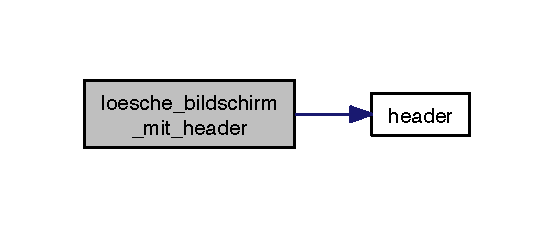
\includegraphics[width=266pt]{ausgabe_8cpp_a5db6071f8d9d29f5e775bb27d50480a4_cgraph}
\end{center}
\end{figure}




Here is the caller graph for this function\-:
\nopagebreak
\begin{figure}[H]
\begin{center}
\leavevmode
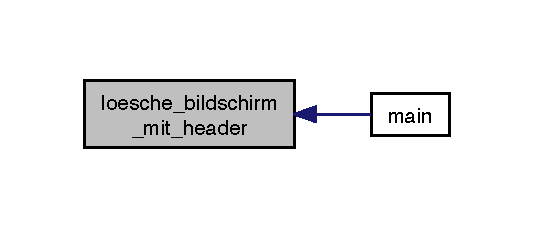
\includegraphics[width=256pt]{ausgabe_8cpp_a5db6071f8d9d29f5e775bb27d50480a4_icgraph}
\end{center}
\end{figure}


\hypertarget{ausgabe_8cpp_a4d7bb24e0d2df3eb7b8c30232f08e4cc}{\index{ausgabe.\-cpp@{ausgabe.\-cpp}!print\-\_\-number\-\_\-from\-\_\-matrix\-\_\-double@{print\-\_\-number\-\_\-from\-\_\-matrix\-\_\-double}}
\index{print\-\_\-number\-\_\-from\-\_\-matrix\-\_\-double@{print\-\_\-number\-\_\-from\-\_\-matrix\-\_\-double}!ausgabe.cpp@{ausgabe.\-cpp}}
\subsubsection[{print\-\_\-number\-\_\-from\-\_\-matrix\-\_\-double}]{\setlength{\rightskip}{0pt plus 5cm}void print\-\_\-number\-\_\-from\-\_\-matrix\-\_\-double (
\begin{DoxyParamCaption}
\item[{double}]{number}
\end{DoxyParamCaption}
)}}\label{ausgabe_8cpp_a4d7bb24e0d2df3eb7b8c30232f08e4cc}
Prints the number in the matrix. 
\begin{DoxyParams}{Parameters}
{\em number} & double value to print. \\
\hline
\end{DoxyParams}


Definition at line 50 of file ausgabe.\-cpp.



Here is the call graph for this function\-:
\nopagebreak
\begin{figure}[H]
\begin{center}
\leavevmode
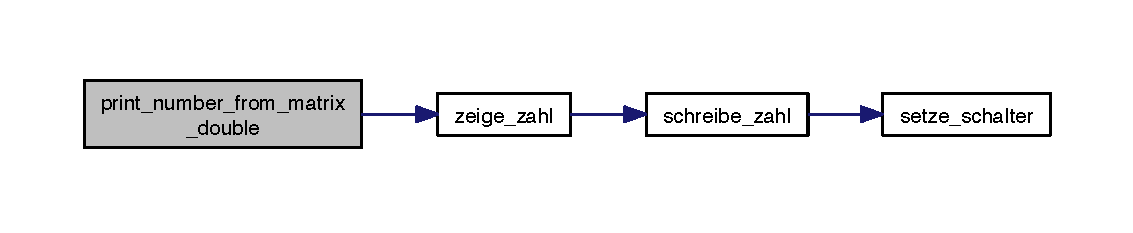
\includegraphics[width=350pt]{ausgabe_8cpp_a4d7bb24e0d2df3eb7b8c30232f08e4cc_cgraph}
\end{center}
\end{figure}




Here is the caller graph for this function\-:
\nopagebreak
\begin{figure}[H]
\begin{center}
\leavevmode
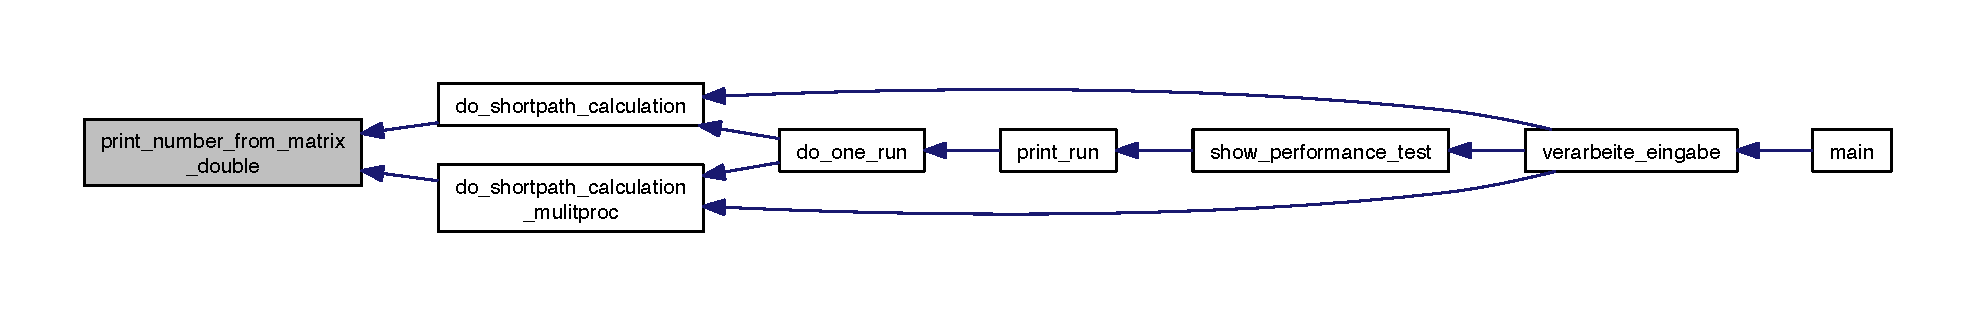
\includegraphics[width=350pt]{ausgabe_8cpp_a4d7bb24e0d2df3eb7b8c30232f08e4cc_icgraph}
\end{center}
\end{figure}


\hypertarget{ausgabe_8cpp_ad9369e6d8029bd00bba7b041ed0edfc8}{\index{ausgabe.\-cpp@{ausgabe.\-cpp}!print\-\_\-number\-\_\-from\-\_\-matrix\-\_\-int@{print\-\_\-number\-\_\-from\-\_\-matrix\-\_\-int}}
\index{print\-\_\-number\-\_\-from\-\_\-matrix\-\_\-int@{print\-\_\-number\-\_\-from\-\_\-matrix\-\_\-int}!ausgabe.cpp@{ausgabe.\-cpp}}
\subsubsection[{print\-\_\-number\-\_\-from\-\_\-matrix\-\_\-int}]{\setlength{\rightskip}{0pt plus 5cm}void print\-\_\-number\-\_\-from\-\_\-matrix\-\_\-int (
\begin{DoxyParamCaption}
\item[{int}]{number}
\end{DoxyParamCaption}
)}}\label{ausgabe_8cpp_ad9369e6d8029bd00bba7b041ed0edfc8}
Prints the number in the matrix. 
\begin{DoxyParams}{Parameters}
{\em number} & integer value to print. \\
\hline
\end{DoxyParams}


Definition at line 38 of file ausgabe.\-cpp.



Here is the call graph for this function\-:
\nopagebreak
\begin{figure}[H]
\begin{center}
\leavevmode
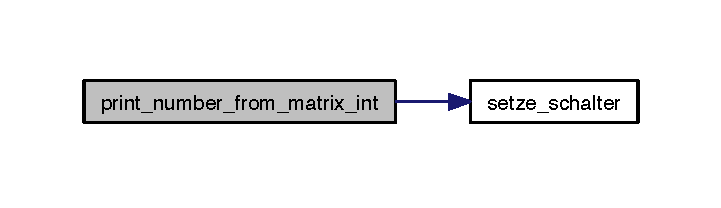
\includegraphics[width=346pt]{ausgabe_8cpp_ad9369e6d8029bd00bba7b041ed0edfc8_cgraph}
\end{center}
\end{figure}




Here is the caller graph for this function\-:
\nopagebreak
\begin{figure}[H]
\begin{center}
\leavevmode
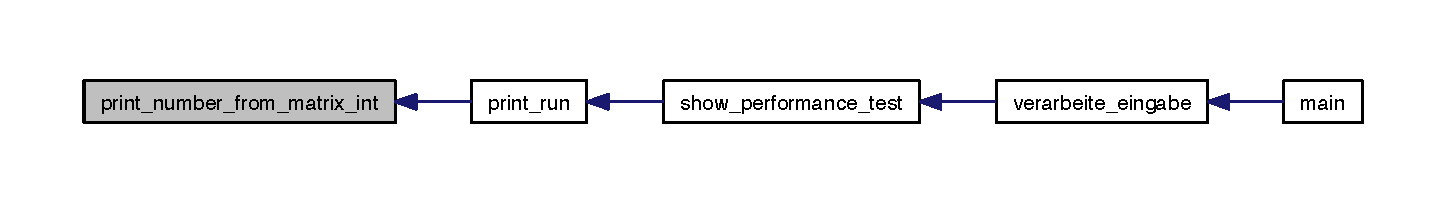
\includegraphics[width=350pt]{ausgabe_8cpp_ad9369e6d8029bd00bba7b041ed0edfc8_icgraph}
\end{center}
\end{figure}


\hypertarget{ausgabe_8cpp_af8892c7dec59109baad426d539524dd6}{\index{ausgabe.\-cpp@{ausgabe.\-cpp}!schreibe\-\_\-text@{schreibe\-\_\-text}}
\index{schreibe\-\_\-text@{schreibe\-\_\-text}!ausgabe.cpp@{ausgabe.\-cpp}}
\subsubsection[{schreibe\-\_\-text}]{\setlength{\rightskip}{0pt plus 5cm}void schreibe\-\_\-text (
\begin{DoxyParamCaption}
\item[{string}]{text, }
\item[{ios\-\_\-base\-::fmtflags}]{format\mbox{[}$\,$\mbox{]}, }
\item[{int}]{anzahl\-\_\-formate}
\end{DoxyParamCaption}
)}}\label{ausgabe_8cpp_af8892c7dec59109baad426d539524dd6}
Setzt verschiendene Schalter zu Steuerung und Formatierung der Ausgabe und schreibt einen Text auf den Bildschirm. 
\begin{DoxyParams}{Parameters}
{\em text} & Text der ausgegeben werden soll. \\
\hline
{\em format} & Formatierung die vorgenommen werden soll. \\
\hline
{\em anzahl\-\_\-formate} & Formatierung die vorgenommen werden soll. \\
\hline
\end{DoxyParams}


Definition at line 323 of file ausgabe.\-cpp.



Here is the call graph for this function\-:
\nopagebreak
\begin{figure}[H]
\begin{center}
\leavevmode
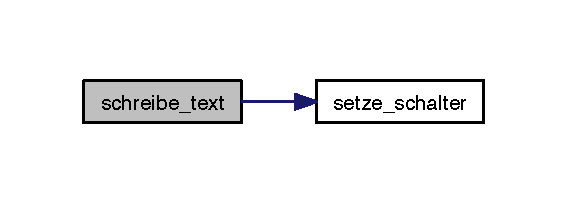
\includegraphics[width=272pt]{ausgabe_8cpp_af8892c7dec59109baad426d539524dd6_cgraph}
\end{center}
\end{figure}




Here is the caller graph for this function\-:
\nopagebreak
\begin{figure}[H]
\begin{center}
\leavevmode
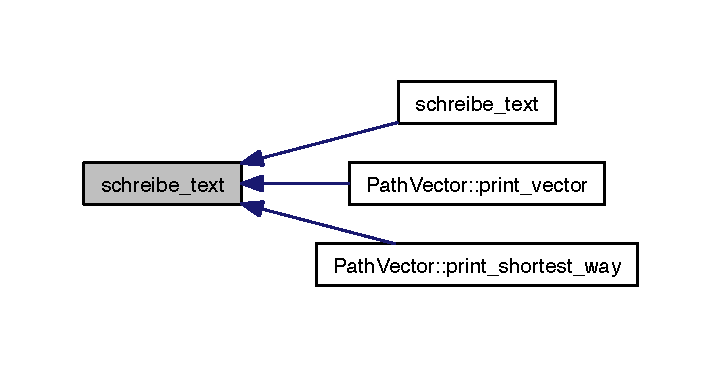
\includegraphics[width=268pt]{ausgabe_8cpp_af8892c7dec59109baad426d539524dd6_icgraph}
\end{center}
\end{figure}


\hypertarget{ausgabe_8cpp_a8124928a2d5ba8cb70d8368896ac6827}{\index{ausgabe.\-cpp@{ausgabe.\-cpp}!schreibe\-\_\-text@{schreibe\-\_\-text}}
\index{schreibe\-\_\-text@{schreibe\-\_\-text}!ausgabe.cpp@{ausgabe.\-cpp}}
\subsubsection[{schreibe\-\_\-text}]{\setlength{\rightskip}{0pt plus 5cm}void schreibe\-\_\-text (
\begin{DoxyParamCaption}
\item[{string}]{text, }
\item[{streamsize}]{feldbreite, }
\item[{char}]{fuellzeichen, }
\item[{ios\-\_\-base\-::fmtflags}]{format}
\end{DoxyParamCaption}
)}}\label{ausgabe_8cpp_a8124928a2d5ba8cb70d8368896ac6827}
Setzt verschiendene Schalter zu Steuerung und Formatierung der Ausgabe und schreibt einen Text auf den Bildschirm. 
\begin{DoxyParams}{Parameters}
{\em text} & Text der ausgegeben werden soll. \\
\hline
{\em feldbreite} & Feldbreite welche die Zahl haben soll. \\
\hline
{\em fuellzeichen} & Zeichen mit dem die restliche Feldbreite aufgefuellt werden soll. \\
\hline
{\em format} & Formatierung die vorgenommen werden soll. \\
\hline
\end{DoxyParams}


Definition at line 339 of file ausgabe.\-cpp.



Here is the call graph for this function\-:
\nopagebreak
\begin{figure}[H]
\begin{center}
\leavevmode
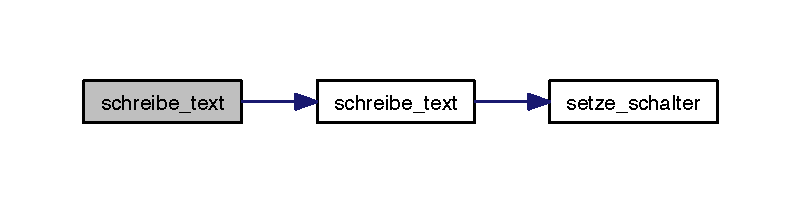
\includegraphics[width=350pt]{ausgabe_8cpp_a8124928a2d5ba8cb70d8368896ac6827_cgraph}
\end{center}
\end{figure}


\hypertarget{ausgabe_8cpp_a7b5a0354b89dacb17865e4735fea6a4f}{\index{ausgabe.\-cpp@{ausgabe.\-cpp}!schreibe\-\_\-text@{schreibe\-\_\-text}}
\index{schreibe\-\_\-text@{schreibe\-\_\-text}!ausgabe.cpp@{ausgabe.\-cpp}}
\subsubsection[{schreibe\-\_\-text}]{\setlength{\rightskip}{0pt plus 5cm}void schreibe\-\_\-text (
\begin{DoxyParamCaption}
\item[{string}]{text, }
\item[{streamsize}]{feldbreite}
\end{DoxyParamCaption}
)}}\label{ausgabe_8cpp_a7b5a0354b89dacb17865e4735fea6a4f}
Setzt verschiendene Schalter zu Steuerung und Formatierung der Ausgabe und schreibt einen Text auf den Bildschirm. 
\begin{DoxyParams}{Parameters}
{\em text} & Text der ausgegeben werden soll. \\
\hline
{\em feldbreite} & Feldbreite welche die Zahl haben soll. \\
\hline
\end{DoxyParams}


Definition at line 350 of file ausgabe.\-cpp.

\hypertarget{ausgabe_8cpp_aeded53f62c8030087f76c69a5e974918}{\index{ausgabe.\-cpp@{ausgabe.\-cpp}!schreibe\-\_\-text@{schreibe\-\_\-text}}
\index{schreibe\-\_\-text@{schreibe\-\_\-text}!ausgabe.cpp@{ausgabe.\-cpp}}
\subsubsection[{schreibe\-\_\-text}]{\setlength{\rightskip}{0pt plus 5cm}void schreibe\-\_\-text (
\begin{DoxyParamCaption}
\item[{string}]{text, }
\item[{streamsize}]{feldbreite, }
\item[{char}]{fuellzeichen}
\end{DoxyParamCaption}
)}}\label{ausgabe_8cpp_aeded53f62c8030087f76c69a5e974918}
Setzt verschiendene Schalter zu Steuerung und Formatierung der Ausgabe und schreibt einen Text auf den Bildschirm. 
\begin{DoxyParams}{Parameters}
{\em text} & Text der ausgegeben werden soll. \\
\hline
{\em feldbreite} & Feldbreite welche die Zahl haben soll. \\
\hline
{\em fuellzeichen} & Zeichen mit dem die restliche Feldbreite aufgefuellt werden soll. \\
\hline
\end{DoxyParams}


Definition at line 364 of file ausgabe.\-cpp.



Here is the call graph for this function\-:
\nopagebreak
\begin{figure}[H]
\begin{center}
\leavevmode
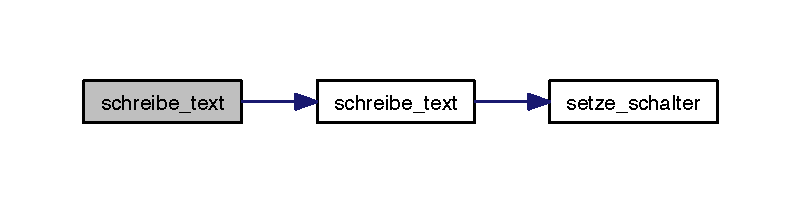
\includegraphics[width=350pt]{ausgabe_8cpp_aeded53f62c8030087f76c69a5e974918_cgraph}
\end{center}
\end{figure}


\hypertarget{ausgabe_8cpp_ab5931634ab2fd4e7863dd5be7d7f6b19}{\index{ausgabe.\-cpp@{ausgabe.\-cpp}!schreibe\-\_\-text@{schreibe\-\_\-text}}
\index{schreibe\-\_\-text@{schreibe\-\_\-text}!ausgabe.cpp@{ausgabe.\-cpp}}
\subsubsection[{schreibe\-\_\-text}]{\setlength{\rightskip}{0pt plus 5cm}void schreibe\-\_\-text (
\begin{DoxyParamCaption}
\item[{string}]{text, }
\item[{streamsize}]{feldbreite, }
\item[{ios\-\_\-base\-::fmtflags}]{format\mbox{[}$\,$\mbox{]}, }
\item[{int}]{anzahl\-\_\-formate}
\end{DoxyParamCaption}
)}}\label{ausgabe_8cpp_ab5931634ab2fd4e7863dd5be7d7f6b19}
Setzt verschiendene Schalter zu Steuerung und Formatierung der Ausgabe und schreibt einen Text auf den Bildschirm. 
\begin{DoxyParams}{Parameters}
{\em text} & Text der ausgegeben werden soll. \\
\hline
{\em feldbreite} & Feldbreite welche die Zahl haben soll. \\
\hline
{\em format} & Formatierung die vorgenommen werden soll. \\
\hline
{\em anzahl\-\_\-formate} & Formatierung die vorgenommen werden soll. \\
\hline
\end{DoxyParams}


Definition at line 379 of file ausgabe.\-cpp.



Here is the call graph for this function\-:
\nopagebreak
\begin{figure}[H]
\begin{center}
\leavevmode
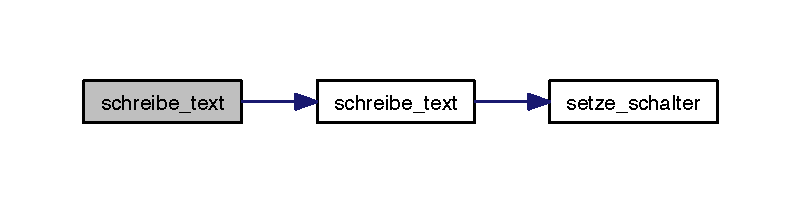
\includegraphics[width=350pt]{ausgabe_8cpp_ab5931634ab2fd4e7863dd5be7d7f6b19_cgraph}
\end{center}
\end{figure}


\hypertarget{ausgabe_8cpp_a2384f3389f4ad78d1c0f96058bef3024}{\index{ausgabe.\-cpp@{ausgabe.\-cpp}!schreibe\-\_\-text@{schreibe\-\_\-text}}
\index{schreibe\-\_\-text@{schreibe\-\_\-text}!ausgabe.cpp@{ausgabe.\-cpp}}
\subsubsection[{schreibe\-\_\-text}]{\setlength{\rightskip}{0pt plus 5cm}void schreibe\-\_\-text (
\begin{DoxyParamCaption}
\item[{string}]{text, }
\item[{streamsize}]{feldbreite, }
\item[{char}]{fuellzeichen, }
\item[{ios\-\_\-base\-::fmtflags}]{format\mbox{[}$\,$\mbox{]}, }
\item[{int}]{anzahl\-\_\-formate}
\end{DoxyParamCaption}
)}}\label{ausgabe_8cpp_a2384f3389f4ad78d1c0f96058bef3024}
Setzt verschiendene Schalter zu Steuerung und Formatierung der Ausgabe und schreibt einen Text auf den Bildschirm. 
\begin{DoxyParams}{Parameters}
{\em text} & Text der ausgegeben werden soll. \\
\hline
{\em feldbreite} & Feldbreite welche die Zahl haben soll. \\
\hline
{\em fuellzeichen} & Zeichen mit dem die restliche Feldbreite aufgefuellt werden soll. \\
\hline
{\em format} & Formatierung die vorgenommen werden soll. \\
\hline
{\em anzahl\-\_\-formate} & Formatierung die vorgenommen werden soll. \\
\hline
\end{DoxyParams}


Definition at line 395 of file ausgabe.\-cpp.



Here is the call graph for this function\-:
\nopagebreak
\begin{figure}[H]
\begin{center}
\leavevmode
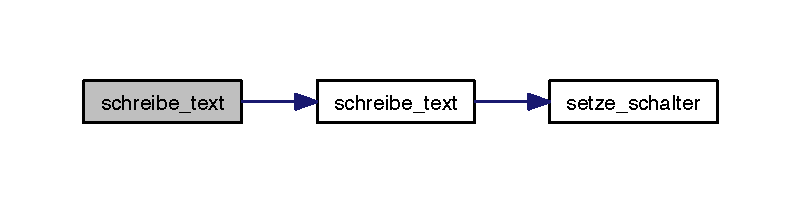
\includegraphics[width=350pt]{ausgabe_8cpp_a2384f3389f4ad78d1c0f96058bef3024_cgraph}
\end{center}
\end{figure}


\hypertarget{ausgabe_8cpp_a3109f9f4c65293eb538b2697fda647c9}{\index{ausgabe.\-cpp@{ausgabe.\-cpp}!schreibe\-\_\-zahl@{schreibe\-\_\-zahl}}
\index{schreibe\-\_\-zahl@{schreibe\-\_\-zahl}!ausgabe.cpp@{ausgabe.\-cpp}}
\subsubsection[{schreibe\-\_\-zahl}]{\setlength{\rightskip}{0pt plus 5cm}void schreibe\-\_\-zahl (
\begin{DoxyParamCaption}
\item[{long}]{zahl, }
\item[{ios\-\_\-base\-::fmtflags}]{format\mbox{[}$\,$\mbox{]}, }
\item[{int}]{anzahl\-\_\-formate}
\end{DoxyParamCaption}
)}}\label{ausgabe_8cpp_a3109f9f4c65293eb538b2697fda647c9}
Setzt verschiendene Schalter zu Steuerung und Formatierung der Ausgabe und schreibt eine Zahl auf den Bildschirm. 
\begin{DoxyParams}{Parameters}
{\em zahl} & Zahl die ausgegeben werden soll \\
\hline
{\em format} & Formatierung die Vorgenommen werden soll \\
\hline
{\em anzahl\-\_\-formate} & Formatierung die vorgenommen werden soll \\
\hline
\end{DoxyParams}


Definition at line 26 of file ausgabe.\-cpp.



Here is the call graph for this function\-:
\nopagebreak
\begin{figure}[H]
\begin{center}
\leavevmode
\includegraphics[width=274pt]{ausgabe_8cpp_a3109f9f4c65293eb538b2697fda647c9_cgraph}
\end{center}
\end{figure}




Here is the caller graph for this function\-:
\nopagebreak
\begin{figure}[H]
\begin{center}
\leavevmode
\includegraphics[width=350pt]{ausgabe_8cpp_a3109f9f4c65293eb538b2697fda647c9_icgraph}
\end{center}
\end{figure}


\hypertarget{ausgabe_8cpp_af597975886c508e6ad4449837c23b61e}{\index{ausgabe.\-cpp@{ausgabe.\-cpp}!schreibe\-\_\-zahl@{schreibe\-\_\-zahl}}
\index{schreibe\-\_\-zahl@{schreibe\-\_\-zahl}!ausgabe.cpp@{ausgabe.\-cpp}}
\subsubsection[{schreibe\-\_\-zahl}]{\setlength{\rightskip}{0pt plus 5cm}void schreibe\-\_\-zahl (
\begin{DoxyParamCaption}
\item[{long}]{zahl, }
\item[{ios\-\_\-base\-::fmtflags}]{format}
\end{DoxyParamCaption}
)}}\label{ausgabe_8cpp_af597975886c508e6ad4449837c23b61e}
Setzt verschiendene Schalter zu Steuerung und Formatierung der Ausgabe und schreibt eine Zahl auf den Bildschirm. 
\begin{DoxyParams}{Parameters}
{\em zahl} & Zahl die ausgegeben werden soll. \\
\hline
{\em format} & Formatierung die vorgenommen werden soll. \\
\hline
\end{DoxyParams}


Definition at line 61 of file ausgabe.\-cpp.



Here is the call graph for this function\-:
\nopagebreak
\begin{figure}[H]
\begin{center}
\leavevmode
\includegraphics[width=350pt]{ausgabe_8cpp_af597975886c508e6ad4449837c23b61e_cgraph}
\end{center}
\end{figure}


\hypertarget{ausgabe_8cpp_a9afeddc3a2e51a1d3c7e110fb16767cb}{\index{ausgabe.\-cpp@{ausgabe.\-cpp}!schreibe\-\_\-zahl@{schreibe\-\_\-zahl}}
\index{schreibe\-\_\-zahl@{schreibe\-\_\-zahl}!ausgabe.cpp@{ausgabe.\-cpp}}
\subsubsection[{schreibe\-\_\-zahl}]{\setlength{\rightskip}{0pt plus 5cm}void schreibe\-\_\-zahl (
\begin{DoxyParamCaption}
\item[{long}]{zahl, }
\item[{streamsize}]{feldbreite, }
\item[{ios\-\_\-base\-::fmtflags}]{format\mbox{[}$\,$\mbox{]}, }
\item[{int}]{anzahl\-\_\-formate}
\end{DoxyParamCaption}
)}}\label{ausgabe_8cpp_a9afeddc3a2e51a1d3c7e110fb16767cb}
Setzt verschiendene Schalter zu Steuerung und Formatierung der Ausgabe. und schreibt eine Zahl auf den Bildschirm. 
\begin{DoxyParams}{Parameters}
{\em zahl} & Zahl die ausgegeben werden soll. \\
\hline
{\em feldbreite} & welche die Zahl haben soll. \\
\hline
{\em format} & Formatierung die vorgenommen werden soll. \\
\hline
{\em anzahl\-\_\-formate} & Formatierung die vorgenommen werden soll. \\
\hline
\end{DoxyParams}


Definition at line 74 of file ausgabe.\-cpp.



Here is the call graph for this function\-:
\nopagebreak
\begin{figure}[H]
\begin{center}
\leavevmode
\includegraphics[width=350pt]{ausgabe_8cpp_a9afeddc3a2e51a1d3c7e110fb16767cb_cgraph}
\end{center}
\end{figure}


\hypertarget{ausgabe_8cpp_a0381140ca142dea69e5e466a45d8982c}{\index{ausgabe.\-cpp@{ausgabe.\-cpp}!schreibe\-\_\-zahl@{schreibe\-\_\-zahl}}
\index{schreibe\-\_\-zahl@{schreibe\-\_\-zahl}!ausgabe.cpp@{ausgabe.\-cpp}}
\subsubsection[{schreibe\-\_\-zahl}]{\setlength{\rightskip}{0pt plus 5cm}void schreibe\-\_\-zahl (
\begin{DoxyParamCaption}
\item[{long}]{zahl, }
\item[{streamsize}]{feldbreite, }
\item[{ios\-\_\-base\-::fmtflags}]{format}
\end{DoxyParamCaption}
)}}\label{ausgabe_8cpp_a0381140ca142dea69e5e466a45d8982c}
Schreibt eine Zahl mit bestimmten Foramtierungen. 
\begin{DoxyParams}{Parameters}
{\em zahl} & Zahl die ausgegeben werden soll. \\
\hline
{\em feldbreite} & Feldbreite mit dem der Wert ausgegeben werden soll. \\
\hline
{\em format} & Formatierung die Vorgenommen werden soll. \\
\hline
\end{DoxyParams}


Definition at line 87 of file ausgabe.\-cpp.



Here is the call graph for this function\-:
\nopagebreak
\begin{figure}[H]
\begin{center}
\leavevmode
\includegraphics[width=350pt]{ausgabe_8cpp_a0381140ca142dea69e5e466a45d8982c_cgraph}
\end{center}
\end{figure}


\hypertarget{ausgabe_8cpp_ad67b1282696f63e5b34b1647d274077f}{\index{ausgabe.\-cpp@{ausgabe.\-cpp}!schreibe\-\_\-zahl@{schreibe\-\_\-zahl}}
\index{schreibe\-\_\-zahl@{schreibe\-\_\-zahl}!ausgabe.cpp@{ausgabe.\-cpp}}
\subsubsection[{schreibe\-\_\-zahl}]{\setlength{\rightskip}{0pt plus 5cm}void schreibe\-\_\-zahl (
\begin{DoxyParamCaption}
\item[{long}]{zahl, }
\item[{streamsize}]{feldbreite, }
\item[{char}]{fuellzeichen, }
\item[{ios\-\_\-base\-::fmtflags}]{format\mbox{[}$\,$\mbox{]}, }
\item[{int}]{anzahl\-\_\-formate}
\end{DoxyParamCaption}
)}}\label{ausgabe_8cpp_ad67b1282696f63e5b34b1647d274077f}
Setzt verschiendene Schalter zu Steuerung und Formatierung der Ausgabe. und schreibt eine Zahl auf den Bildschirm. 
\begin{DoxyParams}{Parameters}
{\em zahl} & Zahl die ausgegeben werden soll. \\
\hline
{\em feldbreite} & Feldbreite welche die Zahl haben soll. \\
\hline
{\em fuellzeichen} & Zeichen mit dem die restliche Feldbreite aufgefuellt werden soll. \\
\hline
{\em format} & Formatierung die vorgenommen werden soll. \\
\hline
{\em anzahl\-\_\-formate} & Formatierung die vorgenommen werden soll. \\
\hline
\end{DoxyParams}


Definition at line 101 of file ausgabe.\-cpp.



Here is the call graph for this function\-:
\nopagebreak
\begin{figure}[H]
\begin{center}
\leavevmode
\includegraphics[width=350pt]{ausgabe_8cpp_ad67b1282696f63e5b34b1647d274077f_cgraph}
\end{center}
\end{figure}


\hypertarget{ausgabe_8cpp_a1665a46b00999bb8a0aca574ed0ed827}{\index{ausgabe.\-cpp@{ausgabe.\-cpp}!schreibe\-\_\-zahl@{schreibe\-\_\-zahl}}
\index{schreibe\-\_\-zahl@{schreibe\-\_\-zahl}!ausgabe.cpp@{ausgabe.\-cpp}}
\subsubsection[{schreibe\-\_\-zahl}]{\setlength{\rightskip}{0pt plus 5cm}void schreibe\-\_\-zahl (
\begin{DoxyParamCaption}
\item[{long}]{zahl, }
\item[{streamsize}]{feldbreite, }
\item[{char}]{fuellzeichen, }
\item[{ios\-\_\-base\-::fmtflags}]{format}
\end{DoxyParamCaption}
)}}\label{ausgabe_8cpp_a1665a46b00999bb8a0aca574ed0ed827}
Setzt verschiendene Schalter zu Steuerung und Formatierung der Ausgabe. und schreibt eine Zahl auf den Bildschirm. 
\begin{DoxyParams}{Parameters}
{\em zahl} & Zahl die ausgegeben werden soll. \\
\hline
{\em feldbreite} & Feldbreite welche die Zahl haben soll. \\
\hline
{\em fuellzeichen} & Zeichen mit dem die restliche Feldbreite aufgefuellt werden soll. \\
\hline
{\em format} & Formatierung die vorgenommen werden soll. \\
\hline
\end{DoxyParams}


Definition at line 116 of file ausgabe.\-cpp.



Here is the call graph for this function\-:
\nopagebreak
\begin{figure}[H]
\begin{center}
\leavevmode
\includegraphics[width=350pt]{ausgabe_8cpp_a1665a46b00999bb8a0aca574ed0ed827_cgraph}
\end{center}
\end{figure}


\hypertarget{ausgabe_8cpp_ad428331d8837c1f886c98d996defa4c0}{\index{ausgabe.\-cpp@{ausgabe.\-cpp}!schreibe\-\_\-zahl@{schreibe\-\_\-zahl}}
\index{schreibe\-\_\-zahl@{schreibe\-\_\-zahl}!ausgabe.cpp@{ausgabe.\-cpp}}
\subsubsection[{schreibe\-\_\-zahl}]{\setlength{\rightskip}{0pt plus 5cm}void schreibe\-\_\-zahl (
\begin{DoxyParamCaption}
\item[{long double}]{zahl, }
\item[{ios\-\_\-base\-::fmtflags}]{format\mbox{[}$\,$\mbox{]}, }
\item[{int}]{anzahl\-\_\-formate}
\end{DoxyParamCaption}
)}}\label{ausgabe_8cpp_ad428331d8837c1f886c98d996defa4c0}
Setzt verschiendene Schalter zu Steuerung und Formatierung der Ausgabe und schreibt eine Zahl auf den Bildschirm. 
\begin{DoxyParams}{Parameters}
{\em zahl} & Zahl die ausgegeben werden soll. \\
\hline
{\em format} & Formatierung die vorgenommen werden soll. \\
\hline
{\em anzahl\-\_\-formate} & Formatierung die vorgenommen werden soll. \\
\hline
\end{DoxyParams}


Definition at line 128 of file ausgabe.\-cpp.



Here is the call graph for this function\-:
\nopagebreak
\begin{figure}[H]
\begin{center}
\leavevmode
\includegraphics[width=274pt]{ausgabe_8cpp_ad428331d8837c1f886c98d996defa4c0_cgraph}
\end{center}
\end{figure}


\hypertarget{ausgabe_8cpp_af641fdccfc7fc8e61718fb3638e527e7}{\index{ausgabe.\-cpp@{ausgabe.\-cpp}!schreibe\-\_\-zahl@{schreibe\-\_\-zahl}}
\index{schreibe\-\_\-zahl@{schreibe\-\_\-zahl}!ausgabe.cpp@{ausgabe.\-cpp}}
\subsubsection[{schreibe\-\_\-zahl}]{\setlength{\rightskip}{0pt plus 5cm}void schreibe\-\_\-zahl (
\begin{DoxyParamCaption}
\item[{long double}]{zahl, }
\item[{ios\-\_\-base\-::fmtflags}]{format}
\end{DoxyParamCaption}
)}}\label{ausgabe_8cpp_af641fdccfc7fc8e61718fb3638e527e7}
Setzt verschiendene Schalter zu Steuerung und Formatierung der Ausgabe und schreibt eine Zahl auf den Bildschirm. 
\begin{DoxyParams}{Parameters}
{\em zahl} & Zahl die ausgegeben werden soll. \\
\hline
{\em format} & Formatierung die vorgenommen werden soll. \\
\hline
\end{DoxyParams}


Definition at line 142 of file ausgabe.\-cpp.



Here is the call graph for this function\-:
\nopagebreak
\begin{figure}[H]
\begin{center}
\leavevmode
\includegraphics[width=350pt]{ausgabe_8cpp_af641fdccfc7fc8e61718fb3638e527e7_cgraph}
\end{center}
\end{figure}


\hypertarget{ausgabe_8cpp_a990c6f1274271b12da060a298a97412d}{\index{ausgabe.\-cpp@{ausgabe.\-cpp}!schreibe\-\_\-zahl@{schreibe\-\_\-zahl}}
\index{schreibe\-\_\-zahl@{schreibe\-\_\-zahl}!ausgabe.cpp@{ausgabe.\-cpp}}
\subsubsection[{schreibe\-\_\-zahl}]{\setlength{\rightskip}{0pt plus 5cm}void schreibe\-\_\-zahl (
\begin{DoxyParamCaption}
\item[{long double}]{zahl, }
\item[{streamsize}]{feldbreite, }
\item[{ios\-\_\-base\-::fmtflags}]{format\mbox{[}$\,$\mbox{]}, }
\item[{int}]{anzahl\-\_\-formate}
\end{DoxyParamCaption}
)}}\label{ausgabe_8cpp_a990c6f1274271b12da060a298a97412d}
Setzt verschiendene Schalter zu Steuerung und Formatierung der Ausgabe und schreibt eine Zahl auf den Bildschirm. 
\begin{DoxyParams}{Parameters}
{\em zahl} & Zahl die ausgegeben werden soll. \\
\hline
{\em feldbreite} & Feldbreite welche die Zahl haben soll. \\
\hline
{\em format} & Formatierung die vorgenommen werden soll. \\
\hline
{\em anzahl\-\_\-formate} & Formatierung die vorgenommen werden soll. \\
\hline
\end{DoxyParams}


Definition at line 155 of file ausgabe.\-cpp.



Here is the call graph for this function\-:
\nopagebreak
\begin{figure}[H]
\begin{center}
\leavevmode
\includegraphics[width=350pt]{ausgabe_8cpp_a990c6f1274271b12da060a298a97412d_cgraph}
\end{center}
\end{figure}


\hypertarget{ausgabe_8cpp_a34b32ea150b542c42bd16e8d74832f43}{\index{ausgabe.\-cpp@{ausgabe.\-cpp}!schreibe\-\_\-zahl@{schreibe\-\_\-zahl}}
\index{schreibe\-\_\-zahl@{schreibe\-\_\-zahl}!ausgabe.cpp@{ausgabe.\-cpp}}
\subsubsection[{schreibe\-\_\-zahl}]{\setlength{\rightskip}{0pt plus 5cm}void schreibe\-\_\-zahl (
\begin{DoxyParamCaption}
\item[{long double}]{zahl, }
\item[{streamsize}]{feldbreite, }
\item[{ios\-\_\-base\-::fmtflags}]{format}
\end{DoxyParamCaption}
)}}\label{ausgabe_8cpp_a34b32ea150b542c42bd16e8d74832f43}
Setzt verschiendene Schalter zu Steuerung und Formatierung der Ausgabe und schreibt eine Gleitkommazahl auf den Bildschirm. 
\begin{DoxyParams}{Parameters}
{\em zahl} & Zahl die ausgegeben werden soll. \\
\hline
{\em feldbreite} & Feldbreite welche die Zahl haben soll. \\
\hline
{\em format} & Formatierung die vorgenommen werden soll. \\
\hline
\end{DoxyParams}


Definition at line 169 of file ausgabe.\-cpp.



Here is the call graph for this function\-:
\nopagebreak
\begin{figure}[H]
\begin{center}
\leavevmode
\includegraphics[width=350pt]{ausgabe_8cpp_a34b32ea150b542c42bd16e8d74832f43_cgraph}
\end{center}
\end{figure}


\hypertarget{ausgabe_8cpp_a7b6c3648ab9f0080c79ecb8aae689a0d}{\index{ausgabe.\-cpp@{ausgabe.\-cpp}!schreibe\-\_\-zahl@{schreibe\-\_\-zahl}}
\index{schreibe\-\_\-zahl@{schreibe\-\_\-zahl}!ausgabe.cpp@{ausgabe.\-cpp}}
\subsubsection[{schreibe\-\_\-zahl}]{\setlength{\rightskip}{0pt plus 5cm}void schreibe\-\_\-zahl (
\begin{DoxyParamCaption}
\item[{long double}]{zahl, }
\item[{streamsize}]{feldbreite, }
\item[{char}]{fuellzeichen, }
\item[{ios\-\_\-base\-::fmtflags}]{format\mbox{[}$\,$\mbox{]}, }
\item[{int}]{anzahl\-\_\-formate}
\end{DoxyParamCaption}
)}}\label{ausgabe_8cpp_a7b6c3648ab9f0080c79ecb8aae689a0d}
Setzt verschiendene Schalter zu Steuerung und Formatierung der Ausgabe und schreibt eine Gleitkommazahl auf den Bildschirm. 
\begin{DoxyParams}{Parameters}
{\em zahl} & Zahl die ausgegeben werden soll. \\
\hline
{\em feldbreite} & Feldbreite welche die Zahl haben soll. \\
\hline
{\em fuellzeichen} & Zeichen mit dem die restliche Feldbreite aufgefuellt werden soll. \\
\hline
{\em format} & Formatierung die vorgenommen werden soll. \\
\hline
{\em anzahl\-\_\-formate} & Formatierung die vorgenommen werden soll. \\
\hline
\end{DoxyParams}


Definition at line 183 of file ausgabe.\-cpp.



Here is the call graph for this function\-:
\nopagebreak
\begin{figure}[H]
\begin{center}
\leavevmode
\includegraphics[width=350pt]{ausgabe_8cpp_a7b6c3648ab9f0080c79ecb8aae689a0d_cgraph}
\end{center}
\end{figure}


\hypertarget{ausgabe_8cpp_a7ee381ed414a7c21377514a823b3eb33}{\index{ausgabe.\-cpp@{ausgabe.\-cpp}!schreibe\-\_\-zahl@{schreibe\-\_\-zahl}}
\index{schreibe\-\_\-zahl@{schreibe\-\_\-zahl}!ausgabe.cpp@{ausgabe.\-cpp}}
\subsubsection[{schreibe\-\_\-zahl}]{\setlength{\rightskip}{0pt plus 5cm}void schreibe\-\_\-zahl (
\begin{DoxyParamCaption}
\item[{long double}]{zahl, }
\item[{streamsize}]{feldbreite, }
\item[{char}]{fuellzeichen, }
\item[{ios\-\_\-base\-::fmtflags}]{format\mbox{[}$\,$\mbox{]}, }
\item[{int}]{anzahl\-\_\-formate, }
\item[{streamsize}]{praezision}
\end{DoxyParamCaption}
)}}\label{ausgabe_8cpp_a7ee381ed414a7c21377514a823b3eb33}
Setzt verschiendene Schalter zu Steuerung und Formatierung der Ausgabe und schreibt eine Gleitkommazahl auf den Bildschirm. 
\begin{DoxyParams}{Parameters}
{\em zahl} & Zahl die ausgegeben werden soll. \\
\hline
{\em feldbreite} & Feldbreite welche die Zahl haben soll. \\
\hline
{\em fuellzeichen} & Zeichen mit dem die restliche Feldbreite aufgefuellt werden soll. \\
\hline
{\em format} & Formatierung die vorgenommen werden soll. \\
\hline
{\em anzahl\-\_\-formate} & Formatierung die vorgenommen werden soll. \\
\hline
{\em praezision} & Praezision der Gleitkommazahl \\
\hline
\end{DoxyParams}


Definition at line 200 of file ausgabe.\-cpp.



Here is the call graph for this function\-:
\nopagebreak
\begin{figure}[H]
\begin{center}
\leavevmode
\includegraphics[width=350pt]{ausgabe_8cpp_a7ee381ed414a7c21377514a823b3eb33_cgraph}
\end{center}
\end{figure}


\hypertarget{ausgabe_8cpp_a9b4a59d38449fe87419fb125fc63ed93}{\index{ausgabe.\-cpp@{ausgabe.\-cpp}!schreibe\-\_\-zahl@{schreibe\-\_\-zahl}}
\index{schreibe\-\_\-zahl@{schreibe\-\_\-zahl}!ausgabe.cpp@{ausgabe.\-cpp}}
\subsubsection[{schreibe\-\_\-zahl}]{\setlength{\rightskip}{0pt plus 5cm}void schreibe\-\_\-zahl (
\begin{DoxyParamCaption}
\item[{double}]{zahl, }
\item[{streamsize}]{feldbreite, }
\item[{char}]{fuellzeichen, }
\item[{ios\-\_\-base\-::fmtflags}]{format\mbox{[}$\,$\mbox{]}, }
\item[{int}]{anzahl\-\_\-formate}
\end{DoxyParamCaption}
)}}\label{ausgabe_8cpp_a9b4a59d38449fe87419fb125fc63ed93}
Setzt verschiendene Schalter zu Steuerung und Formatierung der Ausgabe und schreibt eine Gleitkommazahl auf den Bildschirm. 
\begin{DoxyParams}{Parameters}
{\em zahl} & Zahl die ausgegeben werden soll. \\
\hline
{\em feldbreite} & Feldbreite welche die Zahl haben soll. \\
\hline
{\em fuellzeichen} & Zeichen mit dem die restliche Feldbreite aufgefuellt werden soll. \\
\hline
{\em format} & Formatierung die vorgenommen werden soll. \\
\hline
{\em anzahl\-\_\-formate} & Formatierung die vorgenommen werden soll. \\
\hline
\end{DoxyParams}


Definition at line 215 of file ausgabe.\-cpp.



Here is the call graph for this function\-:
\nopagebreak
\begin{figure}[H]
\begin{center}
\leavevmode
\includegraphics[width=350pt]{ausgabe_8cpp_a9b4a59d38449fe87419fb125fc63ed93_cgraph}
\end{center}
\end{figure}


\hypertarget{ausgabe_8cpp_a5b12b6a0fe6cc5d43f63e6f72b1b2d45}{\index{ausgabe.\-cpp@{ausgabe.\-cpp}!schreibe\-\_\-zahl@{schreibe\-\_\-zahl}}
\index{schreibe\-\_\-zahl@{schreibe\-\_\-zahl}!ausgabe.cpp@{ausgabe.\-cpp}}
\subsubsection[{schreibe\-\_\-zahl}]{\setlength{\rightskip}{0pt plus 5cm}void schreibe\-\_\-zahl (
\begin{DoxyParamCaption}
\item[{int}]{zahl, }
\item[{streamsize}]{feldbreite, }
\item[{char}]{fuellzeichen, }
\item[{ios\-\_\-base\-::fmtflags}]{format\mbox{[}$\,$\mbox{]}, }
\item[{int}]{anzahl\-\_\-formate}
\end{DoxyParamCaption}
)}}\label{ausgabe_8cpp_a5b12b6a0fe6cc5d43f63e6f72b1b2d45}
Setzt verschiendene Schalter zu Steuerung und Formatierung der Ausgabe und schreibt eine Gleitkommazahl auf den Bildschirm. 
\begin{DoxyParams}{Parameters}
{\em zahl} & Zahl die ausgegeben werden soll. \\
\hline
{\em feldbreite} & Feldbreite welche die Zahl haben soll. \\
\hline
{\em fuellzeichen} & Zeichen mit dem die restliche Feldbreite aufgefuellt werden soll. \\
\hline
{\em format} & Formatierung die vorgenommen werden soll. \\
\hline
{\em anzahl\-\_\-formate} & Formatierung die vorgenommen werden soll. \\
\hline
\end{DoxyParams}


Definition at line 227 of file ausgabe.\-cpp.



Here is the call graph for this function\-:
\nopagebreak
\begin{figure}[H]
\begin{center}
\leavevmode
\includegraphics[width=350pt]{ausgabe_8cpp_a5b12b6a0fe6cc5d43f63e6f72b1b2d45_cgraph}
\end{center}
\end{figure}


\hypertarget{ausgabe_8cpp_abf47c230eab9d30163dd908e4a1f65e7}{\index{ausgabe.\-cpp@{ausgabe.\-cpp}!schreibe\-\_\-zahl@{schreibe\-\_\-zahl}}
\index{schreibe\-\_\-zahl@{schreibe\-\_\-zahl}!ausgabe.cpp@{ausgabe.\-cpp}}
\subsubsection[{schreibe\-\_\-zahl}]{\setlength{\rightskip}{0pt plus 5cm}void schreibe\-\_\-zahl (
\begin{DoxyParamCaption}
\item[{long double}]{zahl, }
\item[{streamsize}]{feldbreite, }
\item[{char}]{fuellzeichen, }
\item[{ios\-\_\-base\-::fmtflags}]{format}
\end{DoxyParamCaption}
)}}\label{ausgabe_8cpp_abf47c230eab9d30163dd908e4a1f65e7}
Setzt verschiendene Schalter zu Steuerung und Formatierung der Ausgabe und schreibt eine Gleitkommazahl auf den Bildschirm. 
\begin{DoxyParams}{Parameters}
{\em zahl} & Zahl die ausgegeben werden soll. \\
\hline
{\em feldbreite} & Feldbreite welche die Zahl haben soll. \\
\hline
{\em fuellzeichen} & Zeichen mit dem die restliche Feldbreite aufgefuellt werden soll. \\
\hline
{\em format} & Formatierung die vorgenommen werden soll. \\
\hline
\end{DoxyParams}


Definition at line 239 of file ausgabe.\-cpp.



Here is the call graph for this function\-:
\nopagebreak
\begin{figure}[H]
\begin{center}
\leavevmode
\includegraphics[width=350pt]{ausgabe_8cpp_abf47c230eab9d30163dd908e4a1f65e7_cgraph}
\end{center}
\end{figure}


\hypertarget{ausgabe_8cpp_aed6b39beca8a03fa3143258918f6253e}{\index{ausgabe.\-cpp@{ausgabe.\-cpp}!schreibe\-\_\-zahl@{schreibe\-\_\-zahl}}
\index{schreibe\-\_\-zahl@{schreibe\-\_\-zahl}!ausgabe.cpp@{ausgabe.\-cpp}}
\subsubsection[{schreibe\-\_\-zahl}]{\setlength{\rightskip}{0pt plus 5cm}void schreibe\-\_\-zahl (
\begin{DoxyParamCaption}
\item[{streamsize}]{praezision, }
\item[{long double}]{zahl, }
\item[{streamsize}]{feldbreite, }
\item[{ios\-\_\-base\-::fmtflags}]{format\mbox{[}$\,$\mbox{]}, }
\item[{int}]{anzahl\-\_\-formate}
\end{DoxyParamCaption}
)}}\label{ausgabe_8cpp_aed6b39beca8a03fa3143258918f6253e}
Setzt verschiendene Schalter zu Steuerung und Formatierung der Ausgabe und schreibt eine Gleitkommazahl auf den Bildschirm. 
\begin{DoxyParams}{Parameters}
{\em praezision} & Praezision der Gleitkommazahl \\
\hline
{\em zahl} & Zahl die ausgegeben werden soll. \\
\hline
{\em feldbreite} & Feldbreite welche die Zahl haben soll. \\
\hline
{\em format} & Formatierung die vorgenommen werden soll. \\
\hline
{\em anzahl\-\_\-formate} & Formatierung die vorgenommen werden soll. \\
\hline
\end{DoxyParams}


Definition at line 253 of file ausgabe.\-cpp.



Here is the call graph for this function\-:
\nopagebreak
\begin{figure}[H]
\begin{center}
\leavevmode
\includegraphics[width=350pt]{ausgabe_8cpp_aed6b39beca8a03fa3143258918f6253e_cgraph}
\end{center}
\end{figure}


\hypertarget{ausgabe_8cpp_ae8c346aa92fc891022a940f2c5c75f95}{\index{ausgabe.\-cpp@{ausgabe.\-cpp}!setze\-\_\-schalter@{setze\-\_\-schalter}}
\index{setze\-\_\-schalter@{setze\-\_\-schalter}!ausgabe.cpp@{ausgabe.\-cpp}}
\subsubsection[{setze\-\_\-schalter}]{\setlength{\rightskip}{0pt plus 5cm}void setze\-\_\-schalter (
\begin{DoxyParamCaption}
\item[{ios\-\_\-base\-::fmtflags}]{format}
\end{DoxyParamCaption}
)}}\label{ausgabe_8cpp_ae8c346aa92fc891022a940f2c5c75f95}
Setzt verschiendene Schalter zu Steuerung und Formatierung der Ausgabe 
\begin{DoxyParams}{Parameters}
{\em format} & Formatierung die Vorgenommen werden soll \\
\hline
\end{DoxyParams}


Definition at line 6 of file ausgabe.\-cpp.



Here is the caller graph for this function\-:
\nopagebreak
\begin{figure}[H]
\begin{center}
\leavevmode
\includegraphics[width=350pt]{ausgabe_8cpp_ae8c346aa92fc891022a940f2c5c75f95_icgraph}
\end{center}
\end{figure}


\hypertarget{ausgabe_8cpp_abb46ef5c5d536396f1baa9c1a6ce1ccd}{\index{ausgabe.\-cpp@{ausgabe.\-cpp}!spaltenvorschub@{spaltenvorschub}}
\index{spaltenvorschub@{spaltenvorschub}!ausgabe.cpp@{ausgabe.\-cpp}}
\subsubsection[{spaltenvorschub}]{\setlength{\rightskip}{0pt plus 5cm}void spaltenvorschub (
\begin{DoxyParamCaption}
\item[{streamsize}]{feldbreite}
\end{DoxyParamCaption}
)}}\label{ausgabe_8cpp_abb46ef5c5d536396f1baa9c1a6ce1ccd}
Macht einene Spaltenvorschub um die Uebergebene laenge. 
\begin{DoxyParams}{Parameters}
{\em feldbreite} & Feldbreite ganzzzahliger datentyp der einen Spaltenvorschub um den entsprechenden Wert macht \\
\hline
\end{DoxyParams}


Definition at line 288 of file ausgabe.\-cpp.

\hypertarget{ausgabe_8cpp_aa3b21853f890838c88d047d6c2786917}{\index{ausgabe.\-cpp@{ausgabe.\-cpp}!wait@{wait}}
\index{wait@{wait}!ausgabe.cpp@{ausgabe.\-cpp}}
\subsubsection[{wait}]{\setlength{\rightskip}{0pt plus 5cm}void wait (
\begin{DoxyParamCaption}
{}
\end{DoxyParamCaption}
)}}\label{ausgabe_8cpp_aa3b21853f890838c88d047d6c2786917}
Haelt das Programm an nach druecken einer beliebigen Taste wird es fortgefuehrt. 

Definition at line 404 of file ausgabe.\-cpp.

\hypertarget{ausgabe_8cpp_a3737ce85b2d24f69b0960cebb26bea22}{\index{ausgabe.\-cpp@{ausgabe.\-cpp}!zeige\-\_\-zahl@{zeige\-\_\-zahl}}
\index{zeige\-\_\-zahl@{zeige\-\_\-zahl}!ausgabe.cpp@{ausgabe.\-cpp}}
\subsubsection[{zeige\-\_\-zahl}]{\setlength{\rightskip}{0pt plus 5cm}void zeige\-\_\-zahl (
\begin{DoxyParamCaption}
\item[{double}]{wert, }
\item[{streamsize}]{praezision}
\end{DoxyParamCaption}
)}}\label{ausgabe_8cpp_a3737ce85b2d24f69b0960cebb26bea22}
Dient der Ausgabe einer Gleitkommazahl mit entsprechender Praezision. 
\begin{DoxyParams}{Parameters}
{\em wert} & Wert der ausgegeben werden soll. \\
\hline
{\em praezision} & Praezision die verwendet werden soll. \\
\hline
\end{DoxyParams}


Definition at line 278 of file ausgabe.\-cpp.



Here is the call graph for this function\-:
\nopagebreak
\begin{figure}[H]
\begin{center}
\leavevmode
\includegraphics[width=350pt]{ausgabe_8cpp_a3737ce85b2d24f69b0960cebb26bea22_cgraph}
\end{center}
\end{figure}




Here is the caller graph for this function\-:
\nopagebreak
\begin{figure}[H]
\begin{center}
\leavevmode
\includegraphics[width=350pt]{ausgabe_8cpp_a3737ce85b2d24f69b0960cebb26bea22_icgraph}
\end{center}
\end{figure}


\hypertarget{ausgabe_8cpp_ace96c319620ef24d874ccb41b42601f3}{\index{ausgabe.\-cpp@{ausgabe.\-cpp}!zeige\-\_\-zahl\-\_\-von\-\_\-bis@{zeige\-\_\-zahl\-\_\-von\-\_\-bis}}
\index{zeige\-\_\-zahl\-\_\-von\-\_\-bis@{zeige\-\_\-zahl\-\_\-von\-\_\-bis}!ausgabe.cpp@{ausgabe.\-cpp}}
\subsubsection[{zeige\-\_\-zahl\-\_\-von\-\_\-bis}]{\setlength{\rightskip}{0pt plus 5cm}void zeige\-\_\-zahl\-\_\-von\-\_\-bis (
\begin{DoxyParamCaption}
\item[{long double}]{von, }
\item[{long double}]{bis, }
\item[{long double}]{abstand, }
\item[{streamsize}]{praezision}
\end{DoxyParamCaption}
)}}\label{ausgabe_8cpp_ace96c319620ef24d874ccb41b42601f3}
Zeigt die Zahlen aus einem Bereich mit einem definierten abstand und schreibt eine Gleitkommazahl auf den Bildschirm. 
\begin{DoxyParams}{Parameters}
{\em von} & Anfang des Bereiches. \\
\hline
{\em bis} & Ende des Bereiches. \\
\hline
{\em abstand} & Abstand in dem die Zahl ausgegeben werden soll. \\
\hline
{\em praezision} & Praezision der Gleitkommazahl \\
\hline
\end{DoxyParams}


Definition at line 268 of file ausgabe.\-cpp.



Here is the call graph for this function\-:
\nopagebreak
\begin{figure}[H]
\begin{center}
\leavevmode
\includegraphics[width=350pt]{ausgabe_8cpp_ace96c319620ef24d874ccb41b42601f3_cgraph}
\end{center}
\end{figure}



\hypertarget{ausgabe_8h}{\section{helper/ausgabe.h File Reference}
\label{ausgabe_8h}\index{helper/ausgabe.\-h@{helper/ausgabe.\-h}}
}
{\ttfamily \#include $<$cstdlib$>$}\\*
{\ttfamily \#include $<$iostream$>$}\\*
{\ttfamily \#include $<$stdio.\-h$>$}\\*
{\ttfamily \#include $<$sstream$>$}\\*
Include dependency graph for ausgabe.\-h\-:
\nopagebreak
\begin{figure}[H]
\begin{center}
\leavevmode
\includegraphics[width=329pt]{ausgabe_8h__incl}
\end{center}
\end{figure}
This graph shows which files directly or indirectly include this file\-:
\nopagebreak
\begin{figure}[H]
\begin{center}
\leavevmode
\includegraphics[width=343pt]{ausgabe_8h__dep__incl}
\end{center}
\end{figure}
\subsection*{Macros}
\begin{DoxyCompactItemize}
\item 
\#define \hyperlink{ausgabe_8h_ada0430ff0133c72d1ab38ca336610f5a}{clrscr}()~printf(\char`\"{}clrscr() -\/ Fehler!\textbackslash{}n\char`\"{})
\end{DoxyCompactItemize}
\subsection*{Typedefs}
\begin{DoxyCompactItemize}
\item 
typedef ios\-\_\-base\-::fmtflags \hyperlink{ausgabe_8h_af955de3b073f1d8d6ef467ddb60837b9}{Formattyp}
\end{DoxyCompactItemize}
\subsection*{Functions}
\begin{DoxyCompactItemize}
\item 
void \hyperlink{ausgabe_8h_a83c6a2f7b4a96e0c20b2119f3960022d}{loesche\-\_\-bildschirm} ()
\item 
void \hyperlink{ausgabe_8h_a5db6071f8d9d29f5e775bb27d50480a4}{loesche\-\_\-bildschirm\-\_\-mit\-\_\-header} ()
\item 
void \hyperlink{ausgabe_8h_a42662dc47ec6886db83f4fa886f87e32}{header} ()
\item 
void \hyperlink{ausgabe_8h_ae8c346aa92fc891022a940f2c5c75f95}{setze\-\_\-schalter} (ios\-\_\-base\-::fmtflags format)
\item 
void \hyperlink{ausgabe_8h_a3109f9f4c65293eb538b2697fda647c9}{schreibe\-\_\-zahl} (long zahl, ios\-\_\-base\-::fmtflags format\mbox{[}$\,$\mbox{]}, int anzahl\-\_\-formate)
\item 
void \hyperlink{ausgabe_8h_af597975886c508e6ad4449837c23b61e}{schreibe\-\_\-zahl} (long zahl, ios\-\_\-base\-::fmtflags format)
\item 
void \hyperlink{ausgabe_8h_a9afeddc3a2e51a1d3c7e110fb16767cb}{schreibe\-\_\-zahl} (long zahl, streamsize feldbreite, ios\-\_\-base\-::fmtflags format\mbox{[}$\,$\mbox{]}, int anzahl\-\_\-formate)
\item 
void \hyperlink{ausgabe_8h_a0381140ca142dea69e5e466a45d8982c}{schreibe\-\_\-zahl} (long zahl, streamsize feldbreite, ios\-\_\-base\-::fmtflags format)
\item 
void \hyperlink{ausgabe_8h_ad67b1282696f63e5b34b1647d274077f}{schreibe\-\_\-zahl} (long zahl, streamsize feldbreite, char fuellzeichen, ios\-\_\-base\-::fmtflags format\mbox{[}$\,$\mbox{]}, int anzahl\-\_\-formate)
\item 
void \hyperlink{ausgabe_8h_a1665a46b00999bb8a0aca574ed0ed827}{schreibe\-\_\-zahl} (long zahl, streamsize feldbreite, char fuellzeichen, ios\-\_\-base\-::fmtflags format)
\item 
void \hyperlink{ausgabe_8h_ad428331d8837c1f886c98d996defa4c0}{schreibe\-\_\-zahl} (long double zahl, ios\-\_\-base\-::fmtflags format\mbox{[}$\,$\mbox{]}, int anzahl\-\_\-formate)
\item 
void \hyperlink{ausgabe_8h_af641fdccfc7fc8e61718fb3638e527e7}{schreibe\-\_\-zahl} (long double zahl, ios\-\_\-base\-::fmtflags format)
\item 
void \hyperlink{ausgabe_8h_a34b32ea150b542c42bd16e8d74832f43}{schreibe\-\_\-zahl} (long double zahl, streamsize feldbreite, ios\-\_\-base\-::fmtflags format)
\item 
void \hyperlink{ausgabe_8h_a7b6c3648ab9f0080c79ecb8aae689a0d}{schreibe\-\_\-zahl} (long double zahl, streamsize feldbreite, char fuellzeichen, ios\-\_\-base\-::fmtflags format\mbox{[}$\,$\mbox{]}, int anzahl\-\_\-formate)
\item 
void \hyperlink{ausgabe_8h_a7ee381ed414a7c21377514a823b3eb33}{schreibe\-\_\-zahl} (long double zahl, streamsize feldbreite, char fuellzeichen, ios\-\_\-base\-::fmtflags format\mbox{[}$\,$\mbox{]}, int anzahl\-\_\-formate, streamsize praezision)
\item 
void \hyperlink{ausgabe_8h_abf47c230eab9d30163dd908e4a1f65e7}{schreibe\-\_\-zahl} (long double zahl, streamsize feldbreite, char fuellzeichen, ios\-\_\-base\-::fmtflags format)
\item 
void \hyperlink{ausgabe_8h_ace96c319620ef24d874ccb41b42601f3}{zeige\-\_\-zahl\-\_\-von\-\_\-bis} (long double von, long double bis, long double abstand, streamsize praezision)
\item 
void \hyperlink{ausgabe_8h_a3737ce85b2d24f69b0960cebb26bea22}{zeige\-\_\-zahl} (double wert, streamsize praezision)
\item 
void \hyperlink{ausgabe_8h_abb46ef5c5d536396f1baa9c1a6ce1ccd}{spaltenvorschub} (streamsize feldbreite)
\item 
void \hyperlink{ausgabe_8h_af8892c7dec59109baad426d539524dd6}{schreibe\-\_\-text} (string text, ios\-\_\-base\-::fmtflags format\mbox{[}$\,$\mbox{]}, int anzahl\-\_\-formate)
\item 
void \hyperlink{ausgabe_8h_a8124928a2d5ba8cb70d8368896ac6827}{schreibe\-\_\-text} (string text, streamsize feldbreite, char fuellzeichen, ios\-\_\-base\-::fmtflags format)
\item 
void \hyperlink{ausgabe_8h_a2384f3389f4ad78d1c0f96058bef3024}{schreibe\-\_\-text} (string text, streamsize feldbreite, char fuellzeichen, ios\-\_\-base\-::fmtflags format\mbox{[}$\,$\mbox{]}, int anzahl\-\_\-formate)
\item 
void \hyperlink{ausgabe_8h_ab5931634ab2fd4e7863dd5be7d7f6b19}{schreibe\-\_\-text} (string text, streamsize feldbreite, ios\-\_\-base\-::fmtflags format\mbox{[}$\,$\mbox{]}, int anzahl\-\_\-formate)
\item 
void \hyperlink{ausgabe_8h_aeded53f62c8030087f76c69a5e974918}{schreibe\-\_\-text} (string text, streamsize feldbreite, char fuellzeichen)
\item 
void \hyperlink{ausgabe_8h_a7b5a0354b89dacb17865e4735fea6a4f}{schreibe\-\_\-text} (string text, streamsize feldbreite)
\item 
void \hyperlink{ausgabe_8h_a9b4a59d38449fe87419fb125fc63ed93}{schreibe\-\_\-zahl} (double zahl, streamsize feldbreite, char fuellzeichen, ios\-\_\-base\-::fmtflags format\mbox{[}$\,$\mbox{]}, int anzahl\-\_\-formate)
\item 
void \hyperlink{ausgabe_8h_a5b12b6a0fe6cc5d43f63e6f72b1b2d45}{schreibe\-\_\-zahl} (int zahl, streamsize feldbreite, char fuellzeichen, ios\-\_\-base\-::fmtflags format\mbox{[}$\,$\mbox{]}, int anzahl\-\_\-formate)
\item 
string \hyperlink{ausgabe_8h_a5cbb0fa0e9d3dd1f310d0e9e64f0011b}{konvertiere\-\_\-int} (int number)
\item 
void \hyperlink{ausgabe_8h_aa3b21853f890838c88d047d6c2786917}{wait} ()
\end{DoxyCompactItemize}


\subsection{Macro Definition Documentation}
\hypertarget{ausgabe_8h_ada0430ff0133c72d1ab38ca336610f5a}{\index{ausgabe.\-h@{ausgabe.\-h}!clrscr@{clrscr}}
\index{clrscr@{clrscr}!ausgabe.h@{ausgabe.\-h}}
\subsubsection[{clrscr}]{\setlength{\rightskip}{0pt plus 5cm}\#define clrscr(
\begin{DoxyParamCaption}
{}
\end{DoxyParamCaption}
)~printf(\char`\"{}clrscr() -\/ Fehler!\textbackslash{}n\char`\"{})}}\label{ausgabe_8h_ada0430ff0133c72d1ab38ca336610f5a}


Definition at line 12 of file ausgabe.\-h.



\subsection{Typedef Documentation}
\hypertarget{ausgabe_8h_af955de3b073f1d8d6ef467ddb60837b9}{\index{ausgabe.\-h@{ausgabe.\-h}!Formattyp@{Formattyp}}
\index{Formattyp@{Formattyp}!ausgabe.h@{ausgabe.\-h}}
\subsubsection[{Formattyp}]{\setlength{\rightskip}{0pt plus 5cm}typedef ios\-\_\-base\-::fmtflags {\bf Formattyp}}}\label{ausgabe_8h_af955de3b073f1d8d6ef467ddb60837b9}


Definition at line 23 of file ausgabe.\-h.



\subsection{Function Documentation}
\hypertarget{ausgabe_8h_a42662dc47ec6886db83f4fa886f87e32}{\index{ausgabe.\-h@{ausgabe.\-h}!header@{header}}
\index{header@{header}!ausgabe.h@{ausgabe.\-h}}
\subsubsection[{header}]{\setlength{\rightskip}{0pt plus 5cm}void header (
\begin{DoxyParamCaption}
{}
\end{DoxyParamCaption}
)}}\label{ausgabe_8h_a42662dc47ec6886db83f4fa886f87e32}
Schreibt einen Header fuer das Programm. 

Definition at line 289 of file ausgabe.\-cpp.



Here is the caller graph for this function\-:
\nopagebreak
\begin{figure}[H]
\begin{center}
\leavevmode
\includegraphics[width=340pt]{ausgabe_8h_a42662dc47ec6886db83f4fa886f87e32_icgraph}
\end{center}
\end{figure}


\hypertarget{ausgabe_8h_a5cbb0fa0e9d3dd1f310d0e9e64f0011b}{\index{ausgabe.\-h@{ausgabe.\-h}!konvertiere\-\_\-int@{konvertiere\-\_\-int}}
\index{konvertiere\-\_\-int@{konvertiere\-\_\-int}!ausgabe.h@{ausgabe.\-h}}
\subsubsection[{konvertiere\-\_\-int}]{\setlength{\rightskip}{0pt plus 5cm}string konvertiere\-\_\-int (
\begin{DoxyParamCaption}
\item[{int}]{number}
\end{DoxyParamCaption}
)}}\label{ausgabe_8h_a5cbb0fa0e9d3dd1f310d0e9e64f0011b}


Definition at line 390 of file ausgabe.\-cpp.



Here is the caller graph for this function\-:
\nopagebreak
\begin{figure}[H]
\begin{center}
\leavevmode
\includegraphics[width=326pt]{ausgabe_8h_a5cbb0fa0e9d3dd1f310d0e9e64f0011b_icgraph}
\end{center}
\end{figure}


\hypertarget{ausgabe_8h_a83c6a2f7b4a96e0c20b2119f3960022d}{\index{ausgabe.\-h@{ausgabe.\-h}!loesche\-\_\-bildschirm@{loesche\-\_\-bildschirm}}
\index{loesche\-\_\-bildschirm@{loesche\-\_\-bildschirm}!ausgabe.h@{ausgabe.\-h}}
\subsubsection[{loesche\-\_\-bildschirm}]{\setlength{\rightskip}{0pt plus 5cm}void loesche\-\_\-bildschirm (
\begin{DoxyParamCaption}
{}
\end{DoxyParamCaption}
)}}\label{ausgabe_8h_a83c6a2f7b4a96e0c20b2119f3960022d}
Loescht den Bildschirminhalt der Konsole. 

Definition at line 276 of file ausgabe.\-cpp.

\hypertarget{ausgabe_8h_a5db6071f8d9d29f5e775bb27d50480a4}{\index{ausgabe.\-h@{ausgabe.\-h}!loesche\-\_\-bildschirm\-\_\-mit\-\_\-header@{loesche\-\_\-bildschirm\-\_\-mit\-\_\-header}}
\index{loesche\-\_\-bildschirm\-\_\-mit\-\_\-header@{loesche\-\_\-bildschirm\-\_\-mit\-\_\-header}!ausgabe.h@{ausgabe.\-h}}
\subsubsection[{loesche\-\_\-bildschirm\-\_\-mit\-\_\-header}]{\setlength{\rightskip}{0pt plus 5cm}void loesche\-\_\-bildschirm\-\_\-mit\-\_\-header (
\begin{DoxyParamCaption}
{}
\end{DoxyParamCaption}
)}}\label{ausgabe_8h_a5db6071f8d9d29f5e775bb27d50480a4}
Loescht den Bildschirm der Konsole und schreibt den Header des Programmes. 

Definition at line 282 of file ausgabe.\-cpp.



Here is the call graph for this function\-:
\nopagebreak
\begin{figure}[H]
\begin{center}
\leavevmode
\includegraphics[width=266pt]{ausgabe_8h_a5db6071f8d9d29f5e775bb27d50480a4_cgraph}
\end{center}
\end{figure}




Here is the caller graph for this function\-:
\nopagebreak
\begin{figure}[H]
\begin{center}
\leavevmode
\includegraphics[width=256pt]{ausgabe_8h_a5db6071f8d9d29f5e775bb27d50480a4_icgraph}
\end{center}
\end{figure}


\hypertarget{ausgabe_8h_af8892c7dec59109baad426d539524dd6}{\index{ausgabe.\-h@{ausgabe.\-h}!schreibe\-\_\-text@{schreibe\-\_\-text}}
\index{schreibe\-\_\-text@{schreibe\-\_\-text}!ausgabe.h@{ausgabe.\-h}}
\subsubsection[{schreibe\-\_\-text}]{\setlength{\rightskip}{0pt plus 5cm}void schreibe\-\_\-text (
\begin{DoxyParamCaption}
\item[{string}]{text, }
\item[{ios\-\_\-base\-::fmtflags}]{format\mbox{[}$\,$\mbox{]}, }
\item[{int}]{anzahl\-\_\-formate}
\end{DoxyParamCaption}
)}}\label{ausgabe_8h_af8892c7dec59109baad426d539524dd6}
Setzt verschiendene Schalter zu Steuerung und Formatierung der Ausgabe und schreibt einen Text auf den Bildschirm. 
\begin{DoxyParams}{Parameters}
{\em text} & Text der ausgegeben werden soll. \\
\hline
{\em format} & Formatierung die vorgenommen werden soll. \\
\hline
{\em anzahl\-\_\-formate} & Formatierung die vorgenommen werden soll. \\
\hline
\end{DoxyParams}


Definition at line 303 of file ausgabe.\-cpp.



Here is the call graph for this function\-:
\nopagebreak
\begin{figure}[H]
\begin{center}
\leavevmode
\includegraphics[width=272pt]{ausgabe_8h_af8892c7dec59109baad426d539524dd6_cgraph}
\end{center}
\end{figure}




Here is the caller graph for this function\-:
\nopagebreak
\begin{figure}[H]
\begin{center}
\leavevmode
\includegraphics[width=346pt]{ausgabe_8h_af8892c7dec59109baad426d539524dd6_icgraph}
\end{center}
\end{figure}


\hypertarget{ausgabe_8h_a8124928a2d5ba8cb70d8368896ac6827}{\index{ausgabe.\-h@{ausgabe.\-h}!schreibe\-\_\-text@{schreibe\-\_\-text}}
\index{schreibe\-\_\-text@{schreibe\-\_\-text}!ausgabe.h@{ausgabe.\-h}}
\subsubsection[{schreibe\-\_\-text}]{\setlength{\rightskip}{0pt plus 5cm}void schreibe\-\_\-text (
\begin{DoxyParamCaption}
\item[{string}]{text, }
\item[{streamsize}]{feldbreite, }
\item[{char}]{fuellzeichen, }
\item[{ios\-\_\-base\-::fmtflags}]{format}
\end{DoxyParamCaption}
)}}\label{ausgabe_8h_a8124928a2d5ba8cb70d8368896ac6827}
Setzt verschiendene Schalter zu Steuerung und Formatierung der Ausgabe und schreibt einen Text auf den Bildschirm. 
\begin{DoxyParams}{Parameters}
{\em text} & Text der ausgegeben werden soll. \\
\hline
{\em feldbreite} & Feldbreite welche die Zahl haben soll. \\
\hline
{\em fuellzeichen} & Zeichen mit dem die restliche Feldbreite aufgefuellt werden soll. \\
\hline
{\em format} & Formatierung die vorgenommen werden soll. \\
\hline
\end{DoxyParams}


Definition at line 319 of file ausgabe.\-cpp.



Here is the call graph for this function\-:
\nopagebreak
\begin{figure}[H]
\begin{center}
\leavevmode
\includegraphics[width=350pt]{ausgabe_8h_a8124928a2d5ba8cb70d8368896ac6827_cgraph}
\end{center}
\end{figure}


\hypertarget{ausgabe_8h_a2384f3389f4ad78d1c0f96058bef3024}{\index{ausgabe.\-h@{ausgabe.\-h}!schreibe\-\_\-text@{schreibe\-\_\-text}}
\index{schreibe\-\_\-text@{schreibe\-\_\-text}!ausgabe.h@{ausgabe.\-h}}
\subsubsection[{schreibe\-\_\-text}]{\setlength{\rightskip}{0pt plus 5cm}void schreibe\-\_\-text (
\begin{DoxyParamCaption}
\item[{string}]{text, }
\item[{streamsize}]{feldbreite, }
\item[{char}]{fuellzeichen, }
\item[{ios\-\_\-base\-::fmtflags}]{format\mbox{[}$\,$\mbox{]}, }
\item[{int}]{anzahl\-\_\-formate}
\end{DoxyParamCaption}
)}}\label{ausgabe_8h_a2384f3389f4ad78d1c0f96058bef3024}
Setzt verschiendene Schalter zu Steuerung und Formatierung der Ausgabe und schreibt einen Text auf den Bildschirm. 
\begin{DoxyParams}{Parameters}
{\em text} & Text der ausgegeben werden soll. \\
\hline
{\em feldbreite} & Feldbreite welche die Zahl haben soll. \\
\hline
{\em fuellzeichen} & Zeichen mit dem die restliche Feldbreite aufgefuellt werden soll. \\
\hline
{\em format} & Formatierung die vorgenommen werden soll. \\
\hline
{\em anzahl\-\_\-formate} & Formatierung die vorgenommen werden soll. \\
\hline
\end{DoxyParams}


Definition at line 375 of file ausgabe.\-cpp.



Here is the call graph for this function\-:
\nopagebreak
\begin{figure}[H]
\begin{center}
\leavevmode
\includegraphics[width=350pt]{ausgabe_8h_a2384f3389f4ad78d1c0f96058bef3024_cgraph}
\end{center}
\end{figure}


\hypertarget{ausgabe_8h_ab5931634ab2fd4e7863dd5be7d7f6b19}{\index{ausgabe.\-h@{ausgabe.\-h}!schreibe\-\_\-text@{schreibe\-\_\-text}}
\index{schreibe\-\_\-text@{schreibe\-\_\-text}!ausgabe.h@{ausgabe.\-h}}
\subsubsection[{schreibe\-\_\-text}]{\setlength{\rightskip}{0pt plus 5cm}void schreibe\-\_\-text (
\begin{DoxyParamCaption}
\item[{string}]{text, }
\item[{streamsize}]{feldbreite, }
\item[{ios\-\_\-base\-::fmtflags}]{format\mbox{[}$\,$\mbox{]}, }
\item[{int}]{anzahl\-\_\-formate}
\end{DoxyParamCaption}
)}}\label{ausgabe_8h_ab5931634ab2fd4e7863dd5be7d7f6b19}
Setzt verschiendene Schalter zu Steuerung und Formatierung der Ausgabe und schreibt einen Text auf den Bildschirm. 
\begin{DoxyParams}{Parameters}
{\em text} & Text der ausgegeben werden soll. \\
\hline
{\em feldbreite} & Feldbreite welche die Zahl haben soll. \\
\hline
{\em format} & Formatierung die vorgenommen werden soll. \\
\hline
{\em anzahl\-\_\-formate} & Formatierung die vorgenommen werden soll. \\
\hline
\end{DoxyParams}


Definition at line 359 of file ausgabe.\-cpp.



Here is the call graph for this function\-:
\nopagebreak
\begin{figure}[H]
\begin{center}
\leavevmode
\includegraphics[width=350pt]{ausgabe_8h_ab5931634ab2fd4e7863dd5be7d7f6b19_cgraph}
\end{center}
\end{figure}


\hypertarget{ausgabe_8h_aeded53f62c8030087f76c69a5e974918}{\index{ausgabe.\-h@{ausgabe.\-h}!schreibe\-\_\-text@{schreibe\-\_\-text}}
\index{schreibe\-\_\-text@{schreibe\-\_\-text}!ausgabe.h@{ausgabe.\-h}}
\subsubsection[{schreibe\-\_\-text}]{\setlength{\rightskip}{0pt plus 5cm}void schreibe\-\_\-text (
\begin{DoxyParamCaption}
\item[{string}]{text, }
\item[{streamsize}]{feldbreite, }
\item[{char}]{fuellzeichen}
\end{DoxyParamCaption}
)}}\label{ausgabe_8h_aeded53f62c8030087f76c69a5e974918}
Setzt verschiendene Schalter zu Steuerung und Formatierung der Ausgabe und schreibt einen Text auf den Bildschirm. 
\begin{DoxyParams}{Parameters}
{\em text} & Text der ausgegeben werden soll. \\
\hline
{\em feldbreite} & Feldbreite welche die Zahl haben soll. \\
\hline
{\em fuellzeichen} & Zeichen mit dem die restliche Feldbreite aufgefuellt werden soll. \\
\hline
\end{DoxyParams}


Definition at line 344 of file ausgabe.\-cpp.



Here is the call graph for this function\-:
\nopagebreak
\begin{figure}[H]
\begin{center}
\leavevmode
\includegraphics[width=350pt]{ausgabe_8h_aeded53f62c8030087f76c69a5e974918_cgraph}
\end{center}
\end{figure}


\hypertarget{ausgabe_8h_a7b5a0354b89dacb17865e4735fea6a4f}{\index{ausgabe.\-h@{ausgabe.\-h}!schreibe\-\_\-text@{schreibe\-\_\-text}}
\index{schreibe\-\_\-text@{schreibe\-\_\-text}!ausgabe.h@{ausgabe.\-h}}
\subsubsection[{schreibe\-\_\-text}]{\setlength{\rightskip}{0pt plus 5cm}void schreibe\-\_\-text (
\begin{DoxyParamCaption}
\item[{string}]{text, }
\item[{streamsize}]{feldbreite}
\end{DoxyParamCaption}
)}}\label{ausgabe_8h_a7b5a0354b89dacb17865e4735fea6a4f}
Setzt verschiendene Schalter zu Steuerung und Formatierung der Ausgabe und schreibt einen Text auf den Bildschirm. 
\begin{DoxyParams}{Parameters}
{\em text} & Text der ausgegeben werden soll. \\
\hline
{\em feldbreite} & Feldbreite welche die Zahl haben soll. \\
\hline
\end{DoxyParams}


Definition at line 330 of file ausgabe.\-cpp.

\hypertarget{ausgabe_8h_a3109f9f4c65293eb538b2697fda647c9}{\index{ausgabe.\-h@{ausgabe.\-h}!schreibe\-\_\-zahl@{schreibe\-\_\-zahl}}
\index{schreibe\-\_\-zahl@{schreibe\-\_\-zahl}!ausgabe.h@{ausgabe.\-h}}
\subsubsection[{schreibe\-\_\-zahl}]{\setlength{\rightskip}{0pt plus 5cm}void schreibe\-\_\-zahl (
\begin{DoxyParamCaption}
\item[{long}]{zahl, }
\item[{ios\-\_\-base\-::fmtflags}]{format\mbox{[}$\,$\mbox{]}, }
\item[{int}]{anzahl\-\_\-formate}
\end{DoxyParamCaption}
)}}\label{ausgabe_8h_a3109f9f4c65293eb538b2697fda647c9}
Setzt verschiendene Schalter zu Steuerung und Formatierung der Ausgabe und schreibt eine Zahl auf den Bildschirm. 
\begin{DoxyParams}{Parameters}
{\em zahl} & Zahl die ausgegeben werden soll \\
\hline
{\em format} & Formatierung die Vorgenommen werden soll \\
\hline
{\em anzahl\-\_\-formate} & Formatierung die vorgenommen werden soll \\
\hline
\end{DoxyParams}


Definition at line 26 of file ausgabe.\-cpp.



Here is the call graph for this function\-:
\nopagebreak
\begin{figure}[H]
\begin{center}
\leavevmode
\includegraphics[width=274pt]{ausgabe_8h_a3109f9f4c65293eb538b2697fda647c9_cgraph}
\end{center}
\end{figure}




Here is the caller graph for this function\-:
\nopagebreak
\begin{figure}[H]
\begin{center}
\leavevmode
\includegraphics[width=350pt]{ausgabe_8h_a3109f9f4c65293eb538b2697fda647c9_icgraph}
\end{center}
\end{figure}


\hypertarget{ausgabe_8h_af597975886c508e6ad4449837c23b61e}{\index{ausgabe.\-h@{ausgabe.\-h}!schreibe\-\_\-zahl@{schreibe\-\_\-zahl}}
\index{schreibe\-\_\-zahl@{schreibe\-\_\-zahl}!ausgabe.h@{ausgabe.\-h}}
\subsubsection[{schreibe\-\_\-zahl}]{\setlength{\rightskip}{0pt plus 5cm}void schreibe\-\_\-zahl (
\begin{DoxyParamCaption}
\item[{long}]{zahl, }
\item[{ios\-\_\-base\-::fmtflags}]{format}
\end{DoxyParamCaption}
)}}\label{ausgabe_8h_af597975886c508e6ad4449837c23b61e}
Setzt verschiendene Schalter zu Steuerung und Formatierung der Ausgabe und schreibt eine Zahl auf den Bildschirm. 
\begin{DoxyParams}{Parameters}
{\em zahl} & Zahl die ausgegeben werden soll. \\
\hline
{\em format} & Formatierung die vorgenommen werden soll. \\
\hline
\end{DoxyParams}


Definition at line 40 of file ausgabe.\-cpp.



Here is the call graph for this function\-:
\nopagebreak
\begin{figure}[H]
\begin{center}
\leavevmode
\includegraphics[width=350pt]{ausgabe_8h_af597975886c508e6ad4449837c23b61e_cgraph}
\end{center}
\end{figure}


\hypertarget{ausgabe_8h_a9afeddc3a2e51a1d3c7e110fb16767cb}{\index{ausgabe.\-h@{ausgabe.\-h}!schreibe\-\_\-zahl@{schreibe\-\_\-zahl}}
\index{schreibe\-\_\-zahl@{schreibe\-\_\-zahl}!ausgabe.h@{ausgabe.\-h}}
\subsubsection[{schreibe\-\_\-zahl}]{\setlength{\rightskip}{0pt plus 5cm}void schreibe\-\_\-zahl (
\begin{DoxyParamCaption}
\item[{long}]{zahl, }
\item[{streamsize}]{feldbreite, }
\item[{ios\-\_\-base\-::fmtflags}]{format\mbox{[}$\,$\mbox{]}, }
\item[{int}]{anzahl\-\_\-formate}
\end{DoxyParamCaption}
)}}\label{ausgabe_8h_a9afeddc3a2e51a1d3c7e110fb16767cb}
Setzt verschiendene Schalter zu Steuerung und Formatierung der Ausgabe. und schreibt eine Zahl auf den Bildschirm. 
\begin{DoxyParams}{Parameters}
{\em zahl} & Zahl die ausgegeben werden soll. \\
\hline
{\em feldbreite} & welche die Zahl haben soll. \\
\hline
{\em format} & Formatierung die vorgenommen werden soll. \\
\hline
{\em anzahl\-\_\-formate} & Formatierung die vorgenommen werden soll. \\
\hline
\end{DoxyParams}


Definition at line 53 of file ausgabe.\-cpp.



Here is the call graph for this function\-:
\nopagebreak
\begin{figure}[H]
\begin{center}
\leavevmode
\includegraphics[width=350pt]{ausgabe_8h_a9afeddc3a2e51a1d3c7e110fb16767cb_cgraph}
\end{center}
\end{figure}


\hypertarget{ausgabe_8h_a0381140ca142dea69e5e466a45d8982c}{\index{ausgabe.\-h@{ausgabe.\-h}!schreibe\-\_\-zahl@{schreibe\-\_\-zahl}}
\index{schreibe\-\_\-zahl@{schreibe\-\_\-zahl}!ausgabe.h@{ausgabe.\-h}}
\subsubsection[{schreibe\-\_\-zahl}]{\setlength{\rightskip}{0pt plus 5cm}void schreibe\-\_\-zahl (
\begin{DoxyParamCaption}
\item[{long}]{zahl, }
\item[{streamsize}]{feldbreite, }
\item[{ios\-\_\-base\-::fmtflags}]{format}
\end{DoxyParamCaption}
)}}\label{ausgabe_8h_a0381140ca142dea69e5e466a45d8982c}
Schreibt eine Zahl mit bestimmten Foramtierungen. 
\begin{DoxyParams}{Parameters}
{\em zahl} & Zahl die ausgegeben werden soll. \\
\hline
{\em feldbreite} & Feldbreite mit dem der Wert ausgegeben werden soll. \\
\hline
{\em format} & Formatierung die Vorgenommen werden soll. \\
\hline
\end{DoxyParams}


Definition at line 66 of file ausgabe.\-cpp.



Here is the call graph for this function\-:
\nopagebreak
\begin{figure}[H]
\begin{center}
\leavevmode
\includegraphics[width=350pt]{ausgabe_8h_a0381140ca142dea69e5e466a45d8982c_cgraph}
\end{center}
\end{figure}


\hypertarget{ausgabe_8h_ad67b1282696f63e5b34b1647d274077f}{\index{ausgabe.\-h@{ausgabe.\-h}!schreibe\-\_\-zahl@{schreibe\-\_\-zahl}}
\index{schreibe\-\_\-zahl@{schreibe\-\_\-zahl}!ausgabe.h@{ausgabe.\-h}}
\subsubsection[{schreibe\-\_\-zahl}]{\setlength{\rightskip}{0pt plus 5cm}void schreibe\-\_\-zahl (
\begin{DoxyParamCaption}
\item[{long}]{zahl, }
\item[{streamsize}]{feldbreite, }
\item[{char}]{fuellzeichen, }
\item[{ios\-\_\-base\-::fmtflags}]{format\mbox{[}$\,$\mbox{]}, }
\item[{int}]{anzahl\-\_\-formate}
\end{DoxyParamCaption}
)}}\label{ausgabe_8h_ad67b1282696f63e5b34b1647d274077f}
Setzt verschiendene Schalter zu Steuerung und Formatierung der Ausgabe. und schreibt eine Zahl auf den Bildschirm. 
\begin{DoxyParams}{Parameters}
{\em zahl} & Zahl die ausgegeben werden soll. \\
\hline
{\em feldbreite} & Feldbreite welche die Zahl haben soll. \\
\hline
{\em fuellzeichen} & Zeichen mit dem die restliche Feldbreite aufgefuellt werden soll. \\
\hline
{\em format} & Formatierung die vorgenommen werden soll. \\
\hline
{\em anzahl\-\_\-formate} & Formatierung die vorgenommen werden soll. \\
\hline
\end{DoxyParams}


Definition at line 80 of file ausgabe.\-cpp.



Here is the call graph for this function\-:
\nopagebreak
\begin{figure}[H]
\begin{center}
\leavevmode
\includegraphics[width=350pt]{ausgabe_8h_ad67b1282696f63e5b34b1647d274077f_cgraph}
\end{center}
\end{figure}


\hypertarget{ausgabe_8h_a1665a46b00999bb8a0aca574ed0ed827}{\index{ausgabe.\-h@{ausgabe.\-h}!schreibe\-\_\-zahl@{schreibe\-\_\-zahl}}
\index{schreibe\-\_\-zahl@{schreibe\-\_\-zahl}!ausgabe.h@{ausgabe.\-h}}
\subsubsection[{schreibe\-\_\-zahl}]{\setlength{\rightskip}{0pt plus 5cm}void schreibe\-\_\-zahl (
\begin{DoxyParamCaption}
\item[{long}]{zahl, }
\item[{streamsize}]{feldbreite, }
\item[{char}]{fuellzeichen, }
\item[{ios\-\_\-base\-::fmtflags}]{format}
\end{DoxyParamCaption}
)}}\label{ausgabe_8h_a1665a46b00999bb8a0aca574ed0ed827}
Setzt verschiendene Schalter zu Steuerung und Formatierung der Ausgabe. und schreibt eine Zahl auf den Bildschirm. 
\begin{DoxyParams}{Parameters}
{\em zahl} & Zahl die ausgegeben werden soll. \\
\hline
{\em feldbreite} & Feldbreite welche die Zahl haben soll. \\
\hline
{\em fuellzeichen} & Zeichen mit dem die restliche Feldbreite aufgefuellt werden soll. \\
\hline
{\em format} & Formatierung die vorgenommen werden soll. \\
\hline
\end{DoxyParams}


Definition at line 95 of file ausgabe.\-cpp.



Here is the call graph for this function\-:
\nopagebreak
\begin{figure}[H]
\begin{center}
\leavevmode
\includegraphics[width=350pt]{ausgabe_8h_a1665a46b00999bb8a0aca574ed0ed827_cgraph}
\end{center}
\end{figure}


\hypertarget{ausgabe_8h_ad428331d8837c1f886c98d996defa4c0}{\index{ausgabe.\-h@{ausgabe.\-h}!schreibe\-\_\-zahl@{schreibe\-\_\-zahl}}
\index{schreibe\-\_\-zahl@{schreibe\-\_\-zahl}!ausgabe.h@{ausgabe.\-h}}
\subsubsection[{schreibe\-\_\-zahl}]{\setlength{\rightskip}{0pt plus 5cm}void schreibe\-\_\-zahl (
\begin{DoxyParamCaption}
\item[{long double}]{zahl, }
\item[{ios\-\_\-base\-::fmtflags}]{format\mbox{[}$\,$\mbox{]}, }
\item[{int}]{anzahl\-\_\-formate}
\end{DoxyParamCaption}
)}}\label{ausgabe_8h_ad428331d8837c1f886c98d996defa4c0}
Setzt verschiendene Schalter zu Steuerung und Formatierung der Ausgabe und schreibt eine Zahl auf den Bildschirm. 
\begin{DoxyParams}{Parameters}
{\em zahl} & Zahl die ausgegeben werden soll. \\
\hline
{\em format} & Formatierung die vorgenommen werden soll. \\
\hline
{\em anzahl\-\_\-formate} & Formatierung die vorgenommen werden soll. \\
\hline
\end{DoxyParams}


Definition at line 107 of file ausgabe.\-cpp.



Here is the call graph for this function\-:
\nopagebreak
\begin{figure}[H]
\begin{center}
\leavevmode
\includegraphics[width=274pt]{ausgabe_8h_ad428331d8837c1f886c98d996defa4c0_cgraph}
\end{center}
\end{figure}


\hypertarget{ausgabe_8h_af641fdccfc7fc8e61718fb3638e527e7}{\index{ausgabe.\-h@{ausgabe.\-h}!schreibe\-\_\-zahl@{schreibe\-\_\-zahl}}
\index{schreibe\-\_\-zahl@{schreibe\-\_\-zahl}!ausgabe.h@{ausgabe.\-h}}
\subsubsection[{schreibe\-\_\-zahl}]{\setlength{\rightskip}{0pt plus 5cm}void schreibe\-\_\-zahl (
\begin{DoxyParamCaption}
\item[{long double}]{zahl, }
\item[{ios\-\_\-base\-::fmtflags}]{format}
\end{DoxyParamCaption}
)}}\label{ausgabe_8h_af641fdccfc7fc8e61718fb3638e527e7}
Setzt verschiendene Schalter zu Steuerung und Formatierung der Ausgabe und schreibt eine Zahl auf den Bildschirm. 
\begin{DoxyParams}{Parameters}
{\em zahl} & Zahl die ausgegeben werden soll. \\
\hline
{\em format} & Formatierung die vorgenommen werden soll. \\
\hline
\end{DoxyParams}


Definition at line 121 of file ausgabe.\-cpp.



Here is the call graph for this function\-:
\nopagebreak
\begin{figure}[H]
\begin{center}
\leavevmode
\includegraphics[width=350pt]{ausgabe_8h_af641fdccfc7fc8e61718fb3638e527e7_cgraph}
\end{center}
\end{figure}


\hypertarget{ausgabe_8h_a34b32ea150b542c42bd16e8d74832f43}{\index{ausgabe.\-h@{ausgabe.\-h}!schreibe\-\_\-zahl@{schreibe\-\_\-zahl}}
\index{schreibe\-\_\-zahl@{schreibe\-\_\-zahl}!ausgabe.h@{ausgabe.\-h}}
\subsubsection[{schreibe\-\_\-zahl}]{\setlength{\rightskip}{0pt plus 5cm}void schreibe\-\_\-zahl (
\begin{DoxyParamCaption}
\item[{long double}]{zahl, }
\item[{streamsize}]{feldbreite, }
\item[{ios\-\_\-base\-::fmtflags}]{format}
\end{DoxyParamCaption}
)}}\label{ausgabe_8h_a34b32ea150b542c42bd16e8d74832f43}
Setzt verschiendene Schalter zu Steuerung und Formatierung der Ausgabe und schreibt eine Gleitkommazahl auf den Bildschirm. 
\begin{DoxyParams}{Parameters}
{\em zahl} & Zahl die ausgegeben werden soll. \\
\hline
{\em feldbreite} & Feldbreite welche die Zahl haben soll. \\
\hline
{\em format} & Formatierung die vorgenommen werden soll. \\
\hline
\end{DoxyParams}


Definition at line 148 of file ausgabe.\-cpp.



Here is the call graph for this function\-:
\nopagebreak
\begin{figure}[H]
\begin{center}
\leavevmode
\includegraphics[width=350pt]{ausgabe_8h_a34b32ea150b542c42bd16e8d74832f43_cgraph}
\end{center}
\end{figure}


\hypertarget{ausgabe_8h_a7b6c3648ab9f0080c79ecb8aae689a0d}{\index{ausgabe.\-h@{ausgabe.\-h}!schreibe\-\_\-zahl@{schreibe\-\_\-zahl}}
\index{schreibe\-\_\-zahl@{schreibe\-\_\-zahl}!ausgabe.h@{ausgabe.\-h}}
\subsubsection[{schreibe\-\_\-zahl}]{\setlength{\rightskip}{0pt plus 5cm}void schreibe\-\_\-zahl (
\begin{DoxyParamCaption}
\item[{long double}]{zahl, }
\item[{streamsize}]{feldbreite, }
\item[{char}]{fuellzeichen, }
\item[{ios\-\_\-base\-::fmtflags}]{format\mbox{[}$\,$\mbox{]}, }
\item[{int}]{anzahl\-\_\-formate}
\end{DoxyParamCaption}
)}}\label{ausgabe_8h_a7b6c3648ab9f0080c79ecb8aae689a0d}
Setzt verschiendene Schalter zu Steuerung und Formatierung der Ausgabe und schreibt eine Gleitkommazahl auf den Bildschirm. 
\begin{DoxyParams}{Parameters}
{\em zahl} & Zahl die ausgegeben werden soll. \\
\hline
{\em feldbreite} & Feldbreite welche die Zahl haben soll. \\
\hline
{\em fuellzeichen} & Zeichen mit dem die restliche Feldbreite aufgefuellt werden soll. \\
\hline
{\em format} & Formatierung die vorgenommen werden soll. \\
\hline
{\em anzahl\-\_\-formate} & Formatierung die vorgenommen werden soll. \\
\hline
\end{DoxyParams}


Definition at line 162 of file ausgabe.\-cpp.



Here is the call graph for this function\-:
\nopagebreak
\begin{figure}[H]
\begin{center}
\leavevmode
\includegraphics[width=350pt]{ausgabe_8h_a7b6c3648ab9f0080c79ecb8aae689a0d_cgraph}
\end{center}
\end{figure}


\hypertarget{ausgabe_8h_a7ee381ed414a7c21377514a823b3eb33}{\index{ausgabe.\-h@{ausgabe.\-h}!schreibe\-\_\-zahl@{schreibe\-\_\-zahl}}
\index{schreibe\-\_\-zahl@{schreibe\-\_\-zahl}!ausgabe.h@{ausgabe.\-h}}
\subsubsection[{schreibe\-\_\-zahl}]{\setlength{\rightskip}{0pt plus 5cm}void schreibe\-\_\-zahl (
\begin{DoxyParamCaption}
\item[{long double}]{zahl, }
\item[{streamsize}]{feldbreite, }
\item[{char}]{fuellzeichen, }
\item[{ios\-\_\-base\-::fmtflags}]{format\mbox{[}$\,$\mbox{]}, }
\item[{int}]{anzahl\-\_\-formate, }
\item[{streamsize}]{praezision}
\end{DoxyParamCaption}
)}}\label{ausgabe_8h_a7ee381ed414a7c21377514a823b3eb33}
Setzt verschiendene Schalter zu Steuerung und Formatierung der Ausgabe und schreibt eine Gleitkommazahl auf den Bildschirm. 
\begin{DoxyParams}{Parameters}
{\em zahl} & Zahl die ausgegeben werden soll. \\
\hline
{\em feldbreite} & Feldbreite welche die Zahl haben soll. \\
\hline
{\em fuellzeichen} & Zeichen mit dem die restliche Feldbreite aufgefuellt werden soll. \\
\hline
{\em format} & Formatierung die vorgenommen werden soll. \\
\hline
{\em anzahl\-\_\-formate} & Formatierung die vorgenommen werden soll. \\
\hline
{\em praezision} & Praezision der Gleitkommazahl \\
\hline
\end{DoxyParams}


Definition at line 179 of file ausgabe.\-cpp.



Here is the call graph for this function\-:
\nopagebreak
\begin{figure}[H]
\begin{center}
\leavevmode
\includegraphics[width=350pt]{ausgabe_8h_a7ee381ed414a7c21377514a823b3eb33_cgraph}
\end{center}
\end{figure}


\hypertarget{ausgabe_8h_abf47c230eab9d30163dd908e4a1f65e7}{\index{ausgabe.\-h@{ausgabe.\-h}!schreibe\-\_\-zahl@{schreibe\-\_\-zahl}}
\index{schreibe\-\_\-zahl@{schreibe\-\_\-zahl}!ausgabe.h@{ausgabe.\-h}}
\subsubsection[{schreibe\-\_\-zahl}]{\setlength{\rightskip}{0pt plus 5cm}void schreibe\-\_\-zahl (
\begin{DoxyParamCaption}
\item[{long double}]{zahl, }
\item[{streamsize}]{feldbreite, }
\item[{char}]{fuellzeichen, }
\item[{ios\-\_\-base\-::fmtflags}]{format}
\end{DoxyParamCaption}
)}}\label{ausgabe_8h_abf47c230eab9d30163dd908e4a1f65e7}
Setzt verschiendene Schalter zu Steuerung und Formatierung der Ausgabe und schreibt eine Gleitkommazahl auf den Bildschirm. 
\begin{DoxyParams}{Parameters}
{\em zahl} & Zahl die ausgegeben werden soll. \\
\hline
{\em feldbreite} & Feldbreite welche die Zahl haben soll. \\
\hline
{\em fuellzeichen} & Zeichen mit dem die restliche Feldbreite aufgefuellt werden soll. \\
\hline
{\em format} & Formatierung die vorgenommen werden soll. \\
\hline
\end{DoxyParams}


Definition at line 218 of file ausgabe.\-cpp.



Here is the call graph for this function\-:
\nopagebreak
\begin{figure}[H]
\begin{center}
\leavevmode
\includegraphics[width=350pt]{ausgabe_8h_abf47c230eab9d30163dd908e4a1f65e7_cgraph}
\end{center}
\end{figure}


\hypertarget{ausgabe_8h_a9b4a59d38449fe87419fb125fc63ed93}{\index{ausgabe.\-h@{ausgabe.\-h}!schreibe\-\_\-zahl@{schreibe\-\_\-zahl}}
\index{schreibe\-\_\-zahl@{schreibe\-\_\-zahl}!ausgabe.h@{ausgabe.\-h}}
\subsubsection[{schreibe\-\_\-zahl}]{\setlength{\rightskip}{0pt plus 5cm}void schreibe\-\_\-zahl (
\begin{DoxyParamCaption}
\item[{double}]{zahl, }
\item[{streamsize}]{feldbreite, }
\item[{char}]{fuellzeichen, }
\item[{ios\-\_\-base\-::fmtflags}]{format\mbox{[}$\,$\mbox{]}, }
\item[{int}]{anzahl\-\_\-formate}
\end{DoxyParamCaption}
)}}\label{ausgabe_8h_a9b4a59d38449fe87419fb125fc63ed93}
Setzt verschiendene Schalter zu Steuerung und Formatierung der Ausgabe und schreibt eine Gleitkommazahl auf den Bildschirm. 
\begin{DoxyParams}{Parameters}
{\em zahl} & Zahl die ausgegeben werden soll. \\
\hline
{\em feldbreite} & Feldbreite welche die Zahl haben soll. \\
\hline
{\em fuellzeichen} & Zeichen mit dem die restliche Feldbreite aufgefuellt werden soll. \\
\hline
{\em format} & Formatierung die vorgenommen werden soll. \\
\hline
{\em anzahl\-\_\-formate} & Formatierung die vorgenommen werden soll. \\
\hline
\end{DoxyParams}


Definition at line 194 of file ausgabe.\-cpp.



Here is the call graph for this function\-:
\nopagebreak
\begin{figure}[H]
\begin{center}
\leavevmode
\includegraphics[width=350pt]{ausgabe_8h_a9b4a59d38449fe87419fb125fc63ed93_cgraph}
\end{center}
\end{figure}


\hypertarget{ausgabe_8h_a5b12b6a0fe6cc5d43f63e6f72b1b2d45}{\index{ausgabe.\-h@{ausgabe.\-h}!schreibe\-\_\-zahl@{schreibe\-\_\-zahl}}
\index{schreibe\-\_\-zahl@{schreibe\-\_\-zahl}!ausgabe.h@{ausgabe.\-h}}
\subsubsection[{schreibe\-\_\-zahl}]{\setlength{\rightskip}{0pt plus 5cm}void schreibe\-\_\-zahl (
\begin{DoxyParamCaption}
\item[{int}]{zahl, }
\item[{streamsize}]{feldbreite, }
\item[{char}]{fuellzeichen, }
\item[{ios\-\_\-base\-::fmtflags}]{format\mbox{[}$\,$\mbox{]}, }
\item[{int}]{anzahl\-\_\-formate}
\end{DoxyParamCaption}
)}}\label{ausgabe_8h_a5b12b6a0fe6cc5d43f63e6f72b1b2d45}
Setzt verschiendene Schalter zu Steuerung und Formatierung der Ausgabe und schreibt eine Gleitkommazahl auf den Bildschirm. 
\begin{DoxyParams}{Parameters}
{\em zahl} & Zahl die ausgegeben werden soll. \\
\hline
{\em feldbreite} & Feldbreite welche die Zahl haben soll. \\
\hline
{\em fuellzeichen} & Zeichen mit dem die restliche Feldbreite aufgefuellt werden soll. \\
\hline
{\em format} & Formatierung die vorgenommen werden soll. \\
\hline
{\em anzahl\-\_\-formate} & Formatierung die vorgenommen werden soll. \\
\hline
\end{DoxyParams}


Definition at line 206 of file ausgabe.\-cpp.



Here is the call graph for this function\-:
\nopagebreak
\begin{figure}[H]
\begin{center}
\leavevmode
\includegraphics[width=350pt]{ausgabe_8h_a5b12b6a0fe6cc5d43f63e6f72b1b2d45_cgraph}
\end{center}
\end{figure}


\hypertarget{ausgabe_8h_ae8c346aa92fc891022a940f2c5c75f95}{\index{ausgabe.\-h@{ausgabe.\-h}!setze\-\_\-schalter@{setze\-\_\-schalter}}
\index{setze\-\_\-schalter@{setze\-\_\-schalter}!ausgabe.h@{ausgabe.\-h}}
\subsubsection[{setze\-\_\-schalter}]{\setlength{\rightskip}{0pt plus 5cm}void setze\-\_\-schalter (
\begin{DoxyParamCaption}
\item[{ios\-\_\-base\-::fmtflags}]{format}
\end{DoxyParamCaption}
)}}\label{ausgabe_8h_ae8c346aa92fc891022a940f2c5c75f95}
Setzt verschiendene Schalter zu Steuerung und Formatierung der Ausgabe 
\begin{DoxyParams}{Parameters}
{\em format} & Formatierung die Vorgenommen werden soll \\
\hline
\end{DoxyParams}


Definition at line 6 of file ausgabe.\-cpp.



Here is the caller graph for this function\-:
\nopagebreak
\begin{figure}[H]
\begin{center}
\leavevmode
\includegraphics[width=350pt]{ausgabe_8h_ae8c346aa92fc891022a940f2c5c75f95_icgraph}
\end{center}
\end{figure}


\hypertarget{ausgabe_8h_abb46ef5c5d536396f1baa9c1a6ce1ccd}{\index{ausgabe.\-h@{ausgabe.\-h}!spaltenvorschub@{spaltenvorschub}}
\index{spaltenvorschub@{spaltenvorschub}!ausgabe.h@{ausgabe.\-h}}
\subsubsection[{spaltenvorschub}]{\setlength{\rightskip}{0pt plus 5cm}void spaltenvorschub (
\begin{DoxyParamCaption}
\item[{streamsize}]{feldbreite}
\end{DoxyParamCaption}
)}}\label{ausgabe_8h_abb46ef5c5d536396f1baa9c1a6ce1ccd}
Macht einene Spaltenvorschub um die Uebergebene laenge. 
\begin{DoxyParams}{Parameters}
{\em feldbreite} & Feldbreite ganzzzahliger datentyp der einen Spaltenvorschub um den entsprechenden Wert macht \\
\hline
\end{DoxyParams}


Definition at line 268 of file ausgabe.\-cpp.

\hypertarget{ausgabe_8h_aa3b21853f890838c88d047d6c2786917}{\index{ausgabe.\-h@{ausgabe.\-h}!wait@{wait}}
\index{wait@{wait}!ausgabe.h@{ausgabe.\-h}}
\subsubsection[{wait}]{\setlength{\rightskip}{0pt plus 5cm}void wait (
\begin{DoxyParamCaption}
{}
\end{DoxyParamCaption}
)}}\label{ausgabe_8h_aa3b21853f890838c88d047d6c2786917}
Haelt das Programm an nach druecken einer beliebigen Taste wird es fortgefuehrt. 

Definition at line 384 of file ausgabe.\-cpp.

\hypertarget{ausgabe_8h_a3737ce85b2d24f69b0960cebb26bea22}{\index{ausgabe.\-h@{ausgabe.\-h}!zeige\-\_\-zahl@{zeige\-\_\-zahl}}
\index{zeige\-\_\-zahl@{zeige\-\_\-zahl}!ausgabe.h@{ausgabe.\-h}}
\subsubsection[{zeige\-\_\-zahl}]{\setlength{\rightskip}{0pt plus 5cm}void zeige\-\_\-zahl (
\begin{DoxyParamCaption}
\item[{double}]{wert, }
\item[{streamsize}]{praezision}
\end{DoxyParamCaption}
)}}\label{ausgabe_8h_a3737ce85b2d24f69b0960cebb26bea22}
Dient der Ausgabe einer Gleitkommazahl mit entsprechender Praezision. 
\begin{DoxyParams}{Parameters}
{\em wert} & Wert der ausgegeben werden soll. \\
\hline
{\em praezision} & Praezision die verwendet werden soll. \\
\hline
\end{DoxyParams}


Definition at line 257 of file ausgabe.\-cpp.



Here is the call graph for this function\-:
\nopagebreak
\begin{figure}[H]
\begin{center}
\leavevmode
\includegraphics[width=350pt]{ausgabe_8h_a3737ce85b2d24f69b0960cebb26bea22_cgraph}
\end{center}
\end{figure}




Here is the caller graph for this function\-:
\nopagebreak
\begin{figure}[H]
\begin{center}
\leavevmode
\includegraphics[width=284pt]{ausgabe_8h_a3737ce85b2d24f69b0960cebb26bea22_icgraph}
\end{center}
\end{figure}


\hypertarget{ausgabe_8h_ace96c319620ef24d874ccb41b42601f3}{\index{ausgabe.\-h@{ausgabe.\-h}!zeige\-\_\-zahl\-\_\-von\-\_\-bis@{zeige\-\_\-zahl\-\_\-von\-\_\-bis}}
\index{zeige\-\_\-zahl\-\_\-von\-\_\-bis@{zeige\-\_\-zahl\-\_\-von\-\_\-bis}!ausgabe.h@{ausgabe.\-h}}
\subsubsection[{zeige\-\_\-zahl\-\_\-von\-\_\-bis}]{\setlength{\rightskip}{0pt plus 5cm}void zeige\-\_\-zahl\-\_\-von\-\_\-bis (
\begin{DoxyParamCaption}
\item[{long double}]{von, }
\item[{long double}]{bis, }
\item[{long double}]{abstand, }
\item[{streamsize}]{praezision}
\end{DoxyParamCaption}
)}}\label{ausgabe_8h_ace96c319620ef24d874ccb41b42601f3}
Zeigt die Zahlen aus einem Bereich mit einem definierten abstand und schreibt eine Gleitkommazahl auf den Bildschirm. 
\begin{DoxyParams}{Parameters}
{\em von} & Anfang des Bereiches. \\
\hline
{\em bis} & Ende des Bereiches. \\
\hline
{\em abstand} & Abstand in dem die Zahl ausgegeben werden soll. \\
\hline
{\em praezision} & Praezision der Gleitkommazahl \\
\hline
\end{DoxyParams}


Definition at line 247 of file ausgabe.\-cpp.



Here is the call graph for this function\-:
\nopagebreak
\begin{figure}[H]
\begin{center}
\leavevmode
\includegraphics[width=350pt]{ausgabe_8h_ace96c319620ef24d874ccb41b42601f3_cgraph}
\end{center}
\end{figure}



\hypertarget{eingabe_8cpp}{\section{helper/eingabe.cpp File Reference}
\label{eingabe_8cpp}\index{helper/eingabe.\-cpp@{helper/eingabe.\-cpp}}
}
{\ttfamily \#include \char`\"{}eingabe.\-h\char`\"{}}\\*
Include dependency graph for eingabe.\-cpp\-:
\nopagebreak
\begin{figure}[H]
\begin{center}
\leavevmode
\includegraphics[width=350pt]{eingabe_8cpp__incl}
\end{center}
\end{figure}
\subsection*{Functions}
\begin{DoxyCompactItemize}
\item 
void \hyperlink{eingabe_8cpp_a531a5a0633eae43467dfe292cd521ead}{erfasse\-\_\-enter} ()
\item 
double \hyperlink{eingabe_8cpp_a0bafda3bfb61639c9b994365b65b354d}{erfasse\-\_\-double} (double min, double max)
\item 
double \hyperlink{eingabe_8cpp_ae6b700f5d1a8a3a5fcd9cab76340ebda}{erfasse\-\_\-double} ()
\item 
double \hyperlink{eingabe_8cpp_aab14000f3650c2813b9ee356cc97f0e9}{erfasse\-\_\-double} (string text)
\item 
double \hyperlink{eingabe_8cpp_ad9967a618bd877d229817783da7c7f0a}{erfasse\-\_\-double} (string text, double min, double max)
\item 
long \hyperlink{eingabe_8cpp_ad8882eee77198f558c6ec27ea26f8a18}{erfasse\-\_\-long} (long min, long max)
\item 
long \hyperlink{eingabe_8cpp_a8d9ca8ef2f2c6a87247ba8d3af5becc3}{erfasse\-\_\-long} (long min, long max, string text)
\item 
int \hyperlink{eingabe_8cpp_a6ed8ebda70d479be8719510ac7d31841}{erfasse\-\_\-int} (int min, int max)
\item 
int \hyperlink{eingabe_8cpp_aa6ff8cd9efd97a7c33948171aa41dff1}{erfasse\-\_\-int} (int min, int max, string text)
\item 
int \hyperlink{eingabe_8cpp_a44f150c7dcc454995f34c8ff991fd588}{erfasse\-\_\-int} ()
\item 
int \hyperlink{eingabe_8cpp_a6f4d4fa74ae47b6bd21dda9f9e1b735c}{erfasse\-\_\-int} (string text)
\item 
int \hyperlink{eingabe_8cpp_a5a4c8dd47c6cef757f2af159341a34ff}{erfasse\-\_\-int} (string text, int min, int max)
\item 
int \hyperlink{eingabe_8cpp_a454c18a2620a26f9755dc341ae9a7943}{is\-\_\-numeric} (char $\ast$str)
\item 
int \hyperlink{eingabe_8cpp_a081cacbe6d2b71f50e1a1b5826fdb7bb}{pruefe\-\_\-bereich\-\_\-int} (int wert, int min, int max)
\end{DoxyCompactItemize}


\subsection{Function Documentation}
\hypertarget{eingabe_8cpp_a0bafda3bfb61639c9b994365b65b354d}{\index{eingabe.\-cpp@{eingabe.\-cpp}!erfasse\-\_\-double@{erfasse\-\_\-double}}
\index{erfasse\-\_\-double@{erfasse\-\_\-double}!eingabe.cpp@{eingabe.\-cpp}}
\subsubsection[{erfasse\-\_\-double}]{\setlength{\rightskip}{0pt plus 5cm}double erfasse\-\_\-double (
\begin{DoxyParamCaption}
\item[{double}]{min, }
\item[{double}]{max}
\end{DoxyParamCaption}
)}}\label{eingabe_8cpp_a0bafda3bfb61639c9b994365b65b354d}
Erfasst eine Gleitkommazahl und prueft ob sie gueltig ist. 
\begin{DoxyParams}{Parameters}
{\em min} & minmaler Wert der eingegeben werden darf \\
\hline
{\em max} & maximaler Wert der eingegeben werden darf \\
\hline
\end{DoxyParams}


Definition at line 16 of file eingabe.\-cpp.



Here is the caller graph for this function\-:
\nopagebreak
\begin{figure}[H]
\begin{center}
\leavevmode
\includegraphics[width=284pt]{eingabe_8cpp_a0bafda3bfb61639c9b994365b65b354d_icgraph}
\end{center}
\end{figure}


\hypertarget{eingabe_8cpp_ae6b700f5d1a8a3a5fcd9cab76340ebda}{\index{eingabe.\-cpp@{eingabe.\-cpp}!erfasse\-\_\-double@{erfasse\-\_\-double}}
\index{erfasse\-\_\-double@{erfasse\-\_\-double}!eingabe.cpp@{eingabe.\-cpp}}
\subsubsection[{erfasse\-\_\-double}]{\setlength{\rightskip}{0pt plus 5cm}double erfasse\-\_\-double (
\begin{DoxyParamCaption}
{}
\end{DoxyParamCaption}
)}}\label{eingabe_8cpp_ae6b700f5d1a8a3a5fcd9cab76340ebda}
Erfasst eine Gleitkommazahl. \begin{DoxyReturn}{Returns}
Gibt die eingegebene Gleitkommazahl zurueck. 
\end{DoxyReturn}


Definition at line 42 of file eingabe.\-cpp.



Here is the call graph for this function\-:
\nopagebreak
\begin{figure}[H]
\begin{center}
\leavevmode
\includegraphics[width=284pt]{eingabe_8cpp_ae6b700f5d1a8a3a5fcd9cab76340ebda_cgraph}
\end{center}
\end{figure}


\hypertarget{eingabe_8cpp_aab14000f3650c2813b9ee356cc97f0e9}{\index{eingabe.\-cpp@{eingabe.\-cpp}!erfasse\-\_\-double@{erfasse\-\_\-double}}
\index{erfasse\-\_\-double@{erfasse\-\_\-double}!eingabe.cpp@{eingabe.\-cpp}}
\subsubsection[{erfasse\-\_\-double}]{\setlength{\rightskip}{0pt plus 5cm}double erfasse\-\_\-double (
\begin{DoxyParamCaption}
\item[{string}]{text}
\end{DoxyParamCaption}
)}}\label{eingabe_8cpp_aab14000f3650c2813b9ee356cc97f0e9}
Erfasst eine Gleitkommazahl und gibt einen Text aus. 
\begin{DoxyParams}{Parameters}
{\em text} & der uebergeben wurde \\
\hline
\end{DoxyParams}
\begin{DoxyReturn}{Returns}
Gibt die eingegebene Gleitkommazahl zurueck. 
\end{DoxyReturn}


Definition at line 50 of file eingabe.\-cpp.



Here is the call graph for this function\-:
\nopagebreak
\begin{figure}[H]
\begin{center}
\leavevmode
\includegraphics[width=284pt]{eingabe_8cpp_aab14000f3650c2813b9ee356cc97f0e9_cgraph}
\end{center}
\end{figure}


\hypertarget{eingabe_8cpp_ad9967a618bd877d229817783da7c7f0a}{\index{eingabe.\-cpp@{eingabe.\-cpp}!erfasse\-\_\-double@{erfasse\-\_\-double}}
\index{erfasse\-\_\-double@{erfasse\-\_\-double}!eingabe.cpp@{eingabe.\-cpp}}
\subsubsection[{erfasse\-\_\-double}]{\setlength{\rightskip}{0pt plus 5cm}double erfasse\-\_\-double (
\begin{DoxyParamCaption}
\item[{string}]{text, }
\item[{double}]{min, }
\item[{double}]{max}
\end{DoxyParamCaption}
)}}\label{eingabe_8cpp_ad9967a618bd877d229817783da7c7f0a}
Erfasst eine Gleitkommazahl aus dem Bereich min bis max und gibt einen Text aus. 
\begin{DoxyParams}{Parameters}
{\em text} & Text der ausgegeben werden soll. \\
\hline
{\em min} & Minimaler Wert des Bereiches \\
\hline
{\em max} & Maximaler Wert des Bereiches \\
\hline
\end{DoxyParams}


Definition at line 61 of file eingabe.\-cpp.



Here is the call graph for this function\-:
\nopagebreak
\begin{figure}[H]
\begin{center}
\leavevmode
\includegraphics[width=284pt]{eingabe_8cpp_ad9967a618bd877d229817783da7c7f0a_cgraph}
\end{center}
\end{figure}


\hypertarget{eingabe_8cpp_a531a5a0633eae43467dfe292cd521ead}{\index{eingabe.\-cpp@{eingabe.\-cpp}!erfasse\-\_\-enter@{erfasse\-\_\-enter}}
\index{erfasse\-\_\-enter@{erfasse\-\_\-enter}!eingabe.cpp@{eingabe.\-cpp}}
\subsubsection[{erfasse\-\_\-enter}]{\setlength{\rightskip}{0pt plus 5cm}void erfasse\-\_\-enter (
\begin{DoxyParamCaption}
{}
\end{DoxyParamCaption}
)}}\label{eingabe_8cpp_a531a5a0633eae43467dfe292cd521ead}
Erfasst die Enter-\/\-Taste. 

Definition at line 6 of file eingabe.\-cpp.



Here is the caller graph for this function\-:
\nopagebreak
\begin{figure}[H]
\begin{center}
\leavevmode
\includegraphics[width=350pt]{eingabe_8cpp_a531a5a0633eae43467dfe292cd521ead_icgraph}
\end{center}
\end{figure}


\hypertarget{eingabe_8cpp_a6ed8ebda70d479be8719510ac7d31841}{\index{eingabe.\-cpp@{eingabe.\-cpp}!erfasse\-\_\-int@{erfasse\-\_\-int}}
\index{erfasse\-\_\-int@{erfasse\-\_\-int}!eingabe.cpp@{eingabe.\-cpp}}
\subsubsection[{erfasse\-\_\-int}]{\setlength{\rightskip}{0pt plus 5cm}int erfasse\-\_\-int (
\begin{DoxyParamCaption}
\item[{int}]{min, }
\item[{int}]{max}
\end{DoxyParamCaption}
)}}\label{eingabe_8cpp_a6ed8ebda70d479be8719510ac7d31841}
Erfasst eine Zahl aus dem Bereich min und max. 
\begin{DoxyParams}{Parameters}
{\em min} & Minimaler Wert der eingeben werden darf. \\
\hline
{\em max} & Maximaler Wert der eingeben werden darf. \\
\hline
\end{DoxyParams}
\begin{DoxyReturn}{Returns}
Wert der eingeben wurde. 
\end{DoxyReturn}


Definition at line 113 of file eingabe.\-cpp.



Here is the call graph for this function\-:
\nopagebreak
\begin{figure}[H]
\begin{center}
\leavevmode
\includegraphics[width=256pt]{eingabe_8cpp_a6ed8ebda70d479be8719510ac7d31841_cgraph}
\end{center}
\end{figure}




Here is the caller graph for this function\-:
\nopagebreak
\begin{figure}[H]
\begin{center}
\leavevmode
\includegraphics[width=350pt]{eingabe_8cpp_a6ed8ebda70d479be8719510ac7d31841_icgraph}
\end{center}
\end{figure}


\hypertarget{eingabe_8cpp_aa6ff8cd9efd97a7c33948171aa41dff1}{\index{eingabe.\-cpp@{eingabe.\-cpp}!erfasse\-\_\-int@{erfasse\-\_\-int}}
\index{erfasse\-\_\-int@{erfasse\-\_\-int}!eingabe.cpp@{eingabe.\-cpp}}
\subsubsection[{erfasse\-\_\-int}]{\setlength{\rightskip}{0pt plus 5cm}int erfasse\-\_\-int (
\begin{DoxyParamCaption}
\item[{int}]{min, }
\item[{int}]{max, }
\item[{string}]{text}
\end{DoxyParamCaption}
)}}\label{eingabe_8cpp_aa6ff8cd9efd97a7c33948171aa41dff1}
Erfasst eine Zahl aus dem Bereich min und max und gibt einen Text aus. 
\begin{DoxyParams}{Parameters}
{\em min} & Minimaler Wert der eingeben werden darf. \\
\hline
{\em max} & Maximaler Wert der eingeben werden darf. \\
\hline
{\em text} & Text der ausgegeben werden soll. \\
\hline
\end{DoxyParams}
\begin{DoxyReturn}{Returns}
Wert der eingeben wurde. 
\end{DoxyReturn}


Definition at line 124 of file eingabe.\-cpp.



Here is the call graph for this function\-:
\nopagebreak
\begin{figure}[H]
\begin{center}
\leavevmode
\includegraphics[width=256pt]{eingabe_8cpp_aa6ff8cd9efd97a7c33948171aa41dff1_cgraph}
\end{center}
\end{figure}


\hypertarget{eingabe_8cpp_a44f150c7dcc454995f34c8ff991fd588}{\index{eingabe.\-cpp@{eingabe.\-cpp}!erfasse\-\_\-int@{erfasse\-\_\-int}}
\index{erfasse\-\_\-int@{erfasse\-\_\-int}!eingabe.cpp@{eingabe.\-cpp}}
\subsubsection[{erfasse\-\_\-int}]{\setlength{\rightskip}{0pt plus 5cm}int erfasse\-\_\-int (
\begin{DoxyParamCaption}
{}
\end{DoxyParamCaption}
)}}\label{eingabe_8cpp_a44f150c7dcc454995f34c8ff991fd588}
Erfasst eine Zahl. \begin{DoxyReturn}{Returns}
Wert der eingeben wurde. 
\end{DoxyReturn}


Definition at line 132 of file eingabe.\-cpp.



Here is the call graph for this function\-:
\nopagebreak
\begin{figure}[H]
\begin{center}
\leavevmode
\includegraphics[width=256pt]{eingabe_8cpp_a44f150c7dcc454995f34c8ff991fd588_cgraph}
\end{center}
\end{figure}


\hypertarget{eingabe_8cpp_a6f4d4fa74ae47b6bd21dda9f9e1b735c}{\index{eingabe.\-cpp@{eingabe.\-cpp}!erfasse\-\_\-int@{erfasse\-\_\-int}}
\index{erfasse\-\_\-int@{erfasse\-\_\-int}!eingabe.cpp@{eingabe.\-cpp}}
\subsubsection[{erfasse\-\_\-int}]{\setlength{\rightskip}{0pt plus 5cm}int erfasse\-\_\-int (
\begin{DoxyParamCaption}
\item[{string}]{text}
\end{DoxyParamCaption}
)}}\label{eingabe_8cpp_a6f4d4fa74ae47b6bd21dda9f9e1b735c}
Erfasst eine Zahl. 
\begin{DoxyParams}{Parameters}
{\em text} & Text der mit ausgegeben werden soll. \\
\hline
\end{DoxyParams}
\begin{DoxyReturn}{Returns}
Wert der eingeben wurde. 
\end{DoxyReturn}


Definition at line 140 of file eingabe.\-cpp.



Here is the call graph for this function\-:
\nopagebreak
\begin{figure}[H]
\begin{center}
\leavevmode
\includegraphics[width=350pt]{eingabe_8cpp_a6f4d4fa74ae47b6bd21dda9f9e1b735c_cgraph}
\end{center}
\end{figure}


\hypertarget{eingabe_8cpp_a5a4c8dd47c6cef757f2af159341a34ff}{\index{eingabe.\-cpp@{eingabe.\-cpp}!erfasse\-\_\-int@{erfasse\-\_\-int}}
\index{erfasse\-\_\-int@{erfasse\-\_\-int}!eingabe.cpp@{eingabe.\-cpp}}
\subsubsection[{erfasse\-\_\-int}]{\setlength{\rightskip}{0pt plus 5cm}int erfasse\-\_\-int (
\begin{DoxyParamCaption}
\item[{string}]{text, }
\item[{int}]{min, }
\item[{int}]{max}
\end{DoxyParamCaption}
)}}\label{eingabe_8cpp_a5a4c8dd47c6cef757f2af159341a34ff}
Erfasst eine Zahl aus dem Bereich min und max. 
\begin{DoxyParams}{Parameters}
{\em min} & Minimaler Wert der eingeben werden darf. \\
\hline
{\em max} & Maximaler Wert der eingeben werden darf. \\
\hline
{\em text} & Text der mit ausgegeben werden soll. \\
\hline
\end{DoxyParams}
\begin{DoxyReturn}{Returns}
Wert der eingeben wurde. 
\end{DoxyReturn}


Definition at line 151 of file eingabe.\-cpp.



Here is the call graph for this function\-:
\nopagebreak
\begin{figure}[H]
\begin{center}
\leavevmode
\includegraphics[width=350pt]{eingabe_8cpp_a5a4c8dd47c6cef757f2af159341a34ff_cgraph}
\end{center}
\end{figure}


\hypertarget{eingabe_8cpp_ad8882eee77198f558c6ec27ea26f8a18}{\index{eingabe.\-cpp@{eingabe.\-cpp}!erfasse\-\_\-long@{erfasse\-\_\-long}}
\index{erfasse\-\_\-long@{erfasse\-\_\-long}!eingabe.cpp@{eingabe.\-cpp}}
\subsubsection[{erfasse\-\_\-long}]{\setlength{\rightskip}{0pt plus 5cm}long erfasse\-\_\-long (
\begin{DoxyParamCaption}
\item[{long}]{min, }
\item[{long}]{max}
\end{DoxyParamCaption}
)}}\label{eingabe_8cpp_ad8882eee77198f558c6ec27ea26f8a18}
Erfasst eine Zahl und prueft ob sie gueltig ist. 
\begin{DoxyParams}{Parameters}
{\em min} & minmaler Wert der eingegeben werden darf \\
\hline
{\em max} & maximaler Wert der eingegeben werden darf \\
\hline
\end{DoxyParams}
\begin{DoxyReturn}{Returns}
erfasste Zahl. 
\end{DoxyReturn}


Definition at line 72 of file eingabe.\-cpp.



Here is the caller graph for this function\-:
\nopagebreak
\begin{figure}[H]
\begin{center}
\leavevmode
\includegraphics[width=350pt]{eingabe_8cpp_ad8882eee77198f558c6ec27ea26f8a18_icgraph}
\end{center}
\end{figure}


\hypertarget{eingabe_8cpp_a8d9ca8ef2f2c6a87247ba8d3af5becc3}{\index{eingabe.\-cpp@{eingabe.\-cpp}!erfasse\-\_\-long@{erfasse\-\_\-long}}
\index{erfasse\-\_\-long@{erfasse\-\_\-long}!eingabe.cpp@{eingabe.\-cpp}}
\subsubsection[{erfasse\-\_\-long}]{\setlength{\rightskip}{0pt plus 5cm}long erfasse\-\_\-long (
\begin{DoxyParamCaption}
\item[{long}]{min, }
\item[{long}]{max, }
\item[{string}]{text}
\end{DoxyParamCaption}
)}}\label{eingabe_8cpp_a8d9ca8ef2f2c6a87247ba8d3af5becc3}
Erfasst eine Zahl aus dem Bereich min und max. 
\begin{DoxyParams}{Parameters}
{\em min} & Minimaler Wert der eingeben werden darf. \\
\hline
{\em max} & Maximaler Wert der eingeben werden darf. \\
\hline
{\em text} & Text der mit ausgegeben werden soll. \\
\hline
\end{DoxyParams}
\begin{DoxyReturn}{Returns}
Wert der eingeben wurde. 
\end{DoxyReturn}


Definition at line 102 of file eingabe.\-cpp.



Here is the call graph for this function\-:
\nopagebreak
\begin{figure}[H]
\begin{center}
\leavevmode
\includegraphics[width=264pt]{eingabe_8cpp_a8d9ca8ef2f2c6a87247ba8d3af5becc3_cgraph}
\end{center}
\end{figure}


\hypertarget{eingabe_8cpp_a454c18a2620a26f9755dc341ae9a7943}{\index{eingabe.\-cpp@{eingabe.\-cpp}!is\-\_\-numeric@{is\-\_\-numeric}}
\index{is\-\_\-numeric@{is\-\_\-numeric}!eingabe.cpp@{eingabe.\-cpp}}
\subsubsection[{is\-\_\-numeric}]{\setlength{\rightskip}{0pt plus 5cm}int is\-\_\-numeric (
\begin{DoxyParamCaption}
\item[{char $\ast$}]{str}
\end{DoxyParamCaption}
)}}\label{eingabe_8cpp_a454c18a2620a26f9755dc341ae9a7943}
Prueft ob ein String eine Zahl ist. 
\begin{DoxyParams}{Parameters}
{\em str} & String der zu pruefen ist. \\
\hline
\end{DoxyParams}
\begin{DoxyReturn}{Returns}
laenge der Zahl. 
\end{DoxyReturn}


Definition at line 160 of file eingabe.\-cpp.

\hypertarget{eingabe_8cpp_a081cacbe6d2b71f50e1a1b5826fdb7bb}{\index{eingabe.\-cpp@{eingabe.\-cpp}!pruefe\-\_\-bereich\-\_\-int@{pruefe\-\_\-bereich\-\_\-int}}
\index{pruefe\-\_\-bereich\-\_\-int@{pruefe\-\_\-bereich\-\_\-int}!eingabe.cpp@{eingabe.\-cpp}}
\subsubsection[{pruefe\-\_\-bereich\-\_\-int}]{\setlength{\rightskip}{0pt plus 5cm}int pruefe\-\_\-bereich\-\_\-int (
\begin{DoxyParamCaption}
\item[{int}]{wert, }
\item[{int}]{min, }
\item[{int}]{max}
\end{DoxyParamCaption}
)}}\label{eingabe_8cpp_a081cacbe6d2b71f50e1a1b5826fdb7bb}
Prueft den Bereich auf Gueltigkeit. 
\begin{DoxyParams}{Parameters}
{\em wert} & Wert der geprueft werden soll. \\
\hline
{\em min} & Minimaler Wert der eingeben werden darf. \\
\hline
{\em max} & Maximaler Wert der eingeben werden darf. \\
\hline
\end{DoxyParams}
\begin{DoxyReturn}{Returns}
Wert aus dem Bereich. 
\end{DoxyReturn}


Definition at line 188 of file eingabe.\-cpp.



Here is the call graph for this function\-:
\nopagebreak
\begin{figure}[H]
\begin{center}
\leavevmode
\includegraphics[width=350pt]{eingabe_8cpp_a081cacbe6d2b71f50e1a1b5826fdb7bb_cgraph}
\end{center}
\end{figure}



\hypertarget{eingabe_8h}{\section{helper/eingabe.h File Reference}
\label{eingabe_8h}\index{helper/eingabe.\-h@{helper/eingabe.\-h}}
}
{\ttfamily \#include $<$iostream$>$}\\*
{\ttfamily \#include $<$limits$>$}\\*
{\ttfamily \#include $<$cfloat$>$}\\*
{\ttfamily \#include $<$limits.\-h$>$}\\*
{\ttfamily \#include $<$string.\-h$>$}\\*
Include dependency graph for eingabe.\-h\-:\nopagebreak
\begin{figure}[H]
\begin{center}
\leavevmode
\includegraphics[width=350pt]{eingabe_8h__incl}
\end{center}
\end{figure}
This graph shows which files directly or indirectly include this file\-:\nopagebreak
\begin{figure}[H]
\begin{center}
\leavevmode
\includegraphics[width=350pt]{eingabe_8h__dep__incl}
\end{center}
\end{figure}
\subsection*{Functions}
\begin{DoxyCompactItemize}
\item 
void \hyperlink{eingabe_8h_a2c9d7ef296b54cce1ad3b4e0c47e43fa}{eingabe} ()
\item 
long \hyperlink{eingabe_8h_ad8882eee77198f558c6ec27ea26f8a18}{erfasse\-\_\-long} (long min, long max)
\item 
long \hyperlink{eingabe_8h_a8d9ca8ef2f2c6a87247ba8d3af5becc3}{erfasse\-\_\-long} (long min, long max, string text)
\item 
double \hyperlink{eingabe_8h_a0bafda3bfb61639c9b994365b65b354d}{erfasse\-\_\-double} (double min, double max)
\item 
double \hyperlink{eingabe_8h_ae6b700f5d1a8a3a5fcd9cab76340ebda}{erfasse\-\_\-double} ()
\item 
double \hyperlink{eingabe_8h_aab14000f3650c2813b9ee356cc97f0e9}{erfasse\-\_\-double} (string text)
\item 
double \hyperlink{eingabe_8h_ad9967a618bd877d229817783da7c7f0a}{erfasse\-\_\-double} (string text, double min, double max)
\item 
int \hyperlink{eingabe_8h_aa6ff8cd9efd97a7c33948171aa41dff1}{erfasse\-\_\-int} (int min, int max, string text)
\item 
int \hyperlink{eingabe_8h_a6f4d4fa74ae47b6bd21dda9f9e1b735c}{erfasse\-\_\-int} (string text)
\item 
int \hyperlink{eingabe_8h_a44f150c7dcc454995f34c8ff991fd588}{erfasse\-\_\-int} ()
\item 
int \hyperlink{eingabe_8h_a6ed8ebda70d479be8719510ac7d31841}{erfasse\-\_\-int} (int min, int max)
\item 
int \hyperlink{eingabe_8h_a454c18a2620a26f9755dc341ae9a7943}{is\-\_\-numeric} (char $\ast$str)
\item 
int \hyperlink{eingabe_8h_a081cacbe6d2b71f50e1a1b5826fdb7bb}{pruefe\-\_\-bereich\-\_\-int} (int wert, int min, int max)
\end{DoxyCompactItemize}


\subsection{Function Documentation}
\hypertarget{eingabe_8h_a2c9d7ef296b54cce1ad3b4e0c47e43fa}{\index{eingabe.\-h@{eingabe.\-h}!eingabe@{eingabe}}
\index{eingabe@{eingabe}!eingabe.h@{eingabe.\-h}}
\subsubsection[{eingabe}]{\setlength{\rightskip}{0pt plus 5cm}void eingabe (
\begin{DoxyParamCaption}
{}
\end{DoxyParamCaption}
)}}\label{eingabe_8h_a2c9d7ef296b54cce1ad3b4e0c47e43fa}


Here is the caller graph for this function\-:\nopagebreak
\begin{figure}[H]
\begin{center}
\leavevmode
\includegraphics[width=350pt]{eingabe_8h_a2c9d7ef296b54cce1ad3b4e0c47e43fa_icgraph}
\end{center}
\end{figure}


\hypertarget{eingabe_8h_a0bafda3bfb61639c9b994365b65b354d}{\index{eingabe.\-h@{eingabe.\-h}!erfasse\-\_\-double@{erfasse\-\_\-double}}
\index{erfasse\-\_\-double@{erfasse\-\_\-double}!eingabe.h@{eingabe.\-h}}
\subsubsection[{erfasse\-\_\-double}]{\setlength{\rightskip}{0pt plus 5cm}double erfasse\-\_\-double (
\begin{DoxyParamCaption}
\item[{double}]{min, }
\item[{double}]{max}
\end{DoxyParamCaption}
)}}\label{eingabe_8h_a0bafda3bfb61639c9b994365b65b354d}
Erfasst eine Gleitkommazahl und prueft ob sie gueltig ist. 
\begin{DoxyParams}{Parameters}
{\em min} & minmaler Wert der eingegeben werden darf \\
\hline
{\em max} & maximaler Wert der eingegeben werden darf \\
\hline
\end{DoxyParams}


Definition at line 8 of file eingabe.\-cpp.



Here is the call graph for this function\-:\nopagebreak
\begin{figure}[H]
\begin{center}
\leavevmode
\includegraphics[width=252pt]{eingabe_8h_a0bafda3bfb61639c9b994365b65b354d_cgraph}
\end{center}
\end{figure}




Here is the caller graph for this function\-:\nopagebreak
\begin{figure}[H]
\begin{center}
\leavevmode
\includegraphics[width=284pt]{eingabe_8h_a0bafda3bfb61639c9b994365b65b354d_icgraph}
\end{center}
\end{figure}


\hypertarget{eingabe_8h_ae6b700f5d1a8a3a5fcd9cab76340ebda}{\index{eingabe.\-h@{eingabe.\-h}!erfasse\-\_\-double@{erfasse\-\_\-double}}
\index{erfasse\-\_\-double@{erfasse\-\_\-double}!eingabe.h@{eingabe.\-h}}
\subsubsection[{erfasse\-\_\-double}]{\setlength{\rightskip}{0pt plus 5cm}double erfasse\-\_\-double (
\begin{DoxyParamCaption}
{}
\end{DoxyParamCaption}
)}}\label{eingabe_8h_ae6b700f5d1a8a3a5fcd9cab76340ebda}
Erfasst eine Gleitkommazahl. \begin{DoxyReturn}{Returns}
Gibt die eingegebene Gleitkommazahl zurueck. 
\end{DoxyReturn}


Definition at line 34 of file eingabe.\-cpp.



Here is the call graph for this function\-:\nopagebreak
\begin{figure}[H]
\begin{center}
\leavevmode
\includegraphics[width=350pt]{eingabe_8h_ae6b700f5d1a8a3a5fcd9cab76340ebda_cgraph}
\end{center}
\end{figure}


\hypertarget{eingabe_8h_aab14000f3650c2813b9ee356cc97f0e9}{\index{eingabe.\-h@{eingabe.\-h}!erfasse\-\_\-double@{erfasse\-\_\-double}}
\index{erfasse\-\_\-double@{erfasse\-\_\-double}!eingabe.h@{eingabe.\-h}}
\subsubsection[{erfasse\-\_\-double}]{\setlength{\rightskip}{0pt plus 5cm}double erfasse\-\_\-double (
\begin{DoxyParamCaption}
\item[{string}]{text}
\end{DoxyParamCaption}
)}}\label{eingabe_8h_aab14000f3650c2813b9ee356cc97f0e9}
Erfasst eine Gleitkommazahl und gibt einen Text aus. 
\begin{DoxyParams}{Parameters}
{\em text} & der uebergeben wurde \\
\hline
\end{DoxyParams}
\begin{DoxyReturn}{Returns}
Gibt die eingegebene Gleitkommazahl zurueck. 
\end{DoxyReturn}


Definition at line 42 of file eingabe.\-cpp.



Here is the call graph for this function\-:\nopagebreak
\begin{figure}[H]
\begin{center}
\leavevmode
\includegraphics[width=350pt]{eingabe_8h_aab14000f3650c2813b9ee356cc97f0e9_cgraph}
\end{center}
\end{figure}


\hypertarget{eingabe_8h_ad9967a618bd877d229817783da7c7f0a}{\index{eingabe.\-h@{eingabe.\-h}!erfasse\-\_\-double@{erfasse\-\_\-double}}
\index{erfasse\-\_\-double@{erfasse\-\_\-double}!eingabe.h@{eingabe.\-h}}
\subsubsection[{erfasse\-\_\-double}]{\setlength{\rightskip}{0pt plus 5cm}double erfasse\-\_\-double (
\begin{DoxyParamCaption}
\item[{string}]{text, }
\item[{double}]{min, }
\item[{double}]{max}
\end{DoxyParamCaption}
)}}\label{eingabe_8h_ad9967a618bd877d229817783da7c7f0a}
Erfasst eine Gleitkommazahl aus dem Bereich min bis max und gibt einen Text aus. 
\begin{DoxyParams}{Parameters}
{\em text} & Text der ausgegeben werden soll. \\
\hline
{\em min} & Minimaler Wert des Bereiches \\
\hline
{\em max} & Maximaler Wert des Bereiches \\
\hline
\end{DoxyParams}


Definition at line 53 of file eingabe.\-cpp.



Here is the call graph for this function\-:\nopagebreak
\begin{figure}[H]
\begin{center}
\leavevmode
\includegraphics[width=350pt]{eingabe_8h_ad9967a618bd877d229817783da7c7f0a_cgraph}
\end{center}
\end{figure}


\hypertarget{eingabe_8h_aa6ff8cd9efd97a7c33948171aa41dff1}{\index{eingabe.\-h@{eingabe.\-h}!erfasse\-\_\-int@{erfasse\-\_\-int}}
\index{erfasse\-\_\-int@{erfasse\-\_\-int}!eingabe.h@{eingabe.\-h}}
\subsubsection[{erfasse\-\_\-int}]{\setlength{\rightskip}{0pt plus 5cm}int erfasse\-\_\-int (
\begin{DoxyParamCaption}
\item[{int}]{min, }
\item[{int}]{max, }
\item[{string}]{text}
\end{DoxyParamCaption}
)}}\label{eingabe_8h_aa6ff8cd9efd97a7c33948171aa41dff1}
Erfasst eine Zahl aus dem Bereich min und max und gibt einen Text aus. 
\begin{DoxyParams}{Parameters}
{\em min} & Minimaler Wert der eingeben werden darf. \\
\hline
{\em max} & Maximaler Wert der eingeben werden darf. \\
\hline
{\em text} & Text der ausgegeben werden soll. \\
\hline
\end{DoxyParams}
\begin{DoxyReturn}{Returns}
Wert der eingeben wurde. 
\end{DoxyReturn}


Definition at line 116 of file eingabe.\-cpp.



Here is the call graph for this function\-:\nopagebreak
\begin{figure}[H]
\begin{center}
\leavevmode
\includegraphics[width=344pt]{eingabe_8h_aa6ff8cd9efd97a7c33948171aa41dff1_cgraph}
\end{center}
\end{figure}


\hypertarget{eingabe_8h_a6f4d4fa74ae47b6bd21dda9f9e1b735c}{\index{eingabe.\-h@{eingabe.\-h}!erfasse\-\_\-int@{erfasse\-\_\-int}}
\index{erfasse\-\_\-int@{erfasse\-\_\-int}!eingabe.h@{eingabe.\-h}}
\subsubsection[{erfasse\-\_\-int}]{\setlength{\rightskip}{0pt plus 5cm}int erfasse\-\_\-int (
\begin{DoxyParamCaption}
\item[{string}]{text}
\end{DoxyParamCaption}
)}}\label{eingabe_8h_a6f4d4fa74ae47b6bd21dda9f9e1b735c}
Erfasst eine Zahl. 
\begin{DoxyParams}{Parameters}
{\em text} & Text der mit ausgegeben werden soll. \\
\hline
\end{DoxyParams}
\begin{DoxyReturn}{Returns}
Wert der eingeben wurde. 
\end{DoxyReturn}


Definition at line 132 of file eingabe.\-cpp.



Here is the call graph for this function\-:\nopagebreak
\begin{figure}[H]
\begin{center}
\leavevmode
\includegraphics[width=350pt]{eingabe_8h_a6f4d4fa74ae47b6bd21dda9f9e1b735c_cgraph}
\end{center}
\end{figure}


\hypertarget{eingabe_8h_a44f150c7dcc454995f34c8ff991fd588}{\index{eingabe.\-h@{eingabe.\-h}!erfasse\-\_\-int@{erfasse\-\_\-int}}
\index{erfasse\-\_\-int@{erfasse\-\_\-int}!eingabe.h@{eingabe.\-h}}
\subsubsection[{erfasse\-\_\-int}]{\setlength{\rightskip}{0pt plus 5cm}int erfasse\-\_\-int (
\begin{DoxyParamCaption}
{}
\end{DoxyParamCaption}
)}}\label{eingabe_8h_a44f150c7dcc454995f34c8ff991fd588}
Erfasst eine Zahl. \begin{DoxyReturn}{Returns}
Wert der eingeben wurde. 
\end{DoxyReturn}


Definition at line 124 of file eingabe.\-cpp.



Here is the call graph for this function\-:\nopagebreak
\begin{figure}[H]
\begin{center}
\leavevmode
\includegraphics[width=344pt]{eingabe_8h_a44f150c7dcc454995f34c8ff991fd588_cgraph}
\end{center}
\end{figure}


\hypertarget{eingabe_8h_a6ed8ebda70d479be8719510ac7d31841}{\index{eingabe.\-h@{eingabe.\-h}!erfasse\-\_\-int@{erfasse\-\_\-int}}
\index{erfasse\-\_\-int@{erfasse\-\_\-int}!eingabe.h@{eingabe.\-h}}
\subsubsection[{erfasse\-\_\-int}]{\setlength{\rightskip}{0pt plus 5cm}int erfasse\-\_\-int (
\begin{DoxyParamCaption}
\item[{int}]{min, }
\item[{int}]{max}
\end{DoxyParamCaption}
)}}\label{eingabe_8h_a6ed8ebda70d479be8719510ac7d31841}
Erfasst eine Zahl aus dem Bereich min und max. 
\begin{DoxyParams}{Parameters}
{\em min} & Minimaler Wert der eingeben werden darf. \\
\hline
{\em max} & Maximaler Wert der eingeben werden darf. \\
\hline
\end{DoxyParams}
\begin{DoxyReturn}{Returns}
Wert der eingeben wurde. 
\end{DoxyReturn}


Definition at line 105 of file eingabe.\-cpp.



Here is the call graph for this function\-:\nopagebreak
\begin{figure}[H]
\begin{center}
\leavevmode
\includegraphics[width=344pt]{eingabe_8h_a6ed8ebda70d479be8719510ac7d31841_cgraph}
\end{center}
\end{figure}




Here is the caller graph for this function\-:\nopagebreak
\begin{figure}[H]
\begin{center}
\leavevmode
\includegraphics[width=350pt]{eingabe_8h_a6ed8ebda70d479be8719510ac7d31841_icgraph}
\end{center}
\end{figure}


\hypertarget{eingabe_8h_ad8882eee77198f558c6ec27ea26f8a18}{\index{eingabe.\-h@{eingabe.\-h}!erfasse\-\_\-long@{erfasse\-\_\-long}}
\index{erfasse\-\_\-long@{erfasse\-\_\-long}!eingabe.h@{eingabe.\-h}}
\subsubsection[{erfasse\-\_\-long}]{\setlength{\rightskip}{0pt plus 5cm}long erfasse\-\_\-long (
\begin{DoxyParamCaption}
\item[{long}]{min, }
\item[{long}]{max}
\end{DoxyParamCaption}
)}}\label{eingabe_8h_ad8882eee77198f558c6ec27ea26f8a18}
Erfasst eine Zahl und prueft ob sie gueltig ist. 
\begin{DoxyParams}{Parameters}
{\em min} & minmaler Wert der eingegeben werden darf \\
\hline
{\em max} & maximaler Wert der eingegeben werden darf \\
\hline
\end{DoxyParams}
\begin{DoxyReturn}{Returns}
erfasste Zahl. 
\end{DoxyReturn}


Definition at line 64 of file eingabe.\-cpp.



Here is the call graph for this function\-:\nopagebreak
\begin{figure}[H]
\begin{center}
\leavevmode
\includegraphics[width=242pt]{eingabe_8h_ad8882eee77198f558c6ec27ea26f8a18_cgraph}
\end{center}
\end{figure}




Here is the caller graph for this function\-:\nopagebreak
\begin{figure}[H]
\begin{center}
\leavevmode
\includegraphics[width=350pt]{eingabe_8h_ad8882eee77198f558c6ec27ea26f8a18_icgraph}
\end{center}
\end{figure}


\hypertarget{eingabe_8h_a8d9ca8ef2f2c6a87247ba8d3af5becc3}{\index{eingabe.\-h@{eingabe.\-h}!erfasse\-\_\-long@{erfasse\-\_\-long}}
\index{erfasse\-\_\-long@{erfasse\-\_\-long}!eingabe.h@{eingabe.\-h}}
\subsubsection[{erfasse\-\_\-long}]{\setlength{\rightskip}{0pt plus 5cm}long erfasse\-\_\-long (
\begin{DoxyParamCaption}
\item[{long}]{min, }
\item[{long}]{max, }
\item[{string}]{text}
\end{DoxyParamCaption}
)}}\label{eingabe_8h_a8d9ca8ef2f2c6a87247ba8d3af5becc3}
Erfasst eine Zahl aus dem Bereich min und max. 
\begin{DoxyParams}{Parameters}
{\em min} & Minimaler Wert der eingeben werden darf. \\
\hline
{\em max} & Maximaler Wert der eingeben werden darf. \\
\hline
{\em text} & Text der mit ausgegeben werden soll. \\
\hline
\end{DoxyParams}
\begin{DoxyReturn}{Returns}
Wert der eingeben wurde. 
\end{DoxyReturn}


Definition at line 94 of file eingabe.\-cpp.



Here is the call graph for this function\-:\nopagebreak
\begin{figure}[H]
\begin{center}
\leavevmode
\includegraphics[width=350pt]{eingabe_8h_a8d9ca8ef2f2c6a87247ba8d3af5becc3_cgraph}
\end{center}
\end{figure}


\hypertarget{eingabe_8h_a454c18a2620a26f9755dc341ae9a7943}{\index{eingabe.\-h@{eingabe.\-h}!is\-\_\-numeric@{is\-\_\-numeric}}
\index{is\-\_\-numeric@{is\-\_\-numeric}!eingabe.h@{eingabe.\-h}}
\subsubsection[{is\-\_\-numeric}]{\setlength{\rightskip}{0pt plus 5cm}int is\-\_\-numeric (
\begin{DoxyParamCaption}
\item[{char $\ast$}]{str}
\end{DoxyParamCaption}
)}}\label{eingabe_8h_a454c18a2620a26f9755dc341ae9a7943}
Prueft ob ein String eine Zahl ist. 
\begin{DoxyParams}{Parameters}
{\em str} & String der zu pruefen ist. \\
\hline
\end{DoxyParams}
\begin{DoxyReturn}{Returns}
laenge der Zahl. 
\end{DoxyReturn}


Definition at line 152 of file eingabe.\-cpp.

\hypertarget{eingabe_8h_a081cacbe6d2b71f50e1a1b5826fdb7bb}{\index{eingabe.\-h@{eingabe.\-h}!pruefe\-\_\-bereich\-\_\-int@{pruefe\-\_\-bereich\-\_\-int}}
\index{pruefe\-\_\-bereich\-\_\-int@{pruefe\-\_\-bereich\-\_\-int}!eingabe.h@{eingabe.\-h}}
\subsubsection[{pruefe\-\_\-bereich\-\_\-int}]{\setlength{\rightskip}{0pt plus 5cm}int pruefe\-\_\-bereich\-\_\-int (
\begin{DoxyParamCaption}
\item[{int}]{wert, }
\item[{int}]{min, }
\item[{int}]{max}
\end{DoxyParamCaption}
)}}\label{eingabe_8h_a081cacbe6d2b71f50e1a1b5826fdb7bb}
Prueft den Bereich auf Gueltigkeit. 
\begin{DoxyParams}{Parameters}
{\em wert} & Wert der geprueft werden soll. \\
\hline
{\em min} & Minimaler Wert der eingeben werden darf. \\
\hline
{\em max} & Maximaler Wert der eingeben werden darf. \\
\hline
\end{DoxyParams}
\begin{DoxyReturn}{Returns}
Wert aus dem Bereich. 
\end{DoxyReturn}


Definition at line 180 of file eingabe.\-cpp.



Here is the call graph for this function\-:\nopagebreak
\begin{figure}[H]
\begin{center}
\leavevmode
\includegraphics[width=350pt]{eingabe_8h_a081cacbe6d2b71f50e1a1b5826fdb7bb_cgraph}
\end{center}
\end{figure}



\hypertarget{helpers_8cpp}{\section{helper/helpers.cpp File Reference}
\label{helpers_8cpp}\index{helper/helpers.\-cpp@{helper/helpers.\-cpp}}
}
{\ttfamily \#include \char`\"{}helpers.\-h\char`\"{}}\\*
Include dependency graph for helpers.\-cpp\-:
\nopagebreak
\begin{figure}[H]
\begin{center}
\leavevmode
\includegraphics[width=350pt]{helpers_8cpp__incl}
\end{center}
\end{figure}
\subsection*{Functions}
\begin{DoxyCompactItemize}
\item 
int \hyperlink{helpers_8cpp_a07fa49d604e024605441544ff5cbcb0e}{string\-\_\-to\-\_\-number} (string str)
\item 
string \hyperlink{helpers_8cpp_a5cbb0fa0e9d3dd1f310d0e9e64f0011b}{konvertiere\-\_\-int} (int number)
\item 
string \hyperlink{helpers_8cpp_a4bdbd1bb26254e884c9ef70484dc4ee2}{concat\-\_\-string\-\_\-and\-\_\-int} (string str, int i)
\item 
int \hyperlink{helpers_8cpp_ae83fcdbeb2b6757fc741ae953b633ee1}{menu} ()
\item 
bool \hyperlink{helpers_8cpp_a925b46731bdff2413254c40ed967dd5a}{parameter\-\_\-ok} (int argc, char $\ast$argv\mbox{[}$\,$\mbox{]})
\item 
void \hyperlink{helpers_8cpp_a97ee70a8770dc30d06c744b24eb2fcfc}{help} ()
\end{DoxyCompactItemize}


\subsection{Function Documentation}
\hypertarget{helpers_8cpp_a4bdbd1bb26254e884c9ef70484dc4ee2}{\index{helpers.\-cpp@{helpers.\-cpp}!concat\-\_\-string\-\_\-and\-\_\-int@{concat\-\_\-string\-\_\-and\-\_\-int}}
\index{concat\-\_\-string\-\_\-and\-\_\-int@{concat\-\_\-string\-\_\-and\-\_\-int}!helpers.cpp@{helpers.\-cpp}}
\subsubsection[{concat\-\_\-string\-\_\-and\-\_\-int}]{\setlength{\rightskip}{0pt plus 5cm}string concat\-\_\-string\-\_\-and\-\_\-int (
\begin{DoxyParamCaption}
\item[{string}]{str, }
\item[{int}]{i}
\end{DoxyParamCaption}
)}}\label{helpers_8cpp_a4bdbd1bb26254e884c9ef70484dc4ee2}
concat a string with an int 
\begin{DoxyParams}{Parameters}
{\em str} & string \\
\hline
{\em i} & integer to concat \\
\hline
\end{DoxyParams}
\begin{DoxyReturn}{Returns}
string plus integer as string 
\end{DoxyReturn}


Definition at line 35 of file helpers.\-cpp.



Here is the caller graph for this function\-:\nopagebreak
\begin{figure}[H]
\begin{center}
\leavevmode
\includegraphics[width=348pt]{helpers_8cpp_a4bdbd1bb26254e884c9ef70484dc4ee2_icgraph}
\end{center}
\end{figure}


\hypertarget{helpers_8cpp_a97ee70a8770dc30d06c744b24eb2fcfc}{\index{helpers.\-cpp@{helpers.\-cpp}!help@{help}}
\index{help@{help}!helpers.cpp@{helpers.\-cpp}}
\subsubsection[{help}]{\setlength{\rightskip}{0pt plus 5cm}void help (
\begin{DoxyParamCaption}
{}
\end{DoxyParamCaption}
)}}\label{helpers_8cpp_a97ee70a8770dc30d06c744b24eb2fcfc}
Shows the description of the programm 

Definition at line 85 of file helpers.\-cpp.



Here is the call graph for this function\-:
\nopagebreak
\begin{figure}[H]
\begin{center}
\leavevmode
\includegraphics[width=230pt]{helpers_8cpp_a97ee70a8770dc30d06c744b24eb2fcfc_cgraph}
\end{center}
\end{figure}




Here is the caller graph for this function\-:
\nopagebreak
\begin{figure}[H]
\begin{center}
\leavevmode
\includegraphics[width=328pt]{helpers_8cpp_a97ee70a8770dc30d06c744b24eb2fcfc_icgraph}
\end{center}
\end{figure}


\hypertarget{helpers_8cpp_a5cbb0fa0e9d3dd1f310d0e9e64f0011b}{\index{helpers.\-cpp@{helpers.\-cpp}!konvertiere\-\_\-int@{konvertiere\-\_\-int}}
\index{konvertiere\-\_\-int@{konvertiere\-\_\-int}!helpers.cpp@{helpers.\-cpp}}
\subsubsection[{konvertiere\-\_\-int}]{\setlength{\rightskip}{0pt plus 5cm}string konvertiere\-\_\-int (
\begin{DoxyParamCaption}
\item[{int}]{number}
\end{DoxyParamCaption}
)}}\label{helpers_8cpp_a5cbb0fa0e9d3dd1f310d0e9e64f0011b}
Converters a integer to a string 
\begin{DoxyParams}{Parameters}
{\em number} & number to be converted \\
\hline
\end{DoxyParams}
\begin{DoxyReturn}{Returns}
number as string 
\end{DoxyReturn}


Definition at line 21 of file helpers.\-cpp.

\hypertarget{helpers_8cpp_ae83fcdbeb2b6757fc741ae953b633ee1}{\index{helpers.\-cpp@{helpers.\-cpp}!menu@{menu}}
\index{menu@{menu}!helpers.cpp@{helpers.\-cpp}}
\subsubsection[{menu}]{\setlength{\rightskip}{0pt plus 5cm}int menu (
\begin{DoxyParamCaption}
{}
\end{DoxyParamCaption}
)}}\label{helpers_8cpp_ae83fcdbeb2b6757fc741ae953b633ee1}
Show up the menu and fetches the user input. 

Definition at line 44 of file helpers.\-cpp.



Here is the call graph for this function\-:
\nopagebreak
\begin{figure}[H]
\begin{center}
\leavevmode
\includegraphics[width=334pt]{helpers_8cpp_ae83fcdbeb2b6757fc741ae953b633ee1_cgraph}
\end{center}
\end{figure}




Here is the caller graph for this function\-:\nopagebreak
\begin{figure}[H]
\begin{center}
\leavevmode
\includegraphics[width=196pt]{helpers_8cpp_ae83fcdbeb2b6757fc741ae953b633ee1_icgraph}
\end{center}
\end{figure}


\hypertarget{helpers_8cpp_a925b46731bdff2413254c40ed967dd5a}{\index{helpers.\-cpp@{helpers.\-cpp}!parameter\-\_\-ok@{parameter\-\_\-ok}}
\index{parameter\-\_\-ok@{parameter\-\_\-ok}!helpers.cpp@{helpers.\-cpp}}
\subsubsection[{parameter\-\_\-ok}]{\setlength{\rightskip}{0pt plus 5cm}bool parameter\-\_\-ok (
\begin{DoxyParamCaption}
\item[{int}]{argc, }
\item[{char $\ast$}]{argv\mbox{[}$\,$\mbox{]}}
\end{DoxyParamCaption}
)}}\label{helpers_8cpp_a925b46731bdff2413254c40ed967dd5a}
Prueft, ob keiner, oder der eingegeben Parameter grosser als 0 ist. 
\begin{DoxyParams}{Parameters}
{\em argc} & Anzahl der eingegeben Parameter \\
\hline
{\em argv} & Die eingegeben Parameter \\
\hline
\end{DoxyParams}
\begin{DoxyReturn}{Returns}
true wenn die Parameter ok sind. 
\end{DoxyReturn}


Definition at line 75 of file helpers.\-cpp.



Here is the caller graph for this function\-:\nopagebreak
\begin{figure}[H]
\begin{center}
\leavevmode
\includegraphics[width=232pt]{helpers_8cpp_a925b46731bdff2413254c40ed967dd5a_icgraph}
\end{center}
\end{figure}


\hypertarget{helpers_8cpp_a07fa49d604e024605441544ff5cbcb0e}{\index{helpers.\-cpp@{helpers.\-cpp}!string\-\_\-to\-\_\-number@{string\-\_\-to\-\_\-number}}
\index{string\-\_\-to\-\_\-number@{string\-\_\-to\-\_\-number}!helpers.cpp@{helpers.\-cpp}}
\subsubsection[{string\-\_\-to\-\_\-number}]{\setlength{\rightskip}{0pt plus 5cm}int string\-\_\-to\-\_\-number (
\begin{DoxyParamCaption}
\item[{string}]{str}
\end{DoxyParamCaption}
)}}\label{helpers_8cpp_a07fa49d604e024605441544ff5cbcb0e}
Converts a string to integer 
\begin{DoxyParams}{Parameters}
{\em str} & string to convert \\
\hline
\end{DoxyParams}
\begin{DoxyReturn}{Returns}
convertet string as integer 
\end{DoxyReturn}


Definition at line 8 of file helpers.\-cpp.



Here is the caller graph for this function\-:\nopagebreak
\begin{figure}[H]
\begin{center}
\leavevmode
\includegraphics[width=350pt]{helpers_8cpp_a07fa49d604e024605441544ff5cbcb0e_icgraph}
\end{center}
\end{figure}



\hypertarget{helpers_8h}{\section{helper/helpers.h File Reference}
\label{helpers_8h}\index{helper/helpers.\-h@{helper/helpers.\-h}}
}
{\ttfamily \#include $<$iostream$>$}\\*
{\ttfamily \#include $<$sstream$>$}\\*
Include dependency graph for helpers.\-h\-:
\nopagebreak
\begin{figure}[H]
\begin{center}
\leavevmode
\includegraphics[width=203pt]{helpers_8h__incl}
\end{center}
\end{figure}
This graph shows which files directly or indirectly include this file\-:
\nopagebreak
\begin{figure}[H]
\begin{center}
\leavevmode
\includegraphics[width=350pt]{helpers_8h__dep__incl}
\end{center}
\end{figure}
\subsection*{Functions}
\begin{DoxyCompactItemize}
\item 
int \hyperlink{helpers_8h_a07fa49d604e024605441544ff5cbcb0e}{string\-\_\-to\-\_\-number} (string str)
\end{DoxyCompactItemize}


\subsection{Function Documentation}
\hypertarget{helpers_8h_a07fa49d604e024605441544ff5cbcb0e}{\index{helpers.\-h@{helpers.\-h}!string\-\_\-to\-\_\-number@{string\-\_\-to\-\_\-number}}
\index{string\-\_\-to\-\_\-number@{string\-\_\-to\-\_\-number}!helpers.h@{helpers.\-h}}
\subsubsection[{string\-\_\-to\-\_\-number}]{\setlength{\rightskip}{0pt plus 5cm}int string\-\_\-to\-\_\-number (
\begin{DoxyParamCaption}
\item[{string}]{str}
\end{DoxyParamCaption}
)}}\label{helpers_8h_a07fa49d604e024605441544ff5cbcb0e}
Konvertiert einen string in einen int Wert. 
\begin{DoxyParams}{Parameters}
{\em str} & string der zurück gegeben werden soll. \\
\hline
\end{DoxyParams}
\begin{DoxyReturn}{Returns}
Der konvertierte string als int Wert. 
\end{DoxyReturn}


Definition at line 8 of file helpers.\-cpp.



Here is the caller graph for this function\-:
\nopagebreak
\begin{figure}[H]
\begin{center}
\leavevmode
\includegraphics[width=350pt]{helpers_8h_a07fa49d604e024605441544ff5cbcb0e_icgraph}
\end{center}
\end{figure}



\hypertarget{load__file_8cpp}{\section{helper/load\-\_\-file.cpp File Reference}
\label{load__file_8cpp}\index{helper/load\-\_\-file.\-cpp@{helper/load\-\_\-file.\-cpp}}
}
{\ttfamily \#include \char`\"{}load\-\_\-file.\-h\char`\"{}}\\*
Include dependency graph for load\-\_\-file.\-cpp\-:
\nopagebreak
\begin{figure}[H]
\begin{center}
\leavevmode
\includegraphics[width=350pt]{load__file_8cpp__incl}
\end{center}
\end{figure}
\subsection*{Functions}
\begin{DoxyCompactItemize}
\item 
void \hyperlink{load__file_8cpp_a8ad648b86395c683b195b15e2116148c}{load\-\_\-file} ()
\item 
\hyperlink{class_short_path}{Short\-Path} $\ast$ \hyperlink{load__file_8cpp_a9befa0a6259aedaab522d46016e9bc51}{get\-Short\-Path\-Object} ()
\item 
bool \hyperlink{load__file_8cpp_abd51dd55a8afe9e6bedebc079cf01763}{validate\-\_\-dataformat} ()
\item 
void \hyperlink{load__file_8cpp_abbdc586b3b3f257e5b922b048fc638b2}{create\-\_\-nodes\-\_\-from\-\_\-file\-\_\-char} (char c)
\item 
void \hyperlink{load__file_8cpp_a17802900d7e5bb596e72d83e21edef59}{add\-\_\-row} (vector$<$ int $>$ v)
\end{DoxyCompactItemize}
\subsection*{Variables}
\begin{DoxyCompactItemize}
\item 
int \hyperlink{load__file_8cpp_a617a47c70795bcff659815ad0efd2266}{counter} = 0
\item 
int \hyperlink{load__file_8cpp_a16d981023742d3bd53f1385790714190}{from} = 0
\item 
int \hyperlink{load__file_8cpp_ac0ed249f3db34b8135fd2717bda56844}{to} = 0
\item 
int \hyperlink{load__file_8cpp_aa01147b1f07072d246c76dc85d69df7c}{weight} = 0
\item 
int \hyperlink{load__file_8cpp_a8b2e13c78efca330f06b6ddcd7464b41}{result}
\item 
string \hyperlink{load__file_8cpp_a082623d77205715c70bf4b8c0cfe373d}{tmp\-\_\-result}
\item 
int \hyperlink{load__file_8cpp_a93e8b154fe94e960d3dc355a10c3a8f7}{rownum} = 0
\item 
vector$<$ int $>$ \hyperlink{load__file_8cpp_a0f02108b830b721d1f110532291ca686}{weights}
\item 
\hyperlink{class_short_path}{Short\-Path} $\ast$ \hyperlink{load__file_8cpp_a2c6601c82034f436647fb14383822cd7}{sp\-Object} = new \hyperlink{class_short_path}{Short\-Path}
\end{DoxyCompactItemize}


\subsection{Function Documentation}
\hypertarget{load__file_8cpp_a17802900d7e5bb596e72d83e21edef59}{\index{load\-\_\-file.\-cpp@{load\-\_\-file.\-cpp}!add\-\_\-row@{add\-\_\-row}}
\index{add\-\_\-row@{add\-\_\-row}!load_file.cpp@{load\-\_\-file.\-cpp}}
\subsubsection[{add\-\_\-row}]{\setlength{\rightskip}{0pt plus 5cm}void add\-\_\-row (
\begin{DoxyParamCaption}
\item[{vector$<$ int $>$}]{v}
\end{DoxyParamCaption}
)}}\label{load__file_8cpp_a17802900d7e5bb596e72d83e21edef59}
Adds a row to the vector 
\begin{DoxyParams}{Parameters}
{\em v} & vector to which the will be added \\
\hline
\end{DoxyParams}


Definition at line 75 of file load\-\_\-file.\-cpp.



Here is the call graph for this function\-:
\nopagebreak
\begin{figure}[H]
\begin{center}
\leavevmode
\includegraphics[width=282pt]{load__file_8cpp_a17802900d7e5bb596e72d83e21edef59_cgraph}
\end{center}
\end{figure}




Here is the caller graph for this function\-:
\nopagebreak
\begin{figure}[H]
\begin{center}
\leavevmode
\includegraphics[width=350pt]{load__file_8cpp_a17802900d7e5bb596e72d83e21edef59_icgraph}
\end{center}
\end{figure}


\hypertarget{load__file_8cpp_abbdc586b3b3f257e5b922b048fc638b2}{\index{load\-\_\-file.\-cpp@{load\-\_\-file.\-cpp}!create\-\_\-nodes\-\_\-from\-\_\-file\-\_\-char@{create\-\_\-nodes\-\_\-from\-\_\-file\-\_\-char}}
\index{create\-\_\-nodes\-\_\-from\-\_\-file\-\_\-char@{create\-\_\-nodes\-\_\-from\-\_\-file\-\_\-char}!load_file.cpp@{load\-\_\-file.\-cpp}}
\subsubsection[{create\-\_\-nodes\-\_\-from\-\_\-file\-\_\-char}]{\setlength{\rightskip}{0pt plus 5cm}void create\-\_\-nodes\-\_\-from\-\_\-file\-\_\-char (
\begin{DoxyParamCaption}
\item[{char}]{c}
\end{DoxyParamCaption}
)}}\label{load__file_8cpp_abbdc586b3b3f257e5b922b048fc638b2}
Creates the nodes from the char of every file 
\begin{DoxyParams}{Parameters}
{\em c} & char from input file \\
\hline
\end{DoxyParams}


Definition at line 52 of file load\-\_\-file.\-cpp.



Here is the call graph for this function\-:
\nopagebreak
\begin{figure}[H]
\begin{center}
\leavevmode
\includegraphics[width=350pt]{load__file_8cpp_abbdc586b3b3f257e5b922b048fc638b2_cgraph}
\end{center}
\end{figure}




Here is the caller graph for this function\-:
\nopagebreak
\begin{figure}[H]
\begin{center}
\leavevmode
\includegraphics[width=350pt]{load__file_8cpp_abbdc586b3b3f257e5b922b048fc638b2_icgraph}
\end{center}
\end{figure}


\hypertarget{load__file_8cpp_a9befa0a6259aedaab522d46016e9bc51}{\index{load\-\_\-file.\-cpp@{load\-\_\-file.\-cpp}!get\-Short\-Path\-Object@{get\-Short\-Path\-Object}}
\index{get\-Short\-Path\-Object@{get\-Short\-Path\-Object}!load_file.cpp@{load\-\_\-file.\-cpp}}
\subsubsection[{get\-Short\-Path\-Object}]{\setlength{\rightskip}{0pt plus 5cm}{\bf Short\-Path}$\ast$ get\-Short\-Path\-Object (
\begin{DoxyParamCaption}
{}
\end{DoxyParamCaption}
)}}\label{load__file_8cpp_a9befa0a6259aedaab522d46016e9bc51}
Returns the \hyperlink{class_short_path}{Short\-Path} object \begin{DoxyReturn}{Returns}
Returns the \hyperlink{class_short_path}{Short\-Path} object 
\end{DoxyReturn}


Definition at line 38 of file load\-\_\-file.\-cpp.



Here is the caller graph for this function\-:
\nopagebreak
\begin{figure}[H]
\begin{center}
\leavevmode
\includegraphics[width=350pt]{load__file_8cpp_a9befa0a6259aedaab522d46016e9bc51_icgraph}
\end{center}
\end{figure}


\hypertarget{load__file_8cpp_a8ad648b86395c683b195b15e2116148c}{\index{load\-\_\-file.\-cpp@{load\-\_\-file.\-cpp}!load\-\_\-file@{load\-\_\-file}}
\index{load\-\_\-file@{load\-\_\-file}!load_file.cpp@{load\-\_\-file.\-cpp}}
\subsubsection[{load\-\_\-file}]{\setlength{\rightskip}{0pt plus 5cm}void load\-\_\-file (
\begin{DoxyParamCaption}
{}
\end{DoxyParamCaption}
)}}\label{load__file_8cpp_a8ad648b86395c683b195b15e2116148c}
loads a file an writes it to the graph 

Definition at line 21 of file load\-\_\-file.\-cpp.



Here is the call graph for this function\-:
\nopagebreak
\begin{figure}[H]
\begin{center}
\leavevmode
\includegraphics[width=350pt]{load__file_8cpp_a8ad648b86395c683b195b15e2116148c_cgraph}
\end{center}
\end{figure}




Here is the caller graph for this function\-:
\nopagebreak
\begin{figure}[H]
\begin{center}
\leavevmode
\includegraphics[width=350pt]{load__file_8cpp_a8ad648b86395c683b195b15e2116148c_icgraph}
\end{center}
\end{figure}


\hypertarget{load__file_8cpp_abd51dd55a8afe9e6bedebc079cf01763}{\index{load\-\_\-file.\-cpp@{load\-\_\-file.\-cpp}!validate\-\_\-dataformat@{validate\-\_\-dataformat}}
\index{validate\-\_\-dataformat@{validate\-\_\-dataformat}!load_file.cpp@{load\-\_\-file.\-cpp}}
\subsubsection[{validate\-\_\-dataformat}]{\setlength{\rightskip}{0pt plus 5cm}bool validate\-\_\-dataformat (
\begin{DoxyParamCaption}
{}
\end{DoxyParamCaption}
)}}\label{load__file_8cpp_abd51dd55a8afe9e6bedebc079cf01763}
Check if the dataformat is correct \begin{DoxyReturn}{Returns}
always \-:) 
\end{DoxyReturn}


Definition at line 45 of file load\-\_\-file.\-cpp.



\subsection{Variable Documentation}
\hypertarget{load__file_8cpp_a617a47c70795bcff659815ad0efd2266}{\index{load\-\_\-file.\-cpp@{load\-\_\-file.\-cpp}!counter@{counter}}
\index{counter@{counter}!load_file.cpp@{load\-\_\-file.\-cpp}}
\subsubsection[{counter}]{\setlength{\rightskip}{0pt plus 5cm}int counter = 0}}\label{load__file_8cpp_a617a47c70795bcff659815ad0efd2266}
Why all these can't be in \hyperlink{load__file_8h}{load\-\_\-file.\-h} ? 

Definition at line 7 of file load\-\_\-file.\-cpp.

\hypertarget{load__file_8cpp_a16d981023742d3bd53f1385790714190}{\index{load\-\_\-file.\-cpp@{load\-\_\-file.\-cpp}!from@{from}}
\index{from@{from}!load_file.cpp@{load\-\_\-file.\-cpp}}
\subsubsection[{from}]{\setlength{\rightskip}{0pt plus 5cm}int from = 0}}\label{load__file_8cpp_a16d981023742d3bd53f1385790714190}


Definition at line 8 of file load\-\_\-file.\-cpp.

\hypertarget{load__file_8cpp_a8b2e13c78efca330f06b6ddcd7464b41}{\index{load\-\_\-file.\-cpp@{load\-\_\-file.\-cpp}!result@{result}}
\index{result@{result}!load_file.cpp@{load\-\_\-file.\-cpp}}
\subsubsection[{result}]{\setlength{\rightskip}{0pt plus 5cm}int result}}\label{load__file_8cpp_a8b2e13c78efca330f06b6ddcd7464b41}


Definition at line 11 of file load\-\_\-file.\-cpp.

\hypertarget{load__file_8cpp_a93e8b154fe94e960d3dc355a10c3a8f7}{\index{load\-\_\-file.\-cpp@{load\-\_\-file.\-cpp}!rownum@{rownum}}
\index{rownum@{rownum}!load_file.cpp@{load\-\_\-file.\-cpp}}
\subsubsection[{rownum}]{\setlength{\rightskip}{0pt plus 5cm}int rownum = 0}}\label{load__file_8cpp_a93e8b154fe94e960d3dc355a10c3a8f7}


Definition at line 13 of file load\-\_\-file.\-cpp.

\hypertarget{load__file_8cpp_a2c6601c82034f436647fb14383822cd7}{\index{load\-\_\-file.\-cpp@{load\-\_\-file.\-cpp}!sp\-Object@{sp\-Object}}
\index{sp\-Object@{sp\-Object}!load_file.cpp@{load\-\_\-file.\-cpp}}
\subsubsection[{sp\-Object}]{\setlength{\rightskip}{0pt plus 5cm}{\bf Short\-Path}$\ast$ sp\-Object = new {\bf Short\-Path}}}\label{load__file_8cpp_a2c6601c82034f436647fb14383822cd7}


Definition at line 15 of file load\-\_\-file.\-cpp.

\hypertarget{load__file_8cpp_a082623d77205715c70bf4b8c0cfe373d}{\index{load\-\_\-file.\-cpp@{load\-\_\-file.\-cpp}!tmp\-\_\-result@{tmp\-\_\-result}}
\index{tmp\-\_\-result@{tmp\-\_\-result}!load_file.cpp@{load\-\_\-file.\-cpp}}
\subsubsection[{tmp\-\_\-result}]{\setlength{\rightskip}{0pt plus 5cm}string tmp\-\_\-result}}\label{load__file_8cpp_a082623d77205715c70bf4b8c0cfe373d}


Definition at line 12 of file load\-\_\-file.\-cpp.

\hypertarget{load__file_8cpp_ac0ed249f3db34b8135fd2717bda56844}{\index{load\-\_\-file.\-cpp@{load\-\_\-file.\-cpp}!to@{to}}
\index{to@{to}!load_file.cpp@{load\-\_\-file.\-cpp}}
\subsubsection[{to}]{\setlength{\rightskip}{0pt plus 5cm}int to = 0}}\label{load__file_8cpp_ac0ed249f3db34b8135fd2717bda56844}


Definition at line 9 of file load\-\_\-file.\-cpp.

\hypertarget{load__file_8cpp_aa01147b1f07072d246c76dc85d69df7c}{\index{load\-\_\-file.\-cpp@{load\-\_\-file.\-cpp}!weight@{weight}}
\index{weight@{weight}!load_file.cpp@{load\-\_\-file.\-cpp}}
\subsubsection[{weight}]{\setlength{\rightskip}{0pt plus 5cm}int weight = 0}}\label{load__file_8cpp_aa01147b1f07072d246c76dc85d69df7c}


Definition at line 10 of file load\-\_\-file.\-cpp.

\hypertarget{load__file_8cpp_a0f02108b830b721d1f110532291ca686}{\index{load\-\_\-file.\-cpp@{load\-\_\-file.\-cpp}!weights@{weights}}
\index{weights@{weights}!load_file.cpp@{load\-\_\-file.\-cpp}}
\subsubsection[{weights}]{\setlength{\rightskip}{0pt plus 5cm}vector$<$int$>$ weights}}\label{load__file_8cpp_a0f02108b830b721d1f110532291ca686}


Definition at line 14 of file load\-\_\-file.\-cpp.


\hypertarget{load__file_8h}{\section{helper/load\-\_\-file.h File Reference}
\label{load__file_8h}\index{helper/load\-\_\-file.\-h@{helper/load\-\_\-file.\-h}}
}
{\ttfamily \#include $<$iostream$>$}\\*
{\ttfamily \#include $<$vector$>$}\\*
{\ttfamily \#include $<$fstream$>$}\\*
{\ttfamily \#include \char`\"{}helpers.\-h\char`\"{}}\\*
{\ttfamily \#include \char`\"{}../lib/\-Short\-Path.\-h\char`\"{}}\\*
{\ttfamily \#include \char`\"{}../lib/\-Dijkstra.\-h\char`\"{}}\\*
Include dependency graph for load\-\_\-file.\-h\-:
\nopagebreak
\begin{figure}[H]
\begin{center}
\leavevmode
\includegraphics[width=350pt]{load__file_8h__incl}
\end{center}
\end{figure}
This graph shows which files directly or indirectly include this file\-:
\nopagebreak
\begin{figure}[H]
\begin{center}
\leavevmode
\includegraphics[width=284pt]{load__file_8h__dep__incl}
\end{center}
\end{figure}
\subsection*{Functions}
\begin{DoxyCompactItemize}
\item 
void \hyperlink{load__file_8h_a8ad648b86395c683b195b15e2116148c}{load\-\_\-file} ()
\item 
void \hyperlink{load__file_8h_abbdc586b3b3f257e5b922b048fc638b2}{create\-\_\-nodes\-\_\-from\-\_\-file\-\_\-char} (char c)
\item 
void \hyperlink{load__file_8h_a17802900d7e5bb596e72d83e21edef59}{add\-\_\-row} (vector$<$ int $>$ v)
\item 
\hyperlink{class_short_path}{Short\-Path} $\ast$ \hyperlink{load__file_8h_a9befa0a6259aedaab522d46016e9bc51}{get\-Short\-Path\-Object} ()
\end{DoxyCompactItemize}


\subsection{Function Documentation}
\hypertarget{load__file_8h_a17802900d7e5bb596e72d83e21edef59}{\index{load\-\_\-file.\-h@{load\-\_\-file.\-h}!add\-\_\-row@{add\-\_\-row}}
\index{add\-\_\-row@{add\-\_\-row}!load_file.h@{load\-\_\-file.\-h}}
\subsubsection[{add\-\_\-row}]{\setlength{\rightskip}{0pt plus 5cm}void add\-\_\-row (
\begin{DoxyParamCaption}
\item[{vector$<$ int $>$}]{v}
\end{DoxyParamCaption}
)}}\label{load__file_8h_a17802900d7e5bb596e72d83e21edef59}


Definition at line 53 of file load\-\_\-file.\-cpp.



Here is the call graph for this function\-:
\nopagebreak
\begin{figure}[H]
\begin{center}
\leavevmode
\includegraphics[width=282pt]{load__file_8h_a17802900d7e5bb596e72d83e21edef59_cgraph}
\end{center}
\end{figure}




Here is the caller graph for this function\-:
\nopagebreak
\begin{figure}[H]
\begin{center}
\leavevmode
\includegraphics[width=350pt]{load__file_8h_a17802900d7e5bb596e72d83e21edef59_icgraph}
\end{center}
\end{figure}


\hypertarget{load__file_8h_abbdc586b3b3f257e5b922b048fc638b2}{\index{load\-\_\-file.\-h@{load\-\_\-file.\-h}!create\-\_\-nodes\-\_\-from\-\_\-file\-\_\-char@{create\-\_\-nodes\-\_\-from\-\_\-file\-\_\-char}}
\index{create\-\_\-nodes\-\_\-from\-\_\-file\-\_\-char@{create\-\_\-nodes\-\_\-from\-\_\-file\-\_\-char}!load_file.h@{load\-\_\-file.\-h}}
\subsubsection[{create\-\_\-nodes\-\_\-from\-\_\-file\-\_\-char}]{\setlength{\rightskip}{0pt plus 5cm}void create\-\_\-nodes\-\_\-from\-\_\-file\-\_\-char (
\begin{DoxyParamCaption}
\item[{char}]{c}
\end{DoxyParamCaption}
)}}\label{load__file_8h_abbdc586b3b3f257e5b922b048fc638b2}


Definition at line 33 of file load\-\_\-file.\-cpp.



Here is the call graph for this function\-:
\nopagebreak
\begin{figure}[H]
\begin{center}
\leavevmode
\includegraphics[width=350pt]{load__file_8h_abbdc586b3b3f257e5b922b048fc638b2_cgraph}
\end{center}
\end{figure}




Here is the caller graph for this function\-:
\nopagebreak
\begin{figure}[H]
\begin{center}
\leavevmode
\includegraphics[width=350pt]{load__file_8h_abbdc586b3b3f257e5b922b048fc638b2_icgraph}
\end{center}
\end{figure}


\hypertarget{load__file_8h_a9befa0a6259aedaab522d46016e9bc51}{\index{load\-\_\-file.\-h@{load\-\_\-file.\-h}!get\-Short\-Path\-Object@{get\-Short\-Path\-Object}}
\index{get\-Short\-Path\-Object@{get\-Short\-Path\-Object}!load_file.h@{load\-\_\-file.\-h}}
\subsubsection[{get\-Short\-Path\-Object}]{\setlength{\rightskip}{0pt plus 5cm}{\bf Short\-Path}$\ast$ get\-Short\-Path\-Object (
\begin{DoxyParamCaption}
{}
\end{DoxyParamCaption}
)}}\label{load__file_8h_a9befa0a6259aedaab522d46016e9bc51}


Definition at line 25 of file load\-\_\-file.\-cpp.



Here is the caller graph for this function\-:
\nopagebreak
\begin{figure}[H]
\begin{center}
\leavevmode
\includegraphics[width=350pt]{load__file_8h_a9befa0a6259aedaab522d46016e9bc51_icgraph}
\end{center}
\end{figure}


\hypertarget{load__file_8h_a8ad648b86395c683b195b15e2116148c}{\index{load\-\_\-file.\-h@{load\-\_\-file.\-h}!load\-\_\-file@{load\-\_\-file}}
\index{load\-\_\-file@{load\-\_\-file}!load_file.h@{load\-\_\-file.\-h}}
\subsubsection[{load\-\_\-file}]{\setlength{\rightskip}{0pt plus 5cm}void load\-\_\-file (
\begin{DoxyParamCaption}
{}
\end{DoxyParamCaption}
)}}\label{load__file_8h_a8ad648b86395c683b195b15e2116148c}


Definition at line 13 of file load\-\_\-file.\-cpp.



Here is the call graph for this function\-:
\nopagebreak
\begin{figure}[H]
\begin{center}
\leavevmode
\includegraphics[width=350pt]{load__file_8h_a8ad648b86395c683b195b15e2116148c_cgraph}
\end{center}
\end{figure}




Here is the caller graph for this function\-:
\nopagebreak
\begin{figure}[H]
\begin{center}
\leavevmode
\includegraphics[width=350pt]{load__file_8h_a8ad648b86395c683b195b15e2116148c_icgraph}
\end{center}
\end{figure}



\hypertarget{random_8cpp}{\section{helper/random.cpp File Reference}
\label{random_8cpp}\index{helper/random.\-cpp@{helper/random.\-cpp}}
}
{\ttfamily \#include \char`\"{}random.\-h\char`\"{}}\\*
Include dependency graph for random.\-cpp\-:\nopagebreak
\begin{figure}[H]
\begin{center}
\leavevmode
\includegraphics[width=314pt]{random_8cpp__incl}
\end{center}
\end{figure}
\subsection*{Functions}
\begin{DoxyCompactItemize}
\item 
void \hyperlink{random_8cpp_ad8076fcc381dc1998e84e91356cf6349}{initialisiere\-\_\-zufallsgenerator} (void)
\item 
int \hyperlink{random_8cpp_a97ee4d988f63d5afa24abb44c7126770}{zufallszahl\-\_\-int} (int max)
\item 
int \hyperlink{random_8cpp_a59450f41ec4c9e9061c19fc494e0e804}{liefere\-\_\-ganze\-\_\-zufallszahl} (int min, int max)
\item 
double \hyperlink{random_8cpp_abf028db593c155dc6753338773653372}{zufallszahl\-\_\-dbl} ()
\item 
double \hyperlink{random_8cpp_a06e20618a67c1a5b1b3c8b2a088356af}{zufallszahl\-\_\-dbl\-\_\-max} (double max)
\item 
double \hyperlink{random_8cpp_ab87584b0dce9ddeb6c30f29f2d022165}{zufallszahl\-\_\-dbl\-\_\-min\-\_\-max} (double min, double max)
\end{DoxyCompactItemize}
\subsection*{Variables}
\begin{DoxyCompactItemize}
\item 
int \hyperlink{random_8cpp_a6e67a843cdbb7e1d52c7031e80f377cc}{initialize\-\_\-zufall} = 0
\end{DoxyCompactItemize}


\subsection{Function Documentation}
\hypertarget{random_8cpp_ad8076fcc381dc1998e84e91356cf6349}{\index{random.\-cpp@{random.\-cpp}!initialisiere\-\_\-zufallsgenerator@{initialisiere\-\_\-zufallsgenerator}}
\index{initialisiere\-\_\-zufallsgenerator@{initialisiere\-\_\-zufallsgenerator}!random.cpp@{random.\-cpp}}
\subsubsection[{initialisiere\-\_\-zufallsgenerator}]{\setlength{\rightskip}{0pt plus 5cm}void initialisiere\-\_\-zufallsgenerator (
\begin{DoxyParamCaption}
\item[{void}]{}
\end{DoxyParamCaption}
)}}\label{random_8cpp_ad8076fcc381dc1998e84e91356cf6349}
Initialisert den Zufallsgenerator. 

Definition at line 8 of file random.\-cpp.



Here is the caller graph for this function\-:\nopagebreak
\begin{figure}[H]
\begin{center}
\leavevmode
\includegraphics[width=350pt]{random_8cpp_ad8076fcc381dc1998e84e91356cf6349_icgraph}
\end{center}
\end{figure}


\hypertarget{random_8cpp_a59450f41ec4c9e9061c19fc494e0e804}{\index{random.\-cpp@{random.\-cpp}!liefere\-\_\-ganze\-\_\-zufallszahl@{liefere\-\_\-ganze\-\_\-zufallszahl}}
\index{liefere\-\_\-ganze\-\_\-zufallszahl@{liefere\-\_\-ganze\-\_\-zufallszahl}!random.cpp@{random.\-cpp}}
\subsubsection[{liefere\-\_\-ganze\-\_\-zufallszahl}]{\setlength{\rightskip}{0pt plus 5cm}int liefere\-\_\-ganze\-\_\-zufallszahl (
\begin{DoxyParamCaption}
\item[{int}]{min, }
\item[{int}]{max}
\end{DoxyParamCaption}
)}}\label{random_8cpp_a59450f41ec4c9e9061c19fc494e0e804}
Liefert eine zufällig gewählte ganze Zahl aus dem Bereich von min bis max (einschliesslich) zurück. 
\begin{DoxyParams}{Parameters}
{\em min} & Legt die untere Grenze fest, aus dem die ganze Zahl gewählt wird. \\
\hline
{\em max} & Legt die obere Grenze fest, aus dem die ganze Zahl gewählt wird. \\
\hline
\end{DoxyParams}
\begin{DoxyReturn}{Returns}
Eine zufällig gewählte ganze Zahl aus dem Bereich min bis max. 
\end{DoxyReturn}


Definition at line 34 of file random.\-cpp.



Here is the call graph for this function\-:\nopagebreak
\begin{figure}[H]
\begin{center}
\leavevmode
\includegraphics[width=350pt]{random_8cpp_a59450f41ec4c9e9061c19fc494e0e804_cgraph}
\end{center}
\end{figure}




Here is the caller graph for this function\-:\nopagebreak
\begin{figure}[H]
\begin{center}
\leavevmode
\includegraphics[width=350pt]{random_8cpp_a59450f41ec4c9e9061c19fc494e0e804_icgraph}
\end{center}
\end{figure}


\hypertarget{random_8cpp_abf028db593c155dc6753338773653372}{\index{random.\-cpp@{random.\-cpp}!zufallszahl\-\_\-dbl@{zufallszahl\-\_\-dbl}}
\index{zufallszahl\-\_\-dbl@{zufallszahl\-\_\-dbl}!random.cpp@{random.\-cpp}}
\subsubsection[{zufallszahl\-\_\-dbl}]{\setlength{\rightskip}{0pt plus 5cm}double zufallszahl\-\_\-dbl (
\begin{DoxyParamCaption}
{}
\end{DoxyParamCaption}
)}}\label{random_8cpp_abf028db593c155dc6753338773653372}
Gibt eine Zufallszahl im als double Wert zurueck. \begin{DoxyReturn}{Returns}
Zufallszahl 
\end{DoxyReturn}


Definition at line 46 of file random.\-cpp.



Here is the call graph for this function\-:\nopagebreak
\begin{figure}[H]
\begin{center}
\leavevmode
\includegraphics[width=338pt]{random_8cpp_abf028db593c155dc6753338773653372_cgraph}
\end{center}
\end{figure}




Here is the caller graph for this function\-:\nopagebreak
\begin{figure}[H]
\begin{center}
\leavevmode
\includegraphics[width=326pt]{random_8cpp_abf028db593c155dc6753338773653372_icgraph}
\end{center}
\end{figure}


\hypertarget{random_8cpp_a06e20618a67c1a5b1b3c8b2a088356af}{\index{random.\-cpp@{random.\-cpp}!zufallszahl\-\_\-dbl\-\_\-max@{zufallszahl\-\_\-dbl\-\_\-max}}
\index{zufallszahl\-\_\-dbl\-\_\-max@{zufallszahl\-\_\-dbl\-\_\-max}!random.cpp@{random.\-cpp}}
\subsubsection[{zufallszahl\-\_\-dbl\-\_\-max}]{\setlength{\rightskip}{0pt plus 5cm}double zufallszahl\-\_\-dbl\-\_\-max (
\begin{DoxyParamCaption}
\item[{double}]{max}
\end{DoxyParamCaption}
)}}\label{random_8cpp_a06e20618a67c1a5b1b3c8b2a088356af}


Definition at line 51 of file random.\-cpp.



Here is the call graph for this function\-:\nopagebreak
\begin{figure}[H]
\begin{center}
\leavevmode
\includegraphics[width=350pt]{random_8cpp_a06e20618a67c1a5b1b3c8b2a088356af_cgraph}
\end{center}
\end{figure}


\hypertarget{random_8cpp_ab87584b0dce9ddeb6c30f29f2d022165}{\index{random.\-cpp@{random.\-cpp}!zufallszahl\-\_\-dbl\-\_\-min\-\_\-max@{zufallszahl\-\_\-dbl\-\_\-min\-\_\-max}}
\index{zufallszahl\-\_\-dbl\-\_\-min\-\_\-max@{zufallszahl\-\_\-dbl\-\_\-min\-\_\-max}!random.cpp@{random.\-cpp}}
\subsubsection[{zufallszahl\-\_\-dbl\-\_\-min\-\_\-max}]{\setlength{\rightskip}{0pt plus 5cm}double zufallszahl\-\_\-dbl\-\_\-min\-\_\-max (
\begin{DoxyParamCaption}
\item[{double}]{min, }
\item[{double}]{max}
\end{DoxyParamCaption}
)}}\label{random_8cpp_ab87584b0dce9ddeb6c30f29f2d022165}
Gibt eine Zufallszahl aus dem Bereich min bis max. \begin{DoxyReturn}{Returns}
Zufallszahl aus dem Bereich min bis max 
\end{DoxyReturn}


Definition at line 58 of file random.\-cpp.



Here is the call graph for this function\-:\nopagebreak
\begin{figure}[H]
\begin{center}
\leavevmode
\includegraphics[width=350pt]{random_8cpp_ab87584b0dce9ddeb6c30f29f2d022165_cgraph}
\end{center}
\end{figure}


\hypertarget{random_8cpp_a97ee4d988f63d5afa24abb44c7126770}{\index{random.\-cpp@{random.\-cpp}!zufallszahl\-\_\-int@{zufallszahl\-\_\-int}}
\index{zufallszahl\-\_\-int@{zufallszahl\-\_\-int}!random.cpp@{random.\-cpp}}
\subsubsection[{zufallszahl\-\_\-int}]{\setlength{\rightskip}{0pt plus 5cm}int zufallszahl\-\_\-int (
\begin{DoxyParamCaption}
\item[{int}]{max}
\end{DoxyParamCaption}
)}}\label{random_8cpp_a97ee4d988f63d5afa24abb44c7126770}
Liefert eine zufällig gewählte ganze Zahl aus dem Bereich von 0 bis (max -\/ 1) zurück. 
\begin{DoxyParams}{Parameters}
{\em max} & Legt den Bereich fest, aus dem die ganze Zahl gewählt wird. \\
\hline
\end{DoxyParams}
\begin{DoxyReturn}{Returns}
Eine zufällig gewählte ganze Zahl aus dem Bereich 0 bis (max -\/ 1). Achtung\-: Wenn max $<$= 0 oder max $>$ R\-A\-N\-D\-\_\-\-M\-A\-X ist, wird -\/1 geliefert. 
\end{DoxyReturn}


Definition at line 21 of file random.\-cpp.



Here is the call graph for this function\-:\nopagebreak
\begin{figure}[H]
\begin{center}
\leavevmode
\includegraphics[width=336pt]{random_8cpp_a97ee4d988f63d5afa24abb44c7126770_cgraph}
\end{center}
\end{figure}




Here is the caller graph for this function\-:\nopagebreak
\begin{figure}[H]
\begin{center}
\leavevmode
\includegraphics[width=350pt]{random_8cpp_a97ee4d988f63d5afa24abb44c7126770_icgraph}
\end{center}
\end{figure}




\subsection{Variable Documentation}
\hypertarget{random_8cpp_a6e67a843cdbb7e1d52c7031e80f377cc}{\index{random.\-cpp@{random.\-cpp}!initialize\-\_\-zufall@{initialize\-\_\-zufall}}
\index{initialize\-\_\-zufall@{initialize\-\_\-zufall}!random.cpp@{random.\-cpp}}
\subsubsection[{initialize\-\_\-zufall}]{\setlength{\rightskip}{0pt plus 5cm}int initialize\-\_\-zufall = 0}}\label{random_8cpp_a6e67a843cdbb7e1d52c7031e80f377cc}


Definition at line 3 of file random.\-cpp.


\hypertarget{random_8h}{\section{helper/random.h File Reference}
\label{random_8h}\index{helper/random.\-h@{helper/random.\-h}}
}
{\ttfamily \#include $<$cstdio$>$}\\*
{\ttfamily \#include $<$cstdlib$>$}\\*
{\ttfamily \#include $<$ctime$>$}\\*
{\ttfamily \#include $<$iostream$>$}\\*
Include dependency graph for random.\-h\-:\nopagebreak
\begin{figure}[H]
\begin{center}
\leavevmode
\includegraphics[width=314pt]{random_8h__incl}
\end{center}
\end{figure}
This graph shows which files directly or indirectly include this file\-:\nopagebreak
\begin{figure}[H]
\begin{center}
\leavevmode
\includegraphics[width=350pt]{random_8h__dep__incl}
\end{center}
\end{figure}
\subsection*{Functions}
\begin{DoxyCompactItemize}
\item 
void \hyperlink{random_8h_ad8076fcc381dc1998e84e91356cf6349}{initialisiere\-\_\-zufallsgenerator} (void)
\item 
int \hyperlink{random_8h_a97ee4d988f63d5afa24abb44c7126770}{zufallszahl\-\_\-int} (int max)
\item 
int \hyperlink{random_8h_a59450f41ec4c9e9061c19fc494e0e804}{liefere\-\_\-ganze\-\_\-zufallszahl} (int min, int max)
\item 
double \hyperlink{random_8h_abf028db593c155dc6753338773653372}{zufallszahl\-\_\-dbl} ()
\item 
double \hyperlink{random_8h_a06e20618a67c1a5b1b3c8b2a088356af}{zufallszahl\-\_\-dbl\-\_\-max} (double max)
\item 
double \hyperlink{random_8h_ab87584b0dce9ddeb6c30f29f2d022165}{zufallszahl\-\_\-dbl\-\_\-min\-\_\-max} (double min, double max)
\item 
char \hyperlink{random_8h_aff50220ab62d2fa4de5f2bf5697b967b}{liefere\-\_\-zufallszahl\-\_\-als\-\_\-char} ()
\item 
string \hyperlink{random_8h_a297393eed02f714c9f86806edf168ef0}{liefere\-\_\-zufallszahl\-\_\-als\-\_\-string} (int laenge)
\end{DoxyCompactItemize}


\subsection{Function Documentation}
\hypertarget{random_8h_ad8076fcc381dc1998e84e91356cf6349}{\index{random.\-h@{random.\-h}!initialisiere\-\_\-zufallsgenerator@{initialisiere\-\_\-zufallsgenerator}}
\index{initialisiere\-\_\-zufallsgenerator@{initialisiere\-\_\-zufallsgenerator}!random.h@{random.\-h}}
\subsubsection[{initialisiere\-\_\-zufallsgenerator}]{\setlength{\rightskip}{0pt plus 5cm}void initialisiere\-\_\-zufallsgenerator (
\begin{DoxyParamCaption}
\item[{void}]{}
\end{DoxyParamCaption}
)}}\label{random_8h_ad8076fcc381dc1998e84e91356cf6349}
Initialisert den Zufallsgenerator. 

Definition at line 8 of file random.\-cpp.



Here is the caller graph for this function\-:\nopagebreak
\begin{figure}[H]
\begin{center}
\leavevmode
\includegraphics[width=350pt]{random_8h_ad8076fcc381dc1998e84e91356cf6349_icgraph}
\end{center}
\end{figure}


\hypertarget{random_8h_a59450f41ec4c9e9061c19fc494e0e804}{\index{random.\-h@{random.\-h}!liefere\-\_\-ganze\-\_\-zufallszahl@{liefere\-\_\-ganze\-\_\-zufallszahl}}
\index{liefere\-\_\-ganze\-\_\-zufallszahl@{liefere\-\_\-ganze\-\_\-zufallszahl}!random.h@{random.\-h}}
\subsubsection[{liefere\-\_\-ganze\-\_\-zufallszahl}]{\setlength{\rightskip}{0pt plus 5cm}int liefere\-\_\-ganze\-\_\-zufallszahl (
\begin{DoxyParamCaption}
\item[{int}]{min, }
\item[{int}]{max}
\end{DoxyParamCaption}
)}}\label{random_8h_a59450f41ec4c9e9061c19fc494e0e804}
Liefert eine zufällig gewählte ganze Zahl aus dem Bereich von min bis max (einschliesslich) zurück. 
\begin{DoxyParams}{Parameters}
{\em min} & Legt die untere Grenze fest, aus dem die ganze Zahl gewählt wird. \\
\hline
{\em max} & Legt die obere Grenze fest, aus dem die ganze Zahl gewählt wird. \\
\hline
\end{DoxyParams}
\begin{DoxyReturn}{Returns}
Eine zufällig gewählte ganze Zahl aus dem Bereich min bis max. 
\end{DoxyReturn}


Definition at line 34 of file random.\-cpp.



Here is the call graph for this function\-:\nopagebreak
\begin{figure}[H]
\begin{center}
\leavevmode
\includegraphics[width=350pt]{random_8h_a59450f41ec4c9e9061c19fc494e0e804_cgraph}
\end{center}
\end{figure}




Here is the caller graph for this function\-:\nopagebreak
\begin{figure}[H]
\begin{center}
\leavevmode
\includegraphics[width=350pt]{random_8h_a59450f41ec4c9e9061c19fc494e0e804_icgraph}
\end{center}
\end{figure}


\hypertarget{random_8h_aff50220ab62d2fa4de5f2bf5697b967b}{\index{random.\-h@{random.\-h}!liefere\-\_\-zufallszahl\-\_\-als\-\_\-char@{liefere\-\_\-zufallszahl\-\_\-als\-\_\-char}}
\index{liefere\-\_\-zufallszahl\-\_\-als\-\_\-char@{liefere\-\_\-zufallszahl\-\_\-als\-\_\-char}!random.h@{random.\-h}}
\subsubsection[{liefere\-\_\-zufallszahl\-\_\-als\-\_\-char}]{\setlength{\rightskip}{0pt plus 5cm}char liefere\-\_\-zufallszahl\-\_\-als\-\_\-char (
\begin{DoxyParamCaption}
{}
\end{DoxyParamCaption}
)}}\label{random_8h_aff50220ab62d2fa4de5f2bf5697b967b}
\hypertarget{random_8h_a297393eed02f714c9f86806edf168ef0}{\index{random.\-h@{random.\-h}!liefere\-\_\-zufallszahl\-\_\-als\-\_\-string@{liefere\-\_\-zufallszahl\-\_\-als\-\_\-string}}
\index{liefere\-\_\-zufallszahl\-\_\-als\-\_\-string@{liefere\-\_\-zufallszahl\-\_\-als\-\_\-string}!random.h@{random.\-h}}
\subsubsection[{liefere\-\_\-zufallszahl\-\_\-als\-\_\-string}]{\setlength{\rightskip}{0pt plus 5cm}string liefere\-\_\-zufallszahl\-\_\-als\-\_\-string (
\begin{DoxyParamCaption}
\item[{int}]{laenge}
\end{DoxyParamCaption}
)}}\label{random_8h_a297393eed02f714c9f86806edf168ef0}
\hypertarget{random_8h_abf028db593c155dc6753338773653372}{\index{random.\-h@{random.\-h}!zufallszahl\-\_\-dbl@{zufallszahl\-\_\-dbl}}
\index{zufallszahl\-\_\-dbl@{zufallszahl\-\_\-dbl}!random.h@{random.\-h}}
\subsubsection[{zufallszahl\-\_\-dbl}]{\setlength{\rightskip}{0pt plus 5cm}double zufallszahl\-\_\-dbl (
\begin{DoxyParamCaption}
{}
\end{DoxyParamCaption}
)}}\label{random_8h_abf028db593c155dc6753338773653372}
Gibt eine Zufallszahl im als double Wert zurueck. \begin{DoxyReturn}{Returns}
Zufallszahl 
\end{DoxyReturn}


Definition at line 46 of file random.\-cpp.



Here is the call graph for this function\-:\nopagebreak
\begin{figure}[H]
\begin{center}
\leavevmode
\includegraphics[width=338pt]{random_8h_abf028db593c155dc6753338773653372_cgraph}
\end{center}
\end{figure}




Here is the caller graph for this function\-:\nopagebreak
\begin{figure}[H]
\begin{center}
\leavevmode
\includegraphics[width=326pt]{random_8h_abf028db593c155dc6753338773653372_icgraph}
\end{center}
\end{figure}


\hypertarget{random_8h_a06e20618a67c1a5b1b3c8b2a088356af}{\index{random.\-h@{random.\-h}!zufallszahl\-\_\-dbl\-\_\-max@{zufallszahl\-\_\-dbl\-\_\-max}}
\index{zufallszahl\-\_\-dbl\-\_\-max@{zufallszahl\-\_\-dbl\-\_\-max}!random.h@{random.\-h}}
\subsubsection[{zufallszahl\-\_\-dbl\-\_\-max}]{\setlength{\rightskip}{0pt plus 5cm}double zufallszahl\-\_\-dbl\-\_\-max (
\begin{DoxyParamCaption}
\item[{double}]{max}
\end{DoxyParamCaption}
)}}\label{random_8h_a06e20618a67c1a5b1b3c8b2a088356af}


Definition at line 51 of file random.\-cpp.



Here is the call graph for this function\-:\nopagebreak
\begin{figure}[H]
\begin{center}
\leavevmode
\includegraphics[width=350pt]{random_8h_a06e20618a67c1a5b1b3c8b2a088356af_cgraph}
\end{center}
\end{figure}


\hypertarget{random_8h_ab87584b0dce9ddeb6c30f29f2d022165}{\index{random.\-h@{random.\-h}!zufallszahl\-\_\-dbl\-\_\-min\-\_\-max@{zufallszahl\-\_\-dbl\-\_\-min\-\_\-max}}
\index{zufallszahl\-\_\-dbl\-\_\-min\-\_\-max@{zufallszahl\-\_\-dbl\-\_\-min\-\_\-max}!random.h@{random.\-h}}
\subsubsection[{zufallszahl\-\_\-dbl\-\_\-min\-\_\-max}]{\setlength{\rightskip}{0pt plus 5cm}double zufallszahl\-\_\-dbl\-\_\-min\-\_\-max (
\begin{DoxyParamCaption}
\item[{double}]{min, }
\item[{double}]{max}
\end{DoxyParamCaption}
)}}\label{random_8h_ab87584b0dce9ddeb6c30f29f2d022165}
Gibt eine Zufallszahl aus dem Bereich min bis max. \begin{DoxyReturn}{Returns}
Zufallszahl aus dem Bereich min bis max 
\end{DoxyReturn}


Definition at line 58 of file random.\-cpp.



Here is the call graph for this function\-:\nopagebreak
\begin{figure}[H]
\begin{center}
\leavevmode
\includegraphics[width=350pt]{random_8h_ab87584b0dce9ddeb6c30f29f2d022165_cgraph}
\end{center}
\end{figure}


\hypertarget{random_8h_a97ee4d988f63d5afa24abb44c7126770}{\index{random.\-h@{random.\-h}!zufallszahl\-\_\-int@{zufallszahl\-\_\-int}}
\index{zufallszahl\-\_\-int@{zufallszahl\-\_\-int}!random.h@{random.\-h}}
\subsubsection[{zufallszahl\-\_\-int}]{\setlength{\rightskip}{0pt plus 5cm}int zufallszahl\-\_\-int (
\begin{DoxyParamCaption}
\item[{int}]{max}
\end{DoxyParamCaption}
)}}\label{random_8h_a97ee4d988f63d5afa24abb44c7126770}
Liefert eine zufällig gewählte ganze Zahl aus dem Bereich von 0 bis (max -\/ 1) zurück. 
\begin{DoxyParams}{Parameters}
{\em max} & Legt den Bereich fest, aus dem die ganze Zahl gewählt wird. \\
\hline
\end{DoxyParams}
\begin{DoxyReturn}{Returns}
Eine zufällig gewählte ganze Zahl aus dem Bereich 0 bis (max -\/ 1). Achtung\-: Wenn max $<$= 0 oder max $>$ R\-A\-N\-D\-\_\-\-M\-A\-X ist, wird -\/1 geliefert. 
\end{DoxyReturn}


Definition at line 21 of file random.\-cpp.



Here is the call graph for this function\-:\nopagebreak
\begin{figure}[H]
\begin{center}
\leavevmode
\includegraphics[width=336pt]{random_8h_a97ee4d988f63d5afa24abb44c7126770_cgraph}
\end{center}
\end{figure}




Here is the caller graph for this function\-:\nopagebreak
\begin{figure}[H]
\begin{center}
\leavevmode
\includegraphics[width=350pt]{random_8h_a97ee4d988f63d5afa24abb44c7126770_icgraph}
\end{center}
\end{figure}



\hypertarget{write__file_8cpp}{\section{helper/write\-\_\-file.cpp File Reference}
\label{write__file_8cpp}\index{helper/write\-\_\-file.\-cpp@{helper/write\-\_\-file.\-cpp}}
}
{\ttfamily \#include \char`\"{}write\-\_\-file.\-h\char`\"{}}\\*
Include dependency graph for write\-\_\-file.\-cpp\-:\nopagebreak
\begin{figure}[H]
\begin{center}
\leavevmode
\includegraphics[width=350pt]{write__file_8cpp__incl}
\end{center}
\end{figure}
\subsection*{Functions}
\begin{DoxyCompactItemize}
\item 
void \hyperlink{write__file_8cpp_addd8516e58bd5d9003f914238ad2f9a7}{write\-\_\-graph\-\_\-to\-\_\-file} (\hyperlink{class_short_path}{Short\-Path} $\ast$\hyperlink{main_8h_aebe100d08a8808e282d134c1f35d9e76}{sp})
\item 
bool \hyperlink{write__file_8cpp_ad9ed41f14f0aa73d632cddd1a0b11ae6}{is\-\_\-file\-\_\-aviable} (string filename)
\end{DoxyCompactItemize}


\subsection{Function Documentation}
\hypertarget{write__file_8cpp_ad9ed41f14f0aa73d632cddd1a0b11ae6}{\index{write\-\_\-file.\-cpp@{write\-\_\-file.\-cpp}!is\-\_\-file\-\_\-aviable@{is\-\_\-file\-\_\-aviable}}
\index{is\-\_\-file\-\_\-aviable@{is\-\_\-file\-\_\-aviable}!write_file.cpp@{write\-\_\-file.\-cpp}}
\subsubsection[{is\-\_\-file\-\_\-aviable}]{\setlength{\rightskip}{0pt plus 5cm}bool is\-\_\-file\-\_\-aviable (
\begin{DoxyParamCaption}
\item[{string}]{filename}
\end{DoxyParamCaption}
)}}\label{write__file_8cpp_ad9ed41f14f0aa73d632cddd1a0b11ae6}
Check if the file is avaiable 
\begin{DoxyParams}{Parameters}
{\em filename} & Filename to check \\
\hline
\end{DoxyParams}
\begin{DoxyReturn}{Returns}
always true 
\end{DoxyReturn}


Definition at line 37 of file write\-\_\-file.\-cpp.

\hypertarget{write__file_8cpp_addd8516e58bd5d9003f914238ad2f9a7}{\index{write\-\_\-file.\-cpp@{write\-\_\-file.\-cpp}!write\-\_\-graph\-\_\-to\-\_\-file@{write\-\_\-graph\-\_\-to\-\_\-file}}
\index{write\-\_\-graph\-\_\-to\-\_\-file@{write\-\_\-graph\-\_\-to\-\_\-file}!write_file.cpp@{write\-\_\-file.\-cpp}}
\subsubsection[{write\-\_\-graph\-\_\-to\-\_\-file}]{\setlength{\rightskip}{0pt plus 5cm}void write\-\_\-graph\-\_\-to\-\_\-file (
\begin{DoxyParamCaption}
\item[{{\bf Short\-Path} $\ast$}]{sp}
\end{DoxyParamCaption}
)}}\label{write__file_8cpp_addd8516e58bd5d9003f914238ad2f9a7}
Writes a graph to a file 
\begin{DoxyParams}{Parameters}
{\em sp} & graph \\
\hline
\end{DoxyParams}


Definition at line 7 of file write\-\_\-file.\-cpp.



Here is the call graph for this function\-:\nopagebreak
\begin{figure}[H]
\begin{center}
\leavevmode
\includegraphics[width=342pt]{write__file_8cpp_addd8516e58bd5d9003f914238ad2f9a7_cgraph}
\end{center}
\end{figure}




Here is the caller graph for this function\-:\nopagebreak
\begin{figure}[H]
\begin{center}
\leavevmode
\includegraphics[width=350pt]{write__file_8cpp_addd8516e58bd5d9003f914238ad2f9a7_icgraph}
\end{center}
\end{figure}



\hypertarget{write__file_8h}{\section{helper/write\-\_\-file.h File Reference}
\label{write__file_8h}\index{helper/write\-\_\-file.\-h@{helper/write\-\_\-file.\-h}}
}
{\ttfamily \#include $<$iostream$>$}\\*
{\ttfamily \#include $<$fstream$>$}\\*
{\ttfamily \#include \char`\"{}../lib/\-Short\-Path.\-h\char`\"{}}\\*
Include dependency graph for write\-\_\-file.\-h\-:\nopagebreak
\begin{figure}[H]
\begin{center}
\leavevmode
\includegraphics[width=350pt]{write__file_8h__incl}
\end{center}
\end{figure}
This graph shows which files directly or indirectly include this file\-:\nopagebreak
\begin{figure}[H]
\begin{center}
\leavevmode
\includegraphics[width=253pt]{write__file_8h__dep__incl}
\end{center}
\end{figure}
\subsection*{Functions}
\begin{DoxyCompactItemize}
\item 
void \hyperlink{write__file_8h_addd8516e58bd5d9003f914238ad2f9a7}{write\-\_\-graph\-\_\-to\-\_\-file} (\hyperlink{class_short_path}{Short\-Path} $\ast$\hyperlink{main_8h_aebe100d08a8808e282d134c1f35d9e76}{sp})
\item 
bool \hyperlink{write__file_8h_ad9ed41f14f0aa73d632cddd1a0b11ae6}{is\-\_\-file\-\_\-aviable} (string filename)
\end{DoxyCompactItemize}


\subsection{Function Documentation}
\hypertarget{write__file_8h_ad9ed41f14f0aa73d632cddd1a0b11ae6}{\index{write\-\_\-file.\-h@{write\-\_\-file.\-h}!is\-\_\-file\-\_\-aviable@{is\-\_\-file\-\_\-aviable}}
\index{is\-\_\-file\-\_\-aviable@{is\-\_\-file\-\_\-aviable}!write_file.h@{write\-\_\-file.\-h}}
\subsubsection[{is\-\_\-file\-\_\-aviable}]{\setlength{\rightskip}{0pt plus 5cm}bool is\-\_\-file\-\_\-aviable (
\begin{DoxyParamCaption}
\item[{string}]{filename}
\end{DoxyParamCaption}
)}}\label{write__file_8h_ad9ed41f14f0aa73d632cddd1a0b11ae6}
Check if the file is avaiable 
\begin{DoxyParams}{Parameters}
{\em filename} & Filename to check \\
\hline
\end{DoxyParams}
\begin{DoxyReturn}{Returns}
always true 
\end{DoxyReturn}


Definition at line 37 of file write\-\_\-file.\-cpp.

\hypertarget{write__file_8h_addd8516e58bd5d9003f914238ad2f9a7}{\index{write\-\_\-file.\-h@{write\-\_\-file.\-h}!write\-\_\-graph\-\_\-to\-\_\-file@{write\-\_\-graph\-\_\-to\-\_\-file}}
\index{write\-\_\-graph\-\_\-to\-\_\-file@{write\-\_\-graph\-\_\-to\-\_\-file}!write_file.h@{write\-\_\-file.\-h}}
\subsubsection[{write\-\_\-graph\-\_\-to\-\_\-file}]{\setlength{\rightskip}{0pt plus 5cm}void write\-\_\-graph\-\_\-to\-\_\-file (
\begin{DoxyParamCaption}
\item[{{\bf Short\-Path} $\ast$}]{sp}
\end{DoxyParamCaption}
)}}\label{write__file_8h_addd8516e58bd5d9003f914238ad2f9a7}
Writes a graph to a file 
\begin{DoxyParams}{Parameters}
{\em sp} & graph \\
\hline
\end{DoxyParams}


Definition at line 7 of file write\-\_\-file.\-cpp.



Here is the call graph for this function\-:\nopagebreak
\begin{figure}[H]
\begin{center}
\leavevmode
\includegraphics[width=342pt]{write__file_8h_addd8516e58bd5d9003f914238ad2f9a7_cgraph}
\end{center}
\end{figure}




Here is the caller graph for this function\-:\nopagebreak
\begin{figure}[H]
\begin{center}
\leavevmode
\includegraphics[width=350pt]{write__file_8h_addd8516e58bd5d9003f914238ad2f9a7_icgraph}
\end{center}
\end{figure}



\hypertarget{_dijkstra_8cpp}{\section{lib/\-Dijkstra.cpp File Reference}
\label{_dijkstra_8cpp}\index{lib/\-Dijkstra.\-cpp@{lib/\-Dijkstra.\-cpp}}
}
{\ttfamily \#include \char`\"{}Dijkstra.\-h\char`\"{}}\\*
Include dependency graph for Dijkstra.\-cpp\-:
\nopagebreak
\begin{figure}[H]
\begin{center}
\leavevmode
\includegraphics[width=350pt]{_dijkstra_8cpp__incl}
\end{center}
\end{figure}

\hypertarget{_dijkstra_8h}{\section{lib/\-Dijkstra.h File Reference}
\label{_dijkstra_8h}\index{lib/\-Dijkstra.\-h@{lib/\-Dijkstra.\-h}}
}
{\ttfamily \#include $<$vector$>$}\\*
{\ttfamily \#include \char`\"{}iostream\char`\"{}}\\*
Include dependency graph for Dijkstra.\-h\-:
\nopagebreak
\begin{figure}[H]
\begin{center}
\leavevmode
\includegraphics[width=195pt]{_dijkstra_8h__incl}
\end{center}
\end{figure}
This graph shows which files directly or indirectly include this file\-:
\nopagebreak
\begin{figure}[H]
\begin{center}
\leavevmode
\includegraphics[width=350pt]{_dijkstra_8h__dep__incl}
\end{center}
\end{figure}
\subsection*{Classes}
\begin{DoxyCompactItemize}
\item 
class \hyperlink{class_dijkstra}{Dijkstra}
\end{DoxyCompactItemize}

\hypertarget{_short_path_8cpp}{\section{lib/\-Short\-Path.cpp File Reference}
\label{_short_path_8cpp}\index{lib/\-Short\-Path.\-cpp@{lib/\-Short\-Path.\-cpp}}
}
{\ttfamily \#include \char`\"{}Short\-Path.\-h\char`\"{}}\\*
Include dependency graph for Short\-Path.\-cpp\-:
\nopagebreak
\begin{figure}[H]
\begin{center}
\leavevmode
\includegraphics[width=350pt]{_short_path_8cpp__incl}
\end{center}
\end{figure}

\hypertarget{_short_path_8h}{\section{lib/\-Short\-Path.h File Reference}
\label{_short_path_8h}\index{lib/\-Short\-Path.\-h@{lib/\-Short\-Path.\-h}}
}
{\ttfamily \#include $<$iostream$>$}\\*
{\ttfamily \#include $<$utility$>$}\\*
{\ttfamily \#include $<$algorithm$>$}\\*
{\ttfamily \#include $<$vector$>$}\\*
{\ttfamily \#include $<$omp.\-h$>$}\\*
{\ttfamily \#include \char`\"{}../helper/eingabe.\-h\char`\"{}}\\*
{\ttfamily \#include \char`\"{}../helper/helpers.\-h\char`\"{}}\\*
{\ttfamily \#include \char`\"{}../helper/random.\-h\char`\"{}}\\*
{\ttfamily \#include \char`\"{}Dijkstra.\-h\char`\"{}}\\*
{\ttfamily \#include \char`\"{}boost/graph/graph\-\_\-traits.\-hpp\char`\"{}}\\*
{\ttfamily \#include \char`\"{}boost/graph/adjacency\-\_\-list.\-hpp\char`\"{}}\\*
Include dependency graph for Short\-Path.\-h\-:
\nopagebreak
\begin{figure}[H]
\begin{center}
\leavevmode
\includegraphics[width=350pt]{_short_path_8h__incl}
\end{center}
\end{figure}
This graph shows which files directly or indirectly include this file\-:\nopagebreak
\begin{figure}[H]
\begin{center}
\leavevmode
\includegraphics[width=350pt]{_short_path_8h__dep__incl}
\end{center}
\end{figure}
\subsection*{Classes}
\begin{DoxyCompactItemize}
\item 
class \hyperlink{class_short_path}{Short\-Path}
\end{DoxyCompactItemize}
\subsection*{Macros}
\begin{DoxyCompactItemize}
\item 
\#define \hyperlink{_short_path_8h_a12c2040f25d8e3a7b9e1c2024c618cb6}{I\-N\-F}~I\-N\-T\-\_\-\-M\-A\-X
\end{DoxyCompactItemize}


\subsection{Macro Definition Documentation}
\hypertarget{_short_path_8h_a12c2040f25d8e3a7b9e1c2024c618cb6}{\index{Short\-Path.\-h@{Short\-Path.\-h}!I\-N\-F@{I\-N\-F}}
\index{I\-N\-F@{I\-N\-F}!ShortPath.h@{Short\-Path.\-h}}
\subsubsection[{I\-N\-F}]{\setlength{\rightskip}{0pt plus 5cm}\#define I\-N\-F~I\-N\-T\-\_\-\-M\-A\-X}}\label{_short_path_8h_a12c2040f25d8e3a7b9e1c2024c618cb6}


Definition at line 21 of file Short\-Path.\-h.


\hypertarget{main_8cpp}{\section{main.\-cpp File Reference}
\label{main_8cpp}\index{main.\-cpp@{main.\-cpp}}
}
{\ttfamily \#include $<$iostream$>$}\\*
{\ttfamily \#include \char`\"{}lib/\-Dijkstra.\-h\char`\"{}}\\*
{\ttfamily \#include \char`\"{}lib/\-Short\-Path.\-h\char`\"{}}\\*
{\ttfamily \#include \char`\"{}helper/random.\-h\char`\"{}}\\*
{\ttfamily \#include \char`\"{}helper/ausgabe.\-h\char`\"{}}\\*
{\ttfamily \#include \char`\"{}helper/eingabe.\-h\char`\"{}}\\*
{\ttfamily \#include \char`\"{}helper/load\-\_\-file.\-h\char`\"{}}\\*
{\ttfamily \#include \char`\"{}time.\-h\char`\"{}}\\*
{\ttfamily \#include \char`\"{}main.\-h\char`\"{}}\\*
Include dependency graph for main.\-cpp\-:
\nopagebreak
\begin{figure}[H]
\begin{center}
\leavevmode
\includegraphics[width=350pt]{main_8cpp__incl}
\end{center}
\end{figure}
\subsection*{Functions}
\begin{DoxyCompactItemize}
\item 
int \hyperlink{main_8cpp_a0ddf1224851353fc92bfbff6f499fa97}{main} (int argc, char $\ast$argv\mbox{[}$\,$\mbox{]})
\item 
void \hyperlink{main_8cpp_a53a92fef69391d7e7e80d43fe5d9f425}{verarbeite\-\_\-eingabe} (int weiter, \hyperlink{class_short_path}{Short\-Path} $\ast$\hyperlink{main_8h_aebe100d08a8808e282d134c1f35d9e76}{sp})
\item 
void \hyperlink{main_8cpp_a98a18828ae07df779de7b6e17ce5d76a}{load\-\_\-graph\-\_\-from\-\_\-file} ()
\item 
void \hyperlink{main_8cpp_aac864b2b3fd9c1780a4d5d1ca0d2bb7c}{do\-\_\-shortpath\-\_\-calculation} (\hyperlink{class_short_path}{Short\-Path} $\ast$\hyperlink{main_8h_aebe100d08a8808e282d134c1f35d9e76}{sp})
\item 
void \hyperlink{main_8cpp_a9a5698d4286176723286f58c409e8201}{set\-\_\-number\-\_\-of\-\_\-graphs} (\hyperlink{class_short_path}{Short\-Path} $\ast$\hyperlink{main_8h_aebe100d08a8808e282d134c1f35d9e76}{sp})
\item 
void \hyperlink{main_8cpp_a536ce23b42e2cd1725b3c7dc08bbe2c4}{set\-\_\-num\-\_\-of\-\_\-threads} (\hyperlink{class_short_path}{Short\-Path} $\ast$\hyperlink{main_8h_aebe100d08a8808e282d134c1f35d9e76}{sp})
\item 
void \hyperlink{main_8cpp_a94d1aacfd89738f4fb4f64d66299a9a6}{do\-\_\-shortpath\-\_\-calculation\-\_\-mulitproc} (\hyperlink{class_short_path}{Short\-Path} $\ast$\hyperlink{main_8h_aebe100d08a8808e282d134c1f35d9e76}{sp})
\item 
void \hyperlink{main_8cpp_a9d296739bd8d20273c96396373763273}{print\-\_\-header} (int number\-\_\-of\-\_\-seperator)
\item 
void \hyperlink{main_8cpp_a3cac5cdf5fc50766999cb9c6dcbb1ab0}{print\-\_\-footer} (int number\-\_\-of\-\_\-seperator)
\item 
void \hyperlink{main_8cpp_a317c0a148ec0f2c18e8f003837810922}{show\-\_\-performance\-\_\-test} (\hyperlink{class_short_path}{Short\-Path} $\ast$\hyperlink{main_8h_aebe100d08a8808e282d134c1f35d9e76}{sp})
\item 
void \hyperlink{main_8cpp_ad8e427b3d41b041639cb41c1e2cf2a82}{print\-\_\-run} (\hyperlink{class_short_path}{Short\-Path} $\ast$\hyperlink{main_8h_aebe100d08a8808e282d134c1f35d9e76}{sp})
\item 
void \hyperlink{main_8cpp_a9dfef61c7cd08e2ca856daeb7aef7790}{do\-\_\-one\-\_\-run} (\hyperlink{class_short_path}{Short\-Path} $\ast$\hyperlink{main_8h_aebe100d08a8808e282d134c1f35d9e76}{sp})
\item 
void \hyperlink{main_8cpp_a96690a8074c88b8b91d2d2b493ada874}{full\-\_\-path\-\_\-search} (\hyperlink{class_short_path}{Short\-Path} $\ast$\hyperlink{main_8h_aebe100d08a8808e282d134c1f35d9e76}{sp})
\item 
void \hyperlink{main_8cpp_a576a04ef8ece9b16dd85fcf0beb6fada}{full\-\_\-path\-\_\-search\-\_\-multi} (\hyperlink{class_short_path}{Short\-Path} $\ast$\hyperlink{main_8h_aebe100d08a8808e282d134c1f35d9e76}{sp})
\end{DoxyCompactItemize}


\subsection{Function Documentation}
\hypertarget{main_8cpp_a9dfef61c7cd08e2ca856daeb7aef7790}{\index{main.\-cpp@{main.\-cpp}!do\-\_\-one\-\_\-run@{do\-\_\-one\-\_\-run}}
\index{do\-\_\-one\-\_\-run@{do\-\_\-one\-\_\-run}!main.cpp@{main.\-cpp}}
\subsubsection[{do\-\_\-one\-\_\-run}]{\setlength{\rightskip}{0pt plus 5cm}void do\-\_\-one\-\_\-run (
\begin{DoxyParamCaption}
\item[{{\bf Short\-Path} $\ast$}]{sp}
\end{DoxyParamCaption}
)}}\label{main_8cpp_a9dfef61c7cd08e2ca856daeb7aef7790}
Does a search to the graph. 
\begin{DoxyParams}{Parameters}
{\em sp} & Graph to search. \\
\hline
\end{DoxyParams}


Definition at line 209 of file main.\-cpp.



Here is the call graph for this function\-:
\nopagebreak
\begin{figure}[H]
\begin{center}
\leavevmode
\includegraphics[width=350pt]{main_8cpp_a9dfef61c7cd08e2ca856daeb7aef7790_cgraph}
\end{center}
\end{figure}




Here is the caller graph for this function\-:
\nopagebreak
\begin{figure}[H]
\begin{center}
\leavevmode
\includegraphics[width=350pt]{main_8cpp_a9dfef61c7cd08e2ca856daeb7aef7790_icgraph}
\end{center}
\end{figure}


\hypertarget{main_8cpp_aac864b2b3fd9c1780a4d5d1ca0d2bb7c}{\index{main.\-cpp@{main.\-cpp}!do\-\_\-shortpath\-\_\-calculation@{do\-\_\-shortpath\-\_\-calculation}}
\index{do\-\_\-shortpath\-\_\-calculation@{do\-\_\-shortpath\-\_\-calculation}!main.cpp@{main.\-cpp}}
\subsubsection[{do\-\_\-shortpath\-\_\-calculation}]{\setlength{\rightskip}{0pt plus 5cm}void do\-\_\-shortpath\-\_\-calculation (
\begin{DoxyParamCaption}
\item[{{\bf Short\-Path} $\ast$}]{sp}
\end{DoxyParamCaption}
)}}\label{main_8cpp_aac864b2b3fd9c1780a4d5d1ca0d2bb7c}
Does the short path algorithm on the given object 
\begin{DoxyParams}{Parameters}
{\em sp} & object for short path algorithm \\
\hline
\end{DoxyParams}


Definition at line 116 of file main.\-cpp.



Here is the call graph for this function\-:
\nopagebreak
\begin{figure}[H]
\begin{center}
\leavevmode
\includegraphics[width=350pt]{main_8cpp_aac864b2b3fd9c1780a4d5d1ca0d2bb7c_cgraph}
\end{center}
\end{figure}




Here is the caller graph for this function\-:
\nopagebreak
\begin{figure}[H]
\begin{center}
\leavevmode
\includegraphics[width=350pt]{main_8cpp_aac864b2b3fd9c1780a4d5d1ca0d2bb7c_icgraph}
\end{center}
\end{figure}


\hypertarget{main_8cpp_a94d1aacfd89738f4fb4f64d66299a9a6}{\index{main.\-cpp@{main.\-cpp}!do\-\_\-shortpath\-\_\-calculation\-\_\-mulitproc@{do\-\_\-shortpath\-\_\-calculation\-\_\-mulitproc}}
\index{do\-\_\-shortpath\-\_\-calculation\-\_\-mulitproc@{do\-\_\-shortpath\-\_\-calculation\-\_\-mulitproc}!main.cpp@{main.\-cpp}}
\subsubsection[{do\-\_\-shortpath\-\_\-calculation\-\_\-mulitproc}]{\setlength{\rightskip}{0pt plus 5cm}void do\-\_\-shortpath\-\_\-calculation\-\_\-mulitproc (
\begin{DoxyParamCaption}
\item[{{\bf Short\-Path} $\ast$}]{sp}
\end{DoxyParamCaption}
)}}\label{main_8cpp_a94d1aacfd89738f4fb4f64d66299a9a6}
Calculates the short path algorithm with multiprocessors 
\begin{DoxyParams}{Parameters}
{\em sp} & \mbox{[}description\mbox{]} \\
\hline
\end{DoxyParams}


Definition at line 145 of file main.\-cpp.



Here is the call graph for this function\-:
\nopagebreak
\begin{figure}[H]
\begin{center}
\leavevmode
\includegraphics[width=350pt]{main_8cpp_a94d1aacfd89738f4fb4f64d66299a9a6_cgraph}
\end{center}
\end{figure}




Here is the caller graph for this function\-:
\nopagebreak
\begin{figure}[H]
\begin{center}
\leavevmode
\includegraphics[width=350pt]{main_8cpp_a94d1aacfd89738f4fb4f64d66299a9a6_icgraph}
\end{center}
\end{figure}


\hypertarget{main_8cpp_a96690a8074c88b8b91d2d2b493ada874}{\index{main.\-cpp@{main.\-cpp}!full\-\_\-path\-\_\-search@{full\-\_\-path\-\_\-search}}
\index{full\-\_\-path\-\_\-search@{full\-\_\-path\-\_\-search}!main.cpp@{main.\-cpp}}
\subsubsection[{full\-\_\-path\-\_\-search}]{\setlength{\rightskip}{0pt plus 5cm}void full\-\_\-path\-\_\-search (
\begin{DoxyParamCaption}
\item[{{\bf Short\-Path} $\ast$}]{sp}
\end{DoxyParamCaption}
)}}\label{main_8cpp_a96690a8074c88b8b91d2d2b493ada874}
Make a full path search without multithreads. 
\begin{DoxyParams}{Parameters}
{\em sp} & graph to search \\
\hline
\end{DoxyParams}


Definition at line 223 of file main.\-cpp.



Here is the call graph for this function\-:
\nopagebreak
\begin{figure}[H]
\begin{center}
\leavevmode
\includegraphics[width=350pt]{main_8cpp_a96690a8074c88b8b91d2d2b493ada874_cgraph}
\end{center}
\end{figure}


\hypertarget{main_8cpp_a576a04ef8ece9b16dd85fcf0beb6fada}{\index{main.\-cpp@{main.\-cpp}!full\-\_\-path\-\_\-search\-\_\-multi@{full\-\_\-path\-\_\-search\-\_\-multi}}
\index{full\-\_\-path\-\_\-search\-\_\-multi@{full\-\_\-path\-\_\-search\-\_\-multi}!main.cpp@{main.\-cpp}}
\subsubsection[{full\-\_\-path\-\_\-search\-\_\-multi}]{\setlength{\rightskip}{0pt plus 5cm}void full\-\_\-path\-\_\-search\-\_\-multi (
\begin{DoxyParamCaption}
\item[{{\bf Short\-Path} $\ast$}]{sp}
\end{DoxyParamCaption}
)}}\label{main_8cpp_a576a04ef8ece9b16dd85fcf0beb6fada}
Make a full path search with multithreads 
\begin{DoxyParams}{Parameters}
{\em sp} & graph to search \\
\hline
\end{DoxyParams}


Definition at line 242 of file main.\-cpp.



Here is the call graph for this function\-:
\nopagebreak
\begin{figure}[H]
\begin{center}
\leavevmode
\includegraphics[width=350pt]{main_8cpp_a576a04ef8ece9b16dd85fcf0beb6fada_cgraph}
\end{center}
\end{figure}


\hypertarget{main_8cpp_a98a18828ae07df779de7b6e17ce5d76a}{\index{main.\-cpp@{main.\-cpp}!load\-\_\-graph\-\_\-from\-\_\-file@{load\-\_\-graph\-\_\-from\-\_\-file}}
\index{load\-\_\-graph\-\_\-from\-\_\-file@{load\-\_\-graph\-\_\-from\-\_\-file}!main.cpp@{main.\-cpp}}
\subsubsection[{load\-\_\-graph\-\_\-from\-\_\-file}]{\setlength{\rightskip}{0pt plus 5cm}void load\-\_\-graph\-\_\-from\-\_\-file (
\begin{DoxyParamCaption}
{}
\end{DoxyParamCaption}
)}}\label{main_8cpp_a98a18828ae07df779de7b6e17ce5d76a}
Loads the graph from a file 

Definition at line 105 of file main.\-cpp.



Here is the call graph for this function\-:
\nopagebreak
\begin{figure}[H]
\begin{center}
\leavevmode
\includegraphics[width=350pt]{main_8cpp_a98a18828ae07df779de7b6e17ce5d76a_cgraph}
\end{center}
\end{figure}




Here is the caller graph for this function\-:
\nopagebreak
\begin{figure}[H]
\begin{center}
\leavevmode
\includegraphics[width=350pt]{main_8cpp_a98a18828ae07df779de7b6e17ce5d76a_icgraph}
\end{center}
\end{figure}


\hypertarget{main_8cpp_a0ddf1224851353fc92bfbff6f499fa97}{\index{main.\-cpp@{main.\-cpp}!main@{main}}
\index{main@{main}!main.cpp@{main.\-cpp}}
\subsubsection[{main}]{\setlength{\rightskip}{0pt plus 5cm}int main (
\begin{DoxyParamCaption}
\item[{int}]{argc, }
\item[{char $\ast$}]{argv\mbox{[}$\,$\mbox{]}}
\end{DoxyParamCaption}
)}}\label{main_8cpp_a0ddf1224851353fc92bfbff6f499fa97}
This Programm shows different implementation of solving the shortest Path Problem with \hyperlink{class_dijkstra}{Dijkstra}. The different solutions realized with different Framework, mainly for multiprocessor operations. 
\begin{DoxyParams}{Parameters}
{\em argc} & Number of Arguments \\
\hline
{\em argv} & Arguments given \\
\hline
\end{DoxyParams}
\begin{DoxyReturn}{Returns}
Zero for 0k 
\end{DoxyReturn}


Definition at line 24 of file main.\-cpp.



Here is the call graph for this function\-:
\nopagebreak
\begin{figure}[H]
\begin{center}
\leavevmode
\includegraphics[width=350pt]{main_8cpp_a0ddf1224851353fc92bfbff6f499fa97_cgraph}
\end{center}
\end{figure}


\hypertarget{main_8cpp_a3cac5cdf5fc50766999cb9c6dcbb1ab0}{\index{main.\-cpp@{main.\-cpp}!print\-\_\-footer@{print\-\_\-footer}}
\index{print\-\_\-footer@{print\-\_\-footer}!main.cpp@{main.\-cpp}}
\subsubsection[{print\-\_\-footer}]{\setlength{\rightskip}{0pt plus 5cm}void print\-\_\-footer (
\begin{DoxyParamCaption}
\item[{int}]{number\-\_\-of\-\_\-seperator}
\end{DoxyParamCaption}
)}}\label{main_8cpp_a3cac5cdf5fc50766999cb9c6dcbb1ab0}
Prints the footer of the matrix. 
\begin{DoxyParams}{Parameters}
{\em number\-\_\-of\-\_\-seperator} & number of seperators needed. \\
\hline
\end{DoxyParams}


Definition at line 172 of file main.\-cpp.



Here is the caller graph for this function\-:
\nopagebreak
\begin{figure}[H]
\begin{center}
\leavevmode
\includegraphics[width=350pt]{main_8cpp_a3cac5cdf5fc50766999cb9c6dcbb1ab0_icgraph}
\end{center}
\end{figure}


\hypertarget{main_8cpp_a9d296739bd8d20273c96396373763273}{\index{main.\-cpp@{main.\-cpp}!print\-\_\-header@{print\-\_\-header}}
\index{print\-\_\-header@{print\-\_\-header}!main.cpp@{main.\-cpp}}
\subsubsection[{print\-\_\-header}]{\setlength{\rightskip}{0pt plus 5cm}void print\-\_\-header (
\begin{DoxyParamCaption}
\item[{int}]{number\-\_\-of\-\_\-seperator}
\end{DoxyParamCaption}
)}}\label{main_8cpp_a9d296739bd8d20273c96396373763273}
Prints the header of the matrix. 
\begin{DoxyParams}{Parameters}
{\em number\-\_\-of\-\_\-seperator} & number of seperators needed. \\
\hline
\end{DoxyParams}


Definition at line 156 of file main.\-cpp.



Here is the caller graph for this function\-:
\nopagebreak
\begin{figure}[H]
\begin{center}
\leavevmode
\includegraphics[width=350pt]{main_8cpp_a9d296739bd8d20273c96396373763273_icgraph}
\end{center}
\end{figure}


\hypertarget{main_8cpp_ad8e427b3d41b041639cb41c1e2cf2a82}{\index{main.\-cpp@{main.\-cpp}!print\-\_\-run@{print\-\_\-run}}
\index{print\-\_\-run@{print\-\_\-run}!main.cpp@{main.\-cpp}}
\subsubsection[{print\-\_\-run}]{\setlength{\rightskip}{0pt plus 5cm}void print\-\_\-run (
\begin{DoxyParamCaption}
\item[{{\bf Short\-Path} $\ast$}]{sp}
\end{DoxyParamCaption}
)}}\label{main_8cpp_ad8e427b3d41b041639cb41c1e2cf2a82}
Prints the output in the terminal. 
\begin{DoxyParams}{Parameters}
{\em sp} & Graph to print. \\
\hline
\end{DoxyParams}


Definition at line 199 of file main.\-cpp.



Here is the call graph for this function\-:
\nopagebreak
\begin{figure}[H]
\begin{center}
\leavevmode
\includegraphics[width=350pt]{main_8cpp_ad8e427b3d41b041639cb41c1e2cf2a82_cgraph}
\end{center}
\end{figure}




Here is the caller graph for this function\-:
\nopagebreak
\begin{figure}[H]
\begin{center}
\leavevmode
\includegraphics[width=350pt]{main_8cpp_ad8e427b3d41b041639cb41c1e2cf2a82_icgraph}
\end{center}
\end{figure}


\hypertarget{main_8cpp_a536ce23b42e2cd1725b3c7dc08bbe2c4}{\index{main.\-cpp@{main.\-cpp}!set\-\_\-num\-\_\-of\-\_\-threads@{set\-\_\-num\-\_\-of\-\_\-threads}}
\index{set\-\_\-num\-\_\-of\-\_\-threads@{set\-\_\-num\-\_\-of\-\_\-threads}!main.cpp@{main.\-cpp}}
\subsubsection[{set\-\_\-num\-\_\-of\-\_\-threads}]{\setlength{\rightskip}{0pt plus 5cm}void set\-\_\-num\-\_\-of\-\_\-threads (
\begin{DoxyParamCaption}
\item[{{\bf Short\-Path} $\ast$}]{sp}
\end{DoxyParamCaption}
)}}\label{main_8cpp_a536ce23b42e2cd1725b3c7dc08bbe2c4}
Set the number of threads to calculate 
\begin{DoxyParams}{Parameters}
{\em sp} & numerb of threads for calculation. \\
\hline
\end{DoxyParams}


Definition at line 137 of file main.\-cpp.



Here is the call graph for this function\-:
\nopagebreak
\begin{figure}[H]
\begin{center}
\leavevmode
\includegraphics[width=350pt]{main_8cpp_a536ce23b42e2cd1725b3c7dc08bbe2c4_cgraph}
\end{center}
\end{figure}




Here is the caller graph for this function\-:
\nopagebreak
\begin{figure}[H]
\begin{center}
\leavevmode
\includegraphics[width=350pt]{main_8cpp_a536ce23b42e2cd1725b3c7dc08bbe2c4_icgraph}
\end{center}
\end{figure}


\hypertarget{main_8cpp_a9a5698d4286176723286f58c409e8201}{\index{main.\-cpp@{main.\-cpp}!set\-\_\-number\-\_\-of\-\_\-graphs@{set\-\_\-number\-\_\-of\-\_\-graphs}}
\index{set\-\_\-number\-\_\-of\-\_\-graphs@{set\-\_\-number\-\_\-of\-\_\-graphs}!main.cpp@{main.\-cpp}}
\subsubsection[{set\-\_\-number\-\_\-of\-\_\-graphs}]{\setlength{\rightskip}{0pt plus 5cm}void set\-\_\-number\-\_\-of\-\_\-graphs (
\begin{DoxyParamCaption}
\item[{{\bf Short\-Path} $\ast$}]{sp}
\end{DoxyParamCaption}
)}}\label{main_8cpp_a9a5698d4286176723286f58c409e8201}
Overrides the short path object with the number of graphs which init randomly. 
\begin{DoxyParams}{Parameters}
{\em sp} & short path to override \\
\hline
\end{DoxyParams}


Definition at line 129 of file main.\-cpp.



Here is the call graph for this function\-:
\nopagebreak
\begin{figure}[H]
\begin{center}
\leavevmode
\includegraphics[width=350pt]{main_8cpp_a9a5698d4286176723286f58c409e8201_cgraph}
\end{center}
\end{figure}




Here is the caller graph for this function\-:
\nopagebreak
\begin{figure}[H]
\begin{center}
\leavevmode
\includegraphics[width=350pt]{main_8cpp_a9a5698d4286176723286f58c409e8201_icgraph}
\end{center}
\end{figure}


\hypertarget{main_8cpp_a317c0a148ec0f2c18e8f003837810922}{\index{main.\-cpp@{main.\-cpp}!show\-\_\-performance\-\_\-test@{show\-\_\-performance\-\_\-test}}
\index{show\-\_\-performance\-\_\-test@{show\-\_\-performance\-\_\-test}!main.cpp@{main.\-cpp}}
\subsubsection[{show\-\_\-performance\-\_\-test}]{\setlength{\rightskip}{0pt plus 5cm}void show\-\_\-performance\-\_\-test (
\begin{DoxyParamCaption}
\item[{{\bf Short\-Path} $\ast$}]{sp}
\end{DoxyParamCaption}
)}}\label{main_8cpp_a317c0a148ec0f2c18e8f003837810922}
Shows up the test 
\begin{DoxyParams}{Parameters}
{\em sp} & Graph to search \\
\hline
\end{DoxyParams}


Definition at line 183 of file main.\-cpp.



Here is the call graph for this function\-:
\nopagebreak
\begin{figure}[H]
\begin{center}
\leavevmode
\includegraphics[width=350pt]{main_8cpp_a317c0a148ec0f2c18e8f003837810922_cgraph}
\end{center}
\end{figure}




Here is the caller graph for this function\-:
\nopagebreak
\begin{figure}[H]
\begin{center}
\leavevmode
\includegraphics[width=350pt]{main_8cpp_a317c0a148ec0f2c18e8f003837810922_icgraph}
\end{center}
\end{figure}


\hypertarget{main_8cpp_a53a92fef69391d7e7e80d43fe5d9f425}{\index{main.\-cpp@{main.\-cpp}!verarbeite\-\_\-eingabe@{verarbeite\-\_\-eingabe}}
\index{verarbeite\-\_\-eingabe@{verarbeite\-\_\-eingabe}!main.cpp@{main.\-cpp}}
\subsubsection[{verarbeite\-\_\-eingabe}]{\setlength{\rightskip}{0pt plus 5cm}void verarbeite\-\_\-eingabe (
\begin{DoxyParamCaption}
\item[{int}]{weiter, }
\item[{{\bf Short\-Path} $\ast$}]{sp}
\end{DoxyParamCaption}
)}}\label{main_8cpp_a53a92fef69391d7e7e80d43fe5d9f425}
Handles the Input 
\begin{DoxyParams}{Parameters}
{\em weiter} & Choosen menupoint \\
\hline
{\em dk} & \hyperlink{class_dijkstra}{Dijkstra} Objekt to work with \\
\hline
\end{DoxyParams}


Definition at line 51 of file main.\-cpp.



Here is the call graph for this function\-:
\nopagebreak
\begin{figure}[H]
\begin{center}
\leavevmode
\includegraphics[width=350pt]{main_8cpp_a53a92fef69391d7e7e80d43fe5d9f425_cgraph}
\end{center}
\end{figure}




Here is the caller graph for this function\-:
\nopagebreak
\begin{figure}[H]
\begin{center}
\leavevmode
\includegraphics[width=256pt]{main_8cpp_a53a92fef69391d7e7e80d43fe5d9f425_icgraph}
\end{center}
\end{figure}



\hypertarget{main_8h}{\section{main.\-h File Reference}
\label{main_8h}\index{main.\-h@{main.\-h}}
}
{\ttfamily \#include \char`\"{}iostream\char`\"{}}\\*
{\ttfamily \#include \char`\"{}lib/\-Dijkstra.\-h\char`\"{}}\\*
{\ttfamily \#include \char`\"{}lib/\-Short\-Path.\-h\char`\"{}}\\*
{\ttfamily \#include \char`\"{}helper/random.\-h\char`\"{}}\\*
{\ttfamily \#include \char`\"{}helper/ausgabe.\-h\char`\"{}}\\*
{\ttfamily \#include \char`\"{}helper/eingabe.\-h\char`\"{}}\\*
{\ttfamily \#include \char`\"{}helper/load\-\_\-file.\-h\char`\"{}}\\*
{\ttfamily \#include \char`\"{}helper/write\-\_\-file.\-h\char`\"{}}\\*
{\ttfamily \#include \char`\"{}time.\-h\char`\"{}}\\*
Include dependency graph for main.\-h\-:\nopagebreak
\begin{figure}[H]
\begin{center}
\leavevmode
\includegraphics[width=350pt]{main_8h__incl}
\end{center}
\end{figure}
This graph shows which files directly or indirectly include this file\-:\nopagebreak
\begin{figure}[H]
\begin{center}
\leavevmode
\includegraphics[width=136pt]{main_8h__dep__incl}
\end{center}
\end{figure}
\subsection*{Functions}
\begin{DoxyCompactItemize}
\item 
void \hyperlink{main_8h_a53a92fef69391d7e7e80d43fe5d9f425}{verarbeite\-\_\-eingabe} (int weiter, \hyperlink{class_short_path}{Short\-Path} $\ast$\hyperlink{main_8h_aebe100d08a8808e282d134c1f35d9e76}{sp})
\item 
void \hyperlink{main_8h_a2b50f27ffdd1ac3d90060748c15e43db}{boost\-\_\-it} ()
\item 
void \hyperlink{main_8h_a40a5537410c178c3428bb4cafc16d1e6}{set\-\_\-starting\-\_\-point} (\hyperlink{class_dijkstra}{Dijkstra} $\ast$dk)
\item 
void \hyperlink{main_8h_a4d54648a3d7c5129aa6f5557a743d753}{test\-\_\-new\-\_\-dijkstra} (\hyperlink{class_dijkstra}{Dijkstra} $\ast$dk)
\item 
void \hyperlink{main_8h_aac864b2b3fd9c1780a4d5d1ca0d2bb7c}{do\-\_\-shortpath\-\_\-calculation} (\hyperlink{class_short_path}{Short\-Path} $\ast$\hyperlink{main_8h_aebe100d08a8808e282d134c1f35d9e76}{sp})
\item 
void \hyperlink{main_8h_a94d1aacfd89738f4fb4f64d66299a9a6}{do\-\_\-shortpath\-\_\-calculation\-\_\-mulitproc} (\hyperlink{class_short_path}{Short\-Path} $\ast$\hyperlink{main_8h_aebe100d08a8808e282d134c1f35d9e76}{sp})
\item 
void \hyperlink{main_8h_a9a5698d4286176723286f58c409e8201}{set\-\_\-number\-\_\-of\-\_\-graphs} (\hyperlink{class_short_path}{Short\-Path} $\ast$\hyperlink{main_8h_aebe100d08a8808e282d134c1f35d9e76}{sp})
\item 
void \hyperlink{main_8h_ad3a8e7b669f614152e991768eec6bf5a}{set\-\_\-number\-\_\-of\-\_\-cores} (\hyperlink{class_short_path}{Short\-Path} $\ast$\hyperlink{main_8h_aebe100d08a8808e282d134c1f35d9e76}{sp})
\item 
void \hyperlink{main_8h_a98a18828ae07df779de7b6e17ce5d76a}{load\-\_\-graph\-\_\-from\-\_\-file} ()
\item 
void \hyperlink{main_8h_a09845967cc00cd01e6b5c5fd15db68e2}{show\-\_\-test} ()
\end{DoxyCompactItemize}
\subsection*{Variables}
\begin{DoxyCompactItemize}
\item 
clock\-\_\-t \hyperlink{main_8h_a42d6a906ce66d6fb751de59ce631abb3}{start}
\item 
clock\-\_\-t \hyperlink{main_8h_a9096bbe88481e9fe96deab5f2faff9a1}{stop}
\item 
double \hyperlink{main_8h_a87accd1af8e0aff4b818d891374f7cec}{t}
\item 
int \hyperlink{main_8h_a8fdeefecff2bc96f28448ae36d0f4186}{number\-\_\-of\-\_\-graphs}
\item 
int \hyperlink{main_8h_a0685b96c59a1d76b5912944a20f82ae3}{number\-\_\-of\-\_\-cores}
\item 
\hyperlink{class_short_path}{Short\-Path} $\ast$ \hyperlink{main_8h_aebe100d08a8808e282d134c1f35d9e76}{sp} = new \hyperlink{class_short_path}{Short\-Path}()
\end{DoxyCompactItemize}


\subsection{Function Documentation}
\hypertarget{main_8h_a2b50f27ffdd1ac3d90060748c15e43db}{\index{main.\-h@{main.\-h}!boost\-\_\-it@{boost\-\_\-it}}
\index{boost\-\_\-it@{boost\-\_\-it}!main.h@{main.\-h}}
\subsubsection[{boost\-\_\-it}]{\setlength{\rightskip}{0pt plus 5cm}void boost\-\_\-it (
\begin{DoxyParamCaption}
{}
\end{DoxyParamCaption}
)}}\label{main_8h_a2b50f27ffdd1ac3d90060748c15e43db}
\hypertarget{main_8h_aac864b2b3fd9c1780a4d5d1ca0d2bb7c}{\index{main.\-h@{main.\-h}!do\-\_\-shortpath\-\_\-calculation@{do\-\_\-shortpath\-\_\-calculation}}
\index{do\-\_\-shortpath\-\_\-calculation@{do\-\_\-shortpath\-\_\-calculation}!main.h@{main.\-h}}
\subsubsection[{do\-\_\-shortpath\-\_\-calculation}]{\setlength{\rightskip}{0pt plus 5cm}void do\-\_\-shortpath\-\_\-calculation (
\begin{DoxyParamCaption}
\item[{{\bf Short\-Path} $\ast$}]{sp}
\end{DoxyParamCaption}
)}}\label{main_8h_aac864b2b3fd9c1780a4d5d1ca0d2bb7c}
Does the short path algorithm on the given object 
\begin{DoxyParams}{Parameters}
{\em sp} & object for short path algorithm \\
\hline
\end{DoxyParams}


Definition at line 122 of file main.\-cpp.



Here is the call graph for this function\-:\nopagebreak
\begin{figure}[H]
\begin{center}
\leavevmode
\includegraphics[width=350pt]{main_8h_aac864b2b3fd9c1780a4d5d1ca0d2bb7c_cgraph}
\end{center}
\end{figure}




Here is the caller graph for this function\-:\nopagebreak
\begin{figure}[H]
\begin{center}
\leavevmode
\includegraphics[width=350pt]{main_8h_aac864b2b3fd9c1780a4d5d1ca0d2bb7c_icgraph}
\end{center}
\end{figure}


\hypertarget{main_8h_a94d1aacfd89738f4fb4f64d66299a9a6}{\index{main.\-h@{main.\-h}!do\-\_\-shortpath\-\_\-calculation\-\_\-mulitproc@{do\-\_\-shortpath\-\_\-calculation\-\_\-mulitproc}}
\index{do\-\_\-shortpath\-\_\-calculation\-\_\-mulitproc@{do\-\_\-shortpath\-\_\-calculation\-\_\-mulitproc}!main.h@{main.\-h}}
\subsubsection[{do\-\_\-shortpath\-\_\-calculation\-\_\-mulitproc}]{\setlength{\rightskip}{0pt plus 5cm}void do\-\_\-shortpath\-\_\-calculation\-\_\-mulitproc (
\begin{DoxyParamCaption}
\item[{{\bf Short\-Path} $\ast$}]{sp}
\end{DoxyParamCaption}
)}}\label{main_8h_a94d1aacfd89738f4fb4f64d66299a9a6}
Calculates the short path algorithm with multiprocessors 
\begin{DoxyParams}{Parameters}
{\em sp} & \mbox{[}description\mbox{]} \\
\hline
\end{DoxyParams}


Definition at line 152 of file main.\-cpp.



Here is the call graph for this function\-:\nopagebreak
\begin{figure}[H]
\begin{center}
\leavevmode
\includegraphics[width=350pt]{main_8h_a94d1aacfd89738f4fb4f64d66299a9a6_cgraph}
\end{center}
\end{figure}




Here is the caller graph for this function\-:\nopagebreak
\begin{figure}[H]
\begin{center}
\leavevmode
\includegraphics[width=350pt]{main_8h_a94d1aacfd89738f4fb4f64d66299a9a6_icgraph}
\end{center}
\end{figure}


\hypertarget{main_8h_a98a18828ae07df779de7b6e17ce5d76a}{\index{main.\-h@{main.\-h}!load\-\_\-graph\-\_\-from\-\_\-file@{load\-\_\-graph\-\_\-from\-\_\-file}}
\index{load\-\_\-graph\-\_\-from\-\_\-file@{load\-\_\-graph\-\_\-from\-\_\-file}!main.h@{main.\-h}}
\subsubsection[{load\-\_\-graph\-\_\-from\-\_\-file}]{\setlength{\rightskip}{0pt plus 5cm}void load\-\_\-graph\-\_\-from\-\_\-file (
\begin{DoxyParamCaption}
{}
\end{DoxyParamCaption}
)}}\label{main_8h_a98a18828ae07df779de7b6e17ce5d76a}
Loads the graph from a file 

Definition at line 111 of file main.\-cpp.



Here is the call graph for this function\-:\nopagebreak
\begin{figure}[H]
\begin{center}
\leavevmode
\includegraphics[width=350pt]{main_8h_a98a18828ae07df779de7b6e17ce5d76a_cgraph}
\end{center}
\end{figure}




Here is the caller graph for this function\-:\nopagebreak
\begin{figure}[H]
\begin{center}
\leavevmode
\includegraphics[width=350pt]{main_8h_a98a18828ae07df779de7b6e17ce5d76a_icgraph}
\end{center}
\end{figure}


\hypertarget{main_8h_ad3a8e7b669f614152e991768eec6bf5a}{\index{main.\-h@{main.\-h}!set\-\_\-number\-\_\-of\-\_\-cores@{set\-\_\-number\-\_\-of\-\_\-cores}}
\index{set\-\_\-number\-\_\-of\-\_\-cores@{set\-\_\-number\-\_\-of\-\_\-cores}!main.h@{main.\-h}}
\subsubsection[{set\-\_\-number\-\_\-of\-\_\-cores}]{\setlength{\rightskip}{0pt plus 5cm}void set\-\_\-number\-\_\-of\-\_\-cores (
\begin{DoxyParamCaption}
\item[{{\bf Short\-Path} $\ast$}]{sp}
\end{DoxyParamCaption}
)}}\label{main_8h_ad3a8e7b669f614152e991768eec6bf5a}
Set the number of cores to calculate N\-O\-C\-H\-M\-A\-L S\-C\-H\-A\-U\-E\-N!!! 
\begin{DoxyParams}{Parameters}
{\em sp} & numerb of cores for calculation. \\
\hline
\end{DoxyParams}


Definition at line 144 of file main.\-cpp.



Here is the call graph for this function\-:\nopagebreak
\begin{figure}[H]
\begin{center}
\leavevmode
\includegraphics[width=350pt]{main_8h_ad3a8e7b669f614152e991768eec6bf5a_cgraph}
\end{center}
\end{figure}




Here is the caller graph for this function\-:\nopagebreak
\begin{figure}[H]
\begin{center}
\leavevmode
\includegraphics[width=350pt]{main_8h_ad3a8e7b669f614152e991768eec6bf5a_icgraph}
\end{center}
\end{figure}


\hypertarget{main_8h_a9a5698d4286176723286f58c409e8201}{\index{main.\-h@{main.\-h}!set\-\_\-number\-\_\-of\-\_\-graphs@{set\-\_\-number\-\_\-of\-\_\-graphs}}
\index{set\-\_\-number\-\_\-of\-\_\-graphs@{set\-\_\-number\-\_\-of\-\_\-graphs}!main.h@{main.\-h}}
\subsubsection[{set\-\_\-number\-\_\-of\-\_\-graphs}]{\setlength{\rightskip}{0pt plus 5cm}void set\-\_\-number\-\_\-of\-\_\-graphs (
\begin{DoxyParamCaption}
\item[{{\bf Short\-Path} $\ast$}]{sp}
\end{DoxyParamCaption}
)}}\label{main_8h_a9a5698d4286176723286f58c409e8201}
Overrides the short path object with the number of graphs which init randomly. 
\begin{DoxyParams}{Parameters}
{\em sp} & short path to override \\
\hline
\end{DoxyParams}


Definition at line 136 of file main.\-cpp.



Here is the call graph for this function\-:\nopagebreak
\begin{figure}[H]
\begin{center}
\leavevmode
\includegraphics[width=350pt]{main_8h_a9a5698d4286176723286f58c409e8201_cgraph}
\end{center}
\end{figure}




Here is the caller graph for this function\-:\nopagebreak
\begin{figure}[H]
\begin{center}
\leavevmode
\includegraphics[width=350pt]{main_8h_a9a5698d4286176723286f58c409e8201_icgraph}
\end{center}
\end{figure}


\hypertarget{main_8h_a40a5537410c178c3428bb4cafc16d1e6}{\index{main.\-h@{main.\-h}!set\-\_\-starting\-\_\-point@{set\-\_\-starting\-\_\-point}}
\index{set\-\_\-starting\-\_\-point@{set\-\_\-starting\-\_\-point}!main.h@{main.\-h}}
\subsubsection[{set\-\_\-starting\-\_\-point}]{\setlength{\rightskip}{0pt plus 5cm}void set\-\_\-starting\-\_\-point (
\begin{DoxyParamCaption}
\item[{{\bf Dijkstra} $\ast$}]{dk}
\end{DoxyParamCaption}
)}}\label{main_8h_a40a5537410c178c3428bb4cafc16d1e6}
\hypertarget{main_8h_a09845967cc00cd01e6b5c5fd15db68e2}{\index{main.\-h@{main.\-h}!show\-\_\-test@{show\-\_\-test}}
\index{show\-\_\-test@{show\-\_\-test}!main.h@{main.\-h}}
\subsubsection[{show\-\_\-test}]{\setlength{\rightskip}{0pt plus 5cm}void show\-\_\-test (
\begin{DoxyParamCaption}
{}
\end{DoxyParamCaption}
)}}\label{main_8h_a09845967cc00cd01e6b5c5fd15db68e2}


Definition at line 161 of file main.\-cpp.



Here is the caller graph for this function\-:\nopagebreak
\begin{figure}[H]
\begin{center}
\leavevmode
\includegraphics[width=350pt]{main_8h_a09845967cc00cd01e6b5c5fd15db68e2_icgraph}
\end{center}
\end{figure}


\hypertarget{main_8h_a4d54648a3d7c5129aa6f5557a743d753}{\index{main.\-h@{main.\-h}!test\-\_\-new\-\_\-dijkstra@{test\-\_\-new\-\_\-dijkstra}}
\index{test\-\_\-new\-\_\-dijkstra@{test\-\_\-new\-\_\-dijkstra}!main.h@{main.\-h}}
\subsubsection[{test\-\_\-new\-\_\-dijkstra}]{\setlength{\rightskip}{0pt plus 5cm}void test\-\_\-new\-\_\-dijkstra (
\begin{DoxyParamCaption}
\item[{{\bf Dijkstra} $\ast$}]{dk}
\end{DoxyParamCaption}
)}}\label{main_8h_a4d54648a3d7c5129aa6f5557a743d753}
\hypertarget{main_8h_a53a92fef69391d7e7e80d43fe5d9f425}{\index{main.\-h@{main.\-h}!verarbeite\-\_\-eingabe@{verarbeite\-\_\-eingabe}}
\index{verarbeite\-\_\-eingabe@{verarbeite\-\_\-eingabe}!main.h@{main.\-h}}
\subsubsection[{verarbeite\-\_\-eingabe}]{\setlength{\rightskip}{0pt plus 5cm}void verarbeite\-\_\-eingabe (
\begin{DoxyParamCaption}
\item[{int}]{weiter, }
\item[{{\bf Short\-Path} $\ast$}]{sp}
\end{DoxyParamCaption}
)}}\label{main_8h_a53a92fef69391d7e7e80d43fe5d9f425}
Handles the Input 
\begin{DoxyParams}{Parameters}
{\em weiter} & Choosen menupoint \\
\hline
{\em dk} & \hyperlink{class_dijkstra}{Dijkstra} Objekt to work with \\
\hline
\end{DoxyParams}


Definition at line 58 of file main.\-cpp.



Here is the call graph for this function\-:\nopagebreak
\begin{figure}[H]
\begin{center}
\leavevmode
\includegraphics[width=350pt]{main_8h_a53a92fef69391d7e7e80d43fe5d9f425_cgraph}
\end{center}
\end{figure}




Here is the caller graph for this function\-:\nopagebreak
\begin{figure}[H]
\begin{center}
\leavevmode
\includegraphics[width=256pt]{main_8h_a53a92fef69391d7e7e80d43fe5d9f425_icgraph}
\end{center}
\end{figure}




\subsection{Variable Documentation}
\hypertarget{main_8h_a0685b96c59a1d76b5912944a20f82ae3}{\index{main.\-h@{main.\-h}!number\-\_\-of\-\_\-cores@{number\-\_\-of\-\_\-cores}}
\index{number\-\_\-of\-\_\-cores@{number\-\_\-of\-\_\-cores}!main.h@{main.\-h}}
\subsubsection[{number\-\_\-of\-\_\-cores}]{\setlength{\rightskip}{0pt plus 5cm}int number\-\_\-of\-\_\-cores}}\label{main_8h_a0685b96c59a1d76b5912944a20f82ae3}


Definition at line 43 of file main.\-h.

\hypertarget{main_8h_a8fdeefecff2bc96f28448ae36d0f4186}{\index{main.\-h@{main.\-h}!number\-\_\-of\-\_\-graphs@{number\-\_\-of\-\_\-graphs}}
\index{number\-\_\-of\-\_\-graphs@{number\-\_\-of\-\_\-graphs}!main.h@{main.\-h}}
\subsubsection[{number\-\_\-of\-\_\-graphs}]{\setlength{\rightskip}{0pt plus 5cm}int number\-\_\-of\-\_\-graphs}}\label{main_8h_a8fdeefecff2bc96f28448ae36d0f4186}


Definition at line 42 of file main.\-h.

\hypertarget{main_8h_aebe100d08a8808e282d134c1f35d9e76}{\index{main.\-h@{main.\-h}!sp@{sp}}
\index{sp@{sp}!main.h@{main.\-h}}
\subsubsection[{sp}]{\setlength{\rightskip}{0pt plus 5cm}{\bf Short\-Path}$\ast$ sp = new {\bf Short\-Path}()}}\label{main_8h_aebe100d08a8808e282d134c1f35d9e76}


Definition at line 44 of file main.\-h.

\hypertarget{main_8h_a42d6a906ce66d6fb751de59ce631abb3}{\index{main.\-h@{main.\-h}!start@{start}}
\index{start@{start}!main.h@{main.\-h}}
\subsubsection[{start}]{\setlength{\rightskip}{0pt plus 5cm}clock\-\_\-t start}}\label{main_8h_a42d6a906ce66d6fb751de59ce631abb3}


Definition at line 40 of file main.\-h.

\hypertarget{main_8h_a9096bbe88481e9fe96deab5f2faff9a1}{\index{main.\-h@{main.\-h}!stop@{stop}}
\index{stop@{stop}!main.h@{main.\-h}}
\subsubsection[{stop}]{\setlength{\rightskip}{0pt plus 5cm}clock\-\_\-t stop}}\label{main_8h_a9096bbe88481e9fe96deab5f2faff9a1}


Definition at line 40 of file main.\-h.

\hypertarget{main_8h_a87accd1af8e0aff4b818d891374f7cec}{\index{main.\-h@{main.\-h}!t@{t}}
\index{t@{t}!main.h@{main.\-h}}
\subsubsection[{t}]{\setlength{\rightskip}{0pt plus 5cm}double t}}\label{main_8h_a87accd1af8e0aff4b818d891374f7cec}


Definition at line 41 of file main.\-h.


\addcontentsline{toc}{part}{Index}
\printindex
\end{document}
